\input{fixos/pacotes}
\input{fixos/comandos}
\input{fixos/novosComandos}

% Dados pessoais
\autor{Brenddon Gontijo Furtado}
\curso{Engenharia de \textit{Software}}

% Dados do trabalho
\titulo{Sistema de Monitoramento de Insumos - Universidade de Brasília (SMI-UnB)}
\data{2017}
\palavraChaveUm{Engenharia de \textit{Software}}
\palavraChaveDois{Gerência de Configuração de \textit{Software}}
\palavraChaveTres{Desenvolvimento Ágil de \textit{Software}}
\palavraChaveQuatro{\textit{Software} Livre}
\palavraChaveCinco{Monitoramento Energético}

% Dados da orientacao
\orientador{Prof. Dr. Fábio Macedo Mendes}
\coorientador{Prof. Dr. Paulo Roberto Miranda Meirelles}

% Dados para a ficha catalográfica
\cdu{02:141:005.6}

% Dados da aprovação do trabalho
\dataDaAprovacao{12 de julho de 2017}
\membroConvidadoUm{Prof. Dr. Carla Silva Rocha Aguiar}
\membroConvidadoDois{Prof. Dr. Tiago Alves da Fonseca}

% Dados pessoais
\autor{Brenddon Gontijo Furtado}
\curso{Engenharia de \textit{Software}}

% Dados do trabalho
\titulo{Sistema de Monitoramento de Insumos - Universidade de Brasília (SMI-UnB)}
\data{2017}
\palavraChaveUm{Engenharia de \textit{Software}}
\palavraChaveDois{Gerência de Configuração de \textit{Software}}
\palavraChaveTres{Desenvolvimento Ágil de \textit{Software}}
\palavraChaveQuatro{\textit{Software} Livre}
\palavraChaveCinco{Monitoramento Energético}

% Dados da orientacao
\orientador{Prof. Dr. Fábio Macedo Mendes}
\coorientador{Prof. Dr. Paulo Roberto Miranda Meirelles}

% Dados para a ficha catalográfica
\cdu{02:141:005.6}

% Dados da aprovação do trabalho
\dataDaAprovacao{12 de julho de 2017}
\membroConvidadoUm{Prof. Dr. Carla Silva Rocha Aguiar}
\membroConvidadoDois{Prof. Dr. Tiago Alves da Fonseca}

\input{fixos/setup}

\DeclareFixedFont{\ttb}{T1}{txtt}{bx}{n}{12} % for bold
\DeclareFixedFont{\ttm}{T1}{txtt}{m}{n}{12}  % for normal
\definecolor{deepblue}{rgb}{0,0,0.5}
\definecolor{deepred}{rgb}{0.6,0,0}
\definecolor{deepgreen}{rgb}{0,0.5,0}

\usepackage{listings}

\newcommand\pythonstyle{\lstset{
language=Python,
basicstyle=\ttm,
otherkeywords={self},             % Add keywords here
keywordstyle=\ttb\color{deepblue},
emph={MyClass,__init__},          % Custom highlighting
emphstyle=\ttb\color{deepred},    % Custom highlighting style
stringstyle=\color{deepgreen},
frame=tb,                         % Any extra options here
showstringspaces=false            %
}}

% Python environment
\lstnewenvironment{python}[1][]
{
\pythonstyle
\lstset{#1}
}
{}

% Python for external files
\newcommand\pythonexternal[2][]{{
\pythonstyle
\lstinputlisting[#1]{#2}}}

% Python for inline
\newcommand\pythoninline[1]{{\pythonstyle\lstinline!#1!}}

\renewcommand{\lstlistingname}{Algoritmo}% Listing -> Algorithm
\renewcommand{\lstlistlistingname}{Lista de \lstlistingname s}% List of Listings -> List of Algorithms

\begin{document}

\frenchspacing
\imprimircapa
\imprimirfolhaderosto*

\input{fixos/fichaCatalografica}
\input{editaveis/errata}
\input{fixos/folhaDeAprovacao}
%\input{editaveis/dedicatoria}
%\input{editaveis/agradecimentos}
%\input{editaveis/epigrafe}
\begin{resumo}
 O Software vem sendo um dos principais meios para transmissão de informações, utilizando principalmente a internet para tal feito. O objetivo deste trabalho é utilizar os conhecimentos presentes na Engenharia de Software e aplicá-los na prática junto ao desenvolvimento de um sistema \textit{web} para monitoramento energético de uma Universidade. Os conceitos utilizados abordam práticas de desenvolvimento ágeis, software livre, gerência de configuração de software e tecnologias \textit{web}. É apresentada toda a evolução arquitetural e decisões tomadas durante as iterações do projeto.

 \vspace{\onelineskip}
    
 \noindent
 \textbf{Palavras-chaves}: Engenharia de Software. Gerência de Configuração de Software. Desenvolvimento Ágil de Software. Software Livre.
\end{resumo}

\begin{resumo}[Abstract]
 \begin{otherlanguage*}{english}
   Irrational energetic consumption has been growing over the years. Public agencies should set the example to the population, having a more conscious consumption, however, many Brazilian agencies still do not have any project that aims at their energy efficiencies. The University of Brasilia, undergoing this problem, decided to make an investment for these issues, aiming at an adequate energy monitoring for its campus. With this monitoring being carried out effectively, it would be possible to carry out possible policies to reduce energy consumption. The objective of this work is to use the knowledge and methods of Software Engineering, applying them during the development of a web system for monitoring inputs, initially aimed at energy data, from the University of Brasília. The concepts used address agile development practices, free software, software configuration management and web technologies. This paper presents how the system life cycle and all its important characteristics were detailed.

   \vspace{\onelineskip}

   \noindent
   \textbf{Key-words}: Software Engineering. Software Configuration Management. Agile Methods. Free Software. Energy Monitoring.
 \end{otherlanguage*}
\end{resumo}

\input{fixos/listasAutomaticas}
\begin{siglas}
  \item[API] \textit{Application Programming Interface}
  \item[GPP] Gestão de Projetos e Portfólio de \textit{Software}
  \item[HTML] \textit{HyperText Markup Language}
  \item[HTTP] \textit{Hypertext Transfer Protocol}
  \item[MDS] Métodos de Desenvolvimento de \textit{Software}
  \item[MVC] \textit{Model View Controller}
  \item[MTV] \textit{Model Template View}
  \item[UnB] Universidade de Brasília
  \item[SMI-UnB] Sistema de Monitoramento de Insumos - Universidade de Brasília
  \item[UDP] \textit{User Datagram Protocol}
  \item[XP] Extreme Programming
\end{siglas}
\input{fixos/indiceAutomatico}

\textual

\chapter{Introdução}
A criação de novos produtos que facilitam ou substituem o trabalho manual cada vez mais vem auxiliando na vida dos seres humanos. A Engenharia de Produto surgiu para conduzir a inovação de produtos partindo de sua ideia inicial até todo seu ciclo de vida (\textit{design}, desenvolvimento, fabricação, uso e reciclagem) \cite{ortloff2014}.

Dentre os diferentes produtos existentes encontra-se o software, a IEEE \cite{ieee_glossary} o define como um ``conjunto de programas de computador, procedimentos e possível documentação, além de dados associados ao funcionamento de um sistema de computador''. Uma das diferenças do software, comparado a outros produtos, se dá pelo fato do mesmo ser um conhecimento incorporado, sendo este inicialmente disperso, tácito, latente e incompleto \cite{baetjer1997}. Para Sommerville \cite{sommerville_2006}, software, por ser abstrato e intangível, não pode ser limitado por materiais ou controlado por leis da física ou por processos de manufatura.

A Engenharia de Software consiste no estabelecimento e uso de princípios de engenharia para obter-se, de maneira econômica, software confiável e eficiente \cite{naur_1969}. Em uma definição mais formal, Engenharia de Software baseia-se na ``aplicação de uma abordagem sistemática, disciplinada e quantificável para o desenvolvimento, operação e manutenção de software; isto é, a aplicação da engenharia ao software'' \cite{ieee_glossary}.

Dentre as áreas da Engenharia de Software existe a Gerência de Configuração de Software, responsável por auxiliar o desenvolvimento provendo controle de versão, mudança e auditoria de configurações \cite{SWEBOK2014}. Roger Pressman \cite{pressman_2009} a define como um ``conjunto de atividades projetadas para controlar as mudanças pela identificação dos produtos do trabalho que serão alterados, estabelecendo um relacionamento entre eles, definindo o mecanismo para o gerenciamento de diferentes versões destes produtos, controlando as mudanças impostas, e auditando e relatando as mudanças realizadas''.

Visando juntar a capacidade computacional com conteúdo informativo foram criados os sistemas e aplicativos baseados na \textit{web}. Com o passar dos anos, esses sistemas evoluíram em sofisticadas ferramentas de computação, as quais não forneciam apenas funções autônomas ao usuário final, mas também integrariam-se com bancos de dados corporativos e aplicativos de negócios \cite{pressman_2009}.

A proposta deste trabalho consiste na aplicação de conceitos, técnicas e ferramentas de Engenharia de Software em um contexto de energia.

\section{Objetivo Geral}
Desenvolver sistema \textit{web} capaz de monitorar, em tempo real, medições de energia coletadas por transdutores\footnote{Dispositivo capaz de converter um tipo de energia de entrada em outro de saída.}
instalados em quadros de energia da Universidade de Brasília.

\subsection{Objetivos Específicos}
O sistema deve ser capaz de:
\begin{itemize}
    \item Cadastrar/Editar/Remover transdutores.
    \item Utilizar rede da Universidade para comunicar-se com transdutores.
    \item Realizar a coleta de dados de forma automatizada e temporizada.
    \item Mostrar aos usuários os dados de energia coletados.
\end{itemize}

\section{Metodologia Utilizada}
A metodologia abordada neste trabalho teve como base o desenvolvimento de um \textit{software} livre \footnote{\url{http://www.gnu.org/philosophy/free-sw.pt-br.html}} utilizando-se dos princípios empíricos de desenvolvimento ágil de \textit{software}\footnote{\url{http://agilemanifesto.org/}} juntamente com algumas práticas do Scrum \footnote{\url{http://www.scrumguides.org/}} e \textit{Extreme Programming} \footnote{\url{http://www.extremeprogramming.org/}}.

\section{Estruturação do Trabalho}
O trabalho encontra-se estruturado da seguinte maneira:

\begin{itemize}
    \item Capítulo 2: abordará os métodos empíricos em engenharia de \textit{software} utilizados para
    auxiliar no desenvolvimento do sistema.
    \item Capítulo 3: abordará como estruturou-se a gerência de configuração.
    \item Capítulo 4: abordará as princípais tecnologias \textit{web} e protocolos de comunicação utilizados.
    \item Capítulo 5: abordará a evolução do desenvolvimento do sistema, relatando o que foi realizado durante cada \textit{sprint}.
    \item Capitulo 6: abordará possíveis trabalhos futuros.
\end{itemize}
\chapter{Metodologia}

\section{Métodos Ágeis}
Os negócios atualmente operam em um ambiente global sujeito a rápidas mudanças sendo crucial
estar preparado para novas oportunidades de mercado, mudanças de condições econômicas e ao surgimento
de produtos e serviços concorrentes. O \textit{software} é um dos componentes cruciais para a realização
de todas as operações de negócio e realizá-lo de forma rápida também é uma maneira de aproveitar novas
oportunidades e responder às pressões competitivas. \cite{sommerville_2006}

Segundo \cite{sommerville_2006}, processos de desenvolvimento ágeis geralmente são iterativos onde a
especificação, projeto, desenvolvimento e teste são intercalados. O \textit{software} é desenvolvido
em uma série de incrementos e cada incremento fornece uma nova funcionalidade ao sistema. As duas principais
vantagens de se adotar uma abordagem incremental para o desenvolvimento de \textit{software} são:

\begin{itemize}
    \item Entrega acelerada dos serviços ao cliente. Os clientes poderão obter valor do sistema com incrementos iniciais.
    \item Engajamento do usuário com o sistema. Os usuários do sistema devem estar envolvidos no processo
    de desenvolvimento dando \textit{feedback} à equipe de desenvolvimento sobre os incrementos entregues.
\end{itemize}

\section{\textit{Extreme Programming}}
Segundo \cite{beck_2004}, \textit{Extreme Programming} (XP) é uma filosofia de desenvolvimento de
\textit{software} baseada nos valores de comunicação, \textit{feedback}, simplicidade, coragem e respeito.
Por ser um tipo de metodologia ágil de desenvolvimento de \textit{sofwtare} são defendidas \textit{releases}
frequentes, as quais devem possuir curtos ciclos de desenvolvimento, destinadas à aumentar a produtividade, qualidade de \textit{software} e introduzir pontos de controle para que novas necessidades dos clientes sejam atendidas.

Práticas do XP:

\begin{itemize}
    \item Testar cedo, com frequência e automação.
    \item \textit{Design} incremental.
    \item Implantação diária.
    \item Envolvimento do cliente.
    \item Integração contínua.
    \item Ciclos de desenvolvimento curtos.
    \item Planejamento incremental.
    \item Programação em pares.
\end{itemize}

\section{Scrum}
Scrum.
O que é sprint.
Reunião de planejamento de sprint com orientador e cliente.

\section{Sofware Livre}

\section{Licença de Software}
MIT

\section{Cronograma}

\chapter{Ciclo de Vida do Sistema}
\section{Definição da Abordagem e Metodologia}
Definiu-se a utilização de uma abordagem de desenvolvimento ágil \cite{beck2001agile} para o contexto inicial do projeto, levando em conta que o o processo de desenvolvimento seria realizado pelo próprio autor, a disponibilidade do cliente ser mais abrangente e o projeto for evoluido aos poucos, com entregas contínuas de pequenos incrementos.

A metodologia utilizada baseou-se no Kanban \cite{radigan_2015} com algumas práticas do \textit{Extreme Programming}, visto que ambos atendiam de maneira adequada o fluxo de trabalho contínuo previsto pela abordagem escolhida.

Para auxiliar nas \textit{releases} do projeto, utilizou-se o conceito de \textit{sprints}, provinda do \textit{Scrum} \cite{scrum_guide}. As \textit{sprints} são pequenos intervalos de tempo, de um mês ou menos, durante o qual uma versão incremental potencialmente utilizável do produto é criada. Uma nova Sprint inicia imediatamente após a conclusão da Sprint anterior.

\section{Contexto e Necessidades}
Por questões de disponibilizade e quantidade de equipamentos de medição adquiridos, definiu-se o campus UnB Gama como ambiente de teste para a primeira parte do projeto.

Dois professores doutores, Alex Reis e Loana Nunes Valesco, do campus UnB Gama, foram designados pela Prefeitura de Campus a darem suporte às necessidades energéticas que o sistema deveria atender.

Tendo como problema a falta de monitoramento energético adequado na Universidade de Brasília, foi realizado um estudo mais aprofundado sobre o contexto para identificar as necessidades do cliente. Tal estudo abordava o entendimento de fatores energéticos cruciais, como por exemplo energia trifásica, horários de ponta e fora de ponta, tensão, corrente, resistência e afins.

A energia elétrica trifásica é dos métodos mais comuns para se gerar, transmitir e distribuir corrente elétrica alternada. Baseia-se em um sistema denominado polifásico e empresas elétrics de todo o mundo o utilizam como meio de transmissão de energia \cite{stevenson_1962}.

A Tarifa Branca sinaliza a variação do valor da energia conforme o dia e o horário do consumo. Nos dias úteis, o valor Tarifa Branca varia em três horários: ponta, intermediário e fora de ponta. Na ponta e no intermediário, a energia é mais cara. Fora de ponta, é mais barata. Nos feriados nacionais e nos fins de semana, o valor é sempre fora de ponta \cite{aneel}.

Com um entendimento melhor do contexto e reuniões com os professores, as seguintes necessidade foram encontradas:

\begin{itemize}
    \item Cada campus da Universidade de Brasília deve ser responsável por realizar seu próprio monitoramento energético.
    \item O campus Darcy Ribeiro deve funcionar como uma espécie de administração central.
    \item O registro das medições realizadas deve ser realizado.
\end{itemize}

Buscando atender toda a conectividade esperada pelo projeto e trazer benefícios ao cliente, definiu-se que sistema teria uma implementação \textit{web}. Sistemas \textit{web} não necessitam de instalação por parte do usuário final, facilitando bastante o processo de implantação e podem ser acessados a partir de qualquer lugar e em qualquer plataforma \cite{pressman_2009}.

Um dos pontos levantados nas reuniões foi o de um possível monitoramento, no futuro, de medições de água. Tendo em vista esses recursos que seriam monitorados e de possíveis outros, definiu-se o nome do projeto como Sistema de Monitoramento de Insumos - Universidade de Brasília (SMI-UnB). Definiu-se, também, que para o contexto inicial seriam enfatizados os dados de energia e que seriam entregues duas \textit{releases}, de aproximadamente 80 dias, sendo essas:

\begin{itemize}
    \item Release 1: coleta dos dados de energia.
    \item Release 2: apresentação dos dados e prorótipo de comunicação inter-campi.
\end{itemize}

Deginiu-se que a hospedagem do código/documentação do projeto e o controle de mudanças seriam realizados utilizando-se o software livre GitLab CE\footnote{\url{https://gitlab.com/gitlab-org/gitlab-ce}} e para controlamento de versão, a ferramenta Git\footnote{\url{https://git-scm.com/}}.

A escolha do GitLab CE se deve pela cultura de software livre, pois o projeto teria um âmbito acadêmico, o compartilhamento de conhecimento poderia ser realizado de maneira mais fácil e a qualidade final não seria comprometida \cite{raymond1999}.

A licença escolhida para o projeto foi a MIT. Ela consiste em uma licença permissiva, autorizando o uso comercial, modificação, distribuição e sublicenciamento \cite{mit_license}

Grande uso meio academico, desenvolvida por uma universidade importante. A unb nao tem um modelo de refêrencia para software livre. o sublicenciamento seria necessário para a unb poder mudar a licença depois.

\section{Requisitos}
Com as necessidades em mãos e o repositório do projeto criado, utilizou-se o propósito das estórias de usuário \cite{beck_2004}, de uma maneira mais simplificada, em \textit{milestones} no repositório, as quais possuiriam diversas \textit{issues} e essas \textit{issues} apresentariam uma terminologia mais técnica da solução em si. Uma \textit{milestone} pode possuir uma data início/fim e é composta por um aglomerado de problemas, comumente chamados de \textit{issues} \cite{gitlab}.

Vale ressaltar que as \textit{milestones} e \textit{issues} foram criadas acompanhando o decorrer do projeto, ou seja, a cada \textit{sprint}, era avaliado se ocorreram mudanças de escopo, quais seriam as \textit{issues} da próxima \textit{sprint}, se era necessário criar uma nova \textit{milestone} etc.

\section{Implantação - Devops}
Contínuo, desenvolvimento com implantação.

Filosofia, nível de automatização alto.

Tasks

Containers utilizados.

\section{Desenvolvimento}
Será explicado depois
\chapter{Características do SMI-UnB}

\section{Coleta e Sincronia de Dados}
Data reader

Cronjob

Protótipo API
\section{Segurança}
Autenticaçao por email

Senhas incriptadas no banco de dados (pelo django)

Secret key gerada automaticamente

Permissões do sistema

Nao pode excluir transdutores ou prédios
\section{Gerência de Configuração}
Runner do Gitlab-CI (Interação Contínua)

Tasks

Fixtures

Docker
    ambiente de produção
    Docker-compose (Nginx, gunicorn, postgresql, redis)
\section{Apresentação das Informações}
Bootstrap

Javascripts usados

Gráficos

Imagens da aplicação
\section{Métricas}
Codeclimate

sloccount

\section{Visão Geral do Sistema}
    \subsection{Diagrama de Classes}
    Interessante para quem quer entender o sistema (Software livre)

    Apresentar diagrama
    \subsection{Testes}
    Testes unitários com Mock

    Cobertura
    \section{Requisitos Mínimos}
    Rodar linux

    Rede?

\chapter{Conclusão}

\section{Trabalhos Futuros}
Tendo como base o que foi realizado neste trabalho, percebe-se que é possível aprimorar o sistema construído acrescentando algumas funcionalizades a mais:
\begin{itemize}
    \item Envio de dados em tempo real para a central;
    \item Utilização do bando de dados HDF;
    \item Criação de \textit{managers} para extrair mensagens não enviadas para o servidor;
    \item Permitir registro de transdutores para cada campus da Universidade;
    \item Calcular médias mensais, semanais e diárias utilizando os pacotes \textit{numpy} e {pandas}.
\end{itemize}

\section{Cronograma}
\begin{figure}[!htpb]
    \centering
    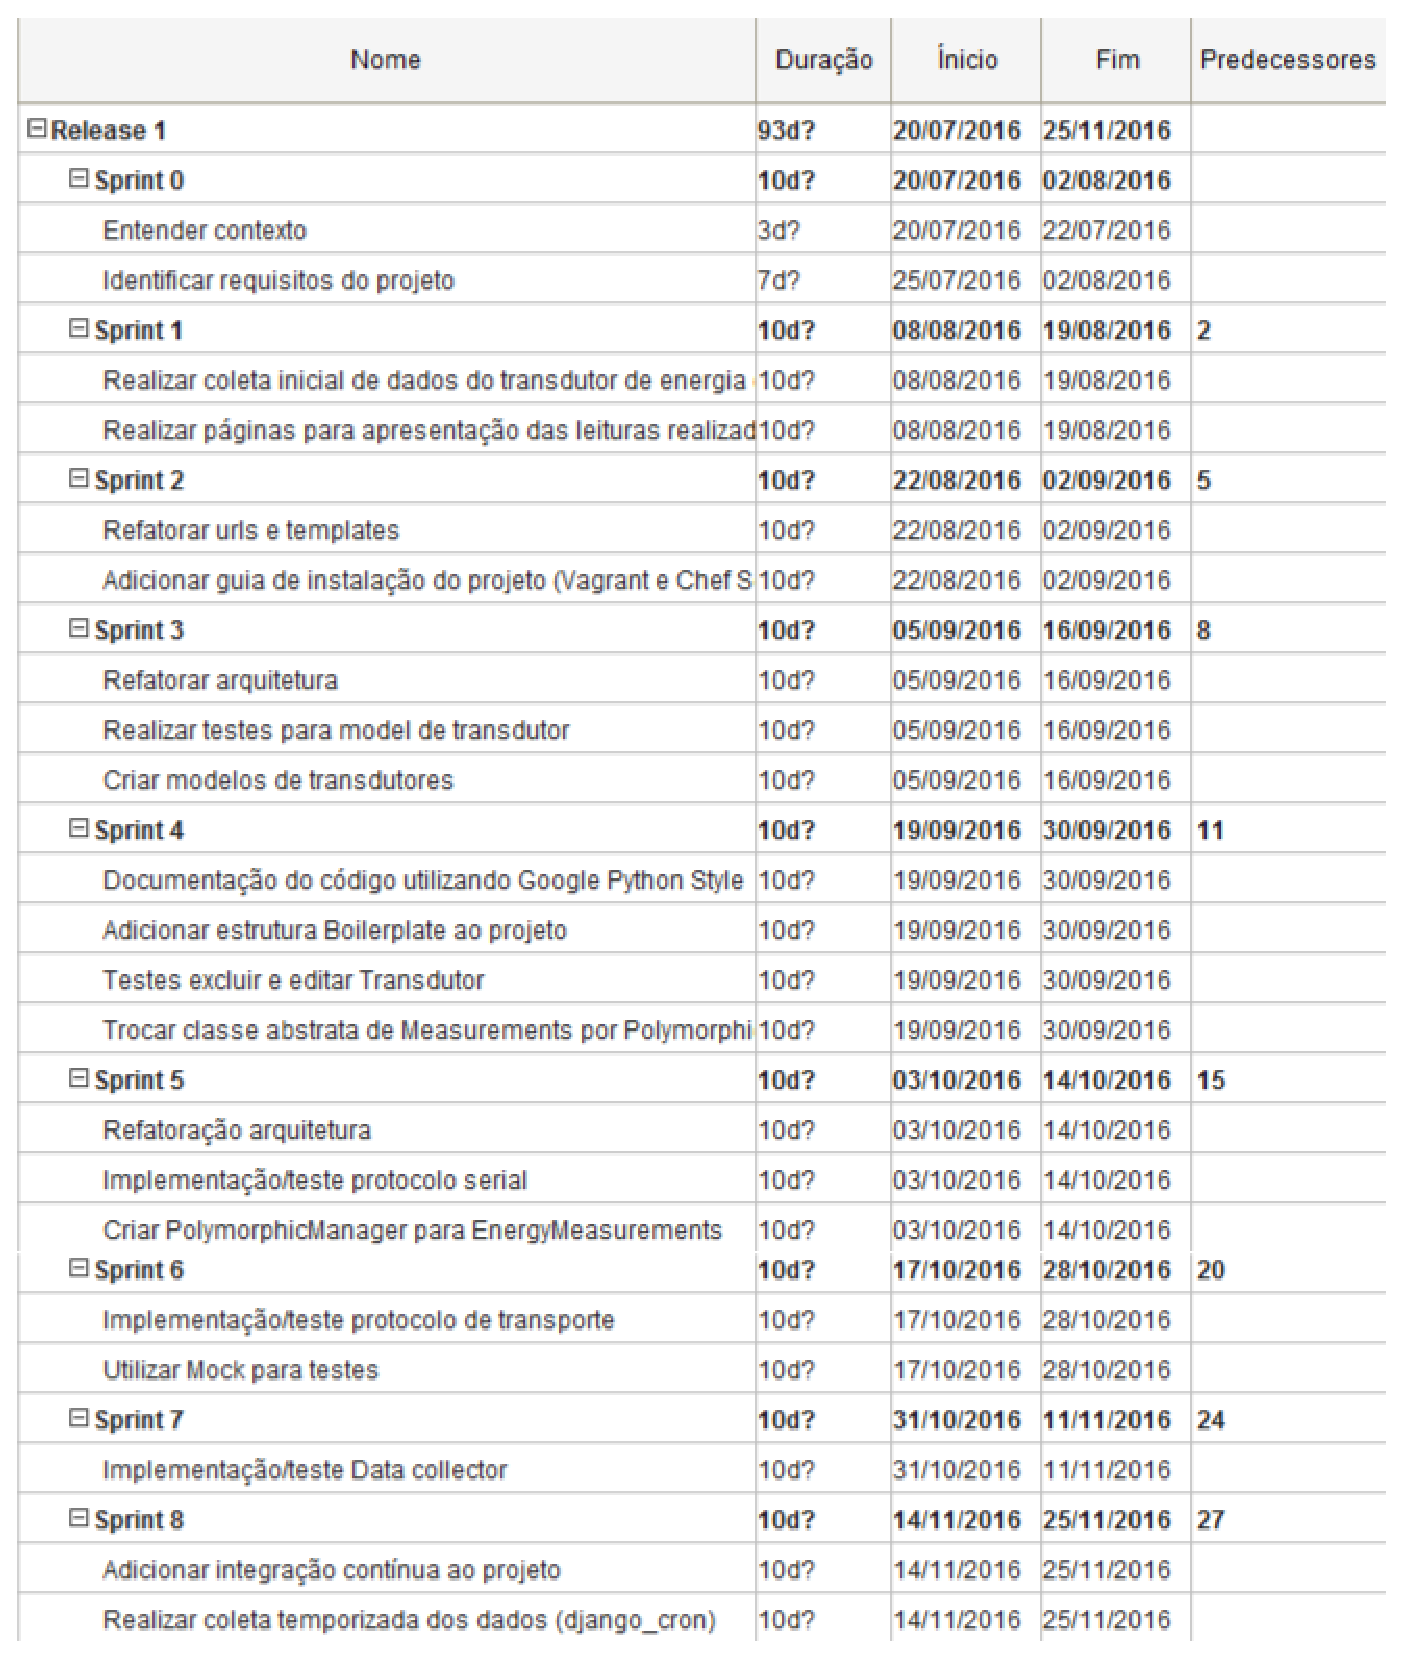
\includegraphics[keepaspectratio=true,scale=0.5]{figuras/cronograma.eps}
    \caption{Cronograma do Projeto. Fonte: autor}
    \label{cronograma}
\end{figure}
% \chapter{Visão Geral do Sistema Desenvolvido}

O levantamento adequado de requisitos de software é crucial para
que possa ser feito um mapeamento das reais necessidades do cliente com
funcionalidades que um sistema deve atender. Sommerville \cite{sommerville_2006}
destingue bem essas abordagens como ``requisitos do usuário'' e ``requisitos do sistema''. Os requisitos de usuários consistem de declarações, em
linguagem natural, que o sistema deve fornecer e restrições que o mesmo deve
operar. Os requisitos de sistema estabelecem de maneira detalhada as
funções e restrições do sistema. Além disso, os requisitos de sistema
classificam-se em funcionais e não funcionais:

\begin{itemize}
    \item Requisitos Funcionais: declaração de funções que o sistema deve fornecer, como o mesmo irá reagir com certas entradas e como deve se comportar para certas situaçoes.
    \item Requisitos Não Funcionais: restrições sobre serviços ou funções oferecidas pelo sistema.
\end{itemize}

Objetivando levantar os requisitos do sistema, realizaram-se reuniões com o
cliente e os requisitos obtidos foram os seguintes:

\begin{itemize}
    \item Funcionais:
    \begin{itemize}
        \item O sistema deve ser capaz de realizar um monitoramento temporal de recursos energéticos.
        \item O sistema deve ser capaz de gerar gráficos com as medições de energia obtidas.
        \item O sistema deve permitir a autenticação de usuários com diferentes níveis de acesso.
        \item O sistema deve permitir o gerenciamento de usuários, prédios e aparelhos de medição.
        \item O sistema deve permitir que usuários atualizem suas informações básicas.
    \end{itemize}
    \item Não Funcionais:
    \begin{itemize}
        \item O
    \end{itemize}
\end{itemize}

Com os requisitos obtidos, realizou-se uma atribuição dos mesmos para
as iterações do projeto, onde cada iteração possuiria um ou mais requisitos,
que eram mapedos, de maneira mais simplificada, em uma \textit{milestone} no repositório oficial do projeto.
As \textit{milestone} representariam um requisito e possuiriam um conjunto
de tarefas (\textit{issues}), que após serem finalizadas, concluiriam
o requisito representado pela mesma.
% \chapter{Gerência de Configuração de \textit{Software}}
Um sistema pode ser definido como a combinação de elementos que entre si interagem e estão organizados para alcançar um ou mais objetivos previamente declarados, onde suas características físicas e funcionais de \textit{hardware} ou \textit{software} representam sua configuração \cite{SWEBOK2014}.

Em uma definição mais formal, a ISO 24765 \cite{iso_24765} define Gerência de Configuração como uma disciplina responsável por: ``identificar e documentar as características funcionais e físicas de um item de configuração, controlar as alterações dessas características, registar e reportar o processamento de alterações e o \textit{status} de implementação, e verificar a conformidade com os requisitos especificados''.

A Gerência de Configuração de \textit{Software} (SCM, do inglês \textit{\textit{Software} Configuration Management}) é um processo que beneficia o gerenciamento de projeto, assim como o seu desenvolvimento, manutenção e atividades referentes à garantia de qualidade \cite{SWEBOK2014}.

O CMMI-DEV \cite{cmmi_dev} define 3 objetivos para a Gerência de Configuração de \textit{Software}:
\begin{itemize}
    \item Estabelecimento de \textit{Baselines}: para cada nova mudança implementada um incremento na evolução do projeto é gerado. Essas mudanças devem possuir um histórico bem definido. As ferramentas de controle de versão facilitam esse trabalho, além de possibilitarem uma programação concorrente. No contexto do projeto utilizou-se a ferramenta Git\footnote{\url{https://git-scm.com/}} como sistema de controle de versão.
    \item Rastreamento e Controle de Mudanças: durante o desenvolvimento de \textit{software} mudanças ocorrem com frequência. É necessário portanto que as mesmas sejam armazenadas, analisadas e agrupadas de acordo com o histórico e suas prioridades. Utilizou-se o \textit{software} livre GitLab CE\footnote{\url{https://gitlab.com/gitlab-org/gitlab-ce}} para realizar toda a hospedagem do projeto\footnote{\url{https://gitlab.com/brenddongontijo/SME-UnB}} e o controle de mudanças.
    \item Estabelecimento de Integridade: verificar se a construção de um sistema, atendendo suas configurações pré-estabelecidas, é bem sucedida a cada nova mudança registrada.
\end{itemize}
% \chapter{Evolução do Sistema}

\section{Sprint 01 (25/07/2016 à 05/08/2016) - Coleta Inicial de Dados do Transdutor}
Buscando realizar uma primeira análise do transdutor instalado na Universidade, verificando se a comunicação com o mesmo poderia ser realizada de maneira efetiva, realizou-se o módulo \textit{data\_reader} contendo as seguintes classes:
\begin{itemize}
    \item Transductor: representação de um transdutor.
    \item Measurements: representação das medições de energia realizadas pelo transdutor.
    \item CommunicationProtocol: acoplamento dos protocolos de transporte e serial, visando realizar uma comunicação com o transdutor.
\end{itemize}

A figura \ref{sprint01arq} representa a arquitetura inicial do projeto, onde basicamente um transdutor possui várias medições de energia e, dependendo do seu modelo, pode utilizar diferentes protocolos de comunicação.

\begin{figure}[!htpb]
    \centering
    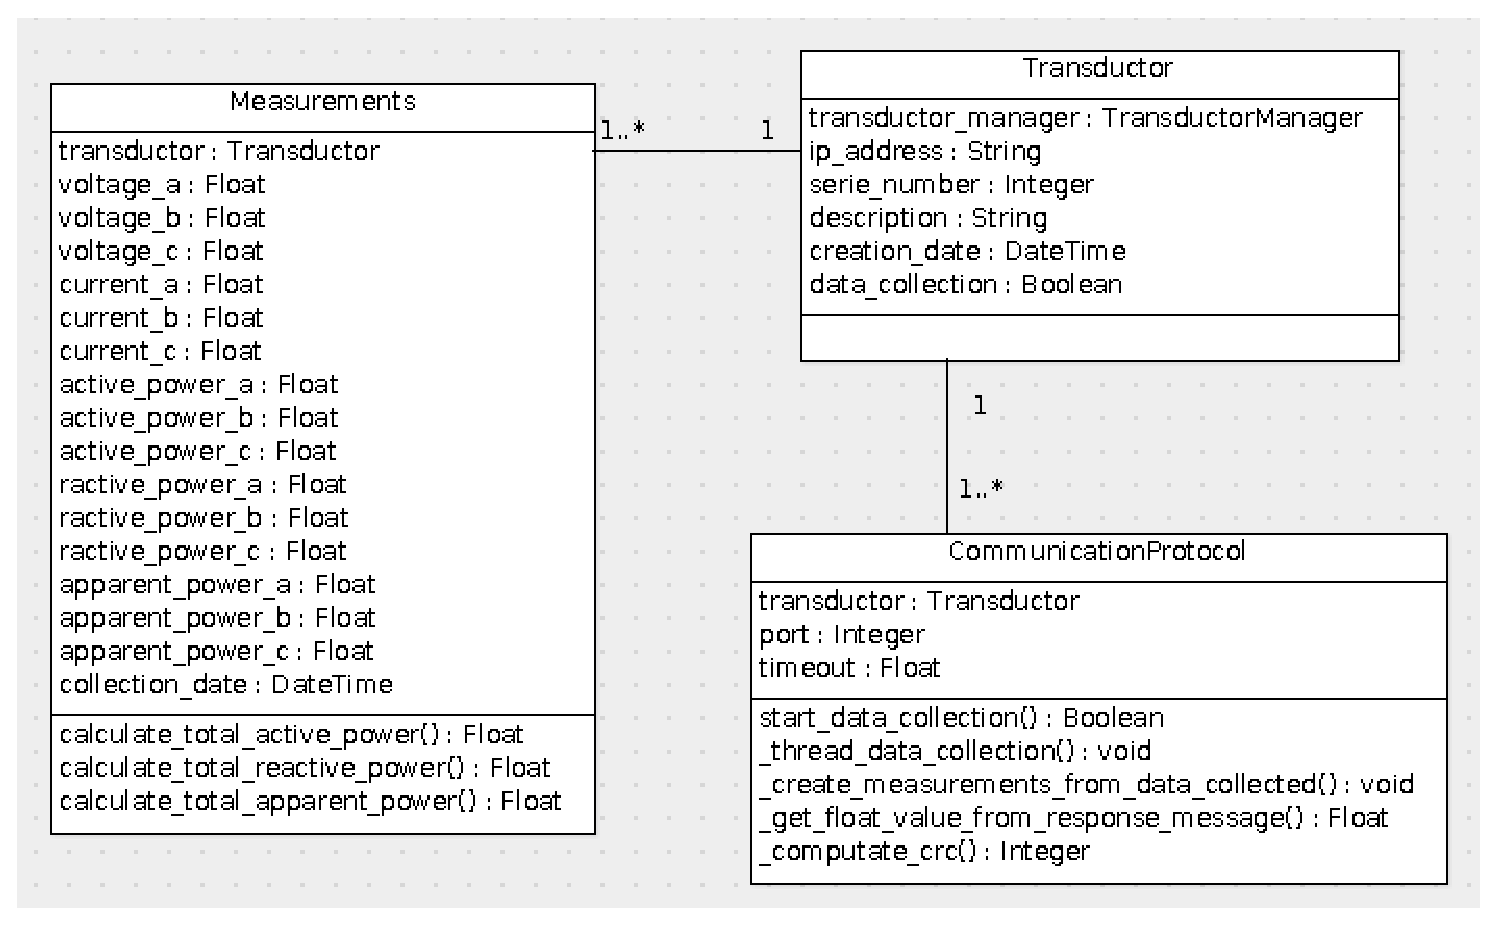
\includegraphics[keepaspectratio=true,scale=0.6]{figuras/sprint01arq.eps}
    \caption{Arquitetura SME-UnB \textit{Sprint 01}. }
    \label{sprint01arq}
\end{figure}

\vfill
\pagebreak

Foram realizadas algumas telas, figuras \ref{dados02} e \ref{dados01}, contendo os dados de energia coletados para apresentação ao usuário.

\begin{figure}[!htpb]
    \centering
    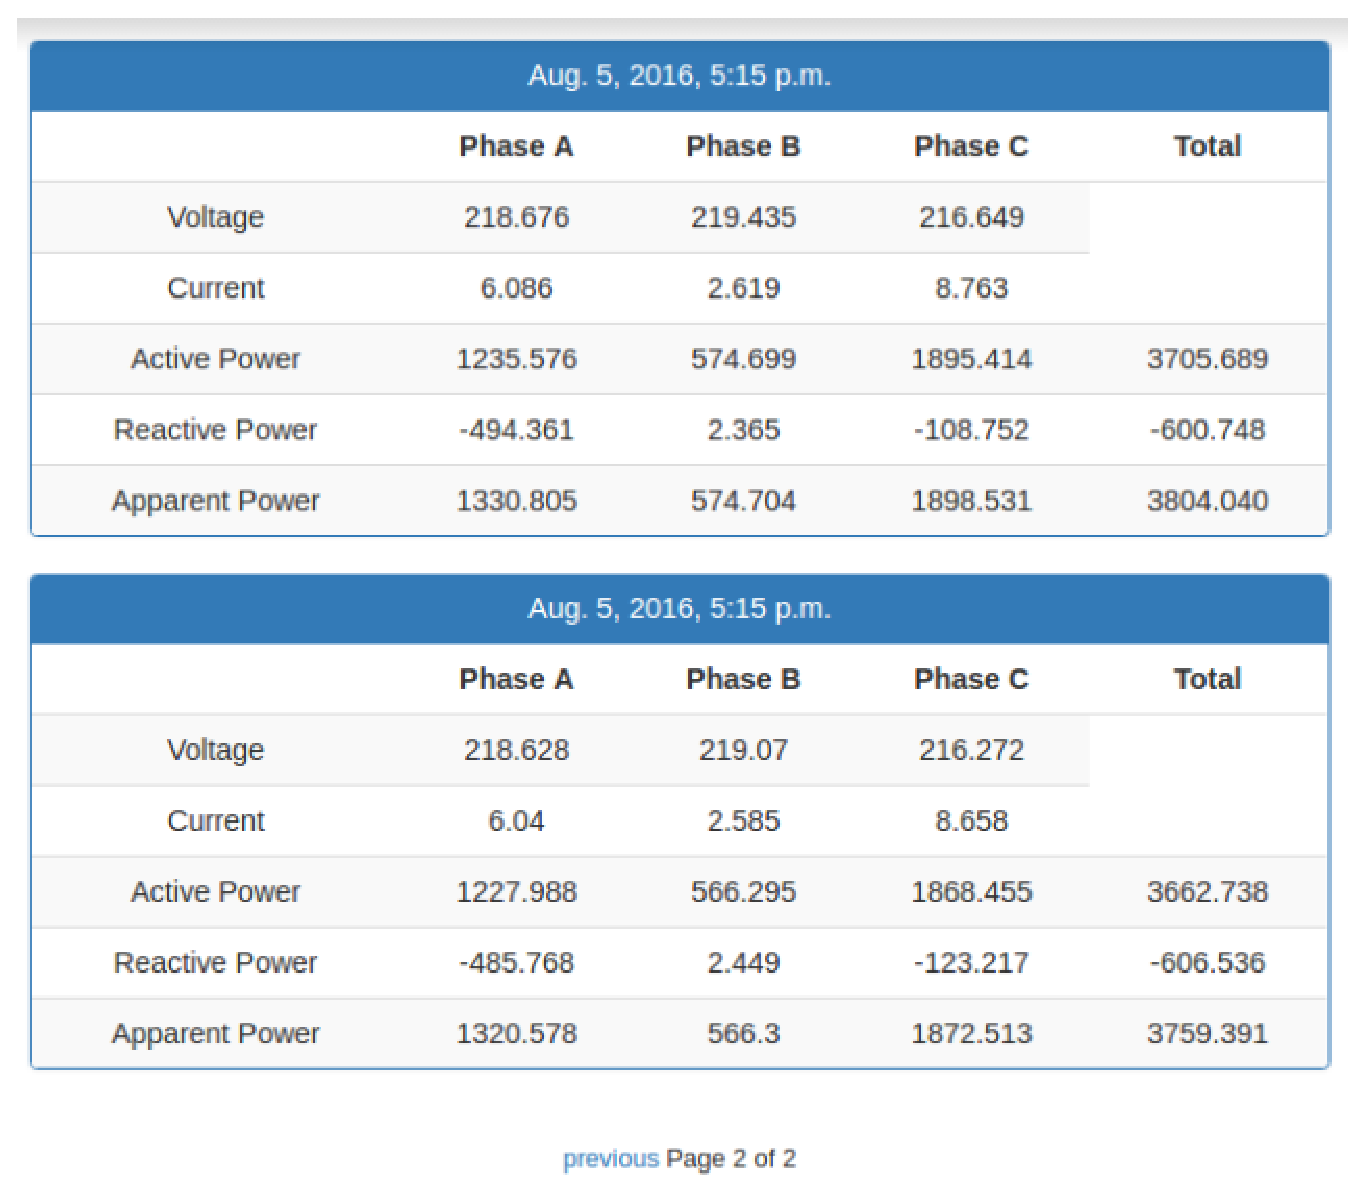
\includegraphics[keepaspectratio=true,scale=0.5]{figuras/coleta_dados_02.eps}
    \caption{Página de apresentação dos transdutores.}
    \label{dados02}
\end{figure}

\begin{figure}[!htpb]
    \centering
    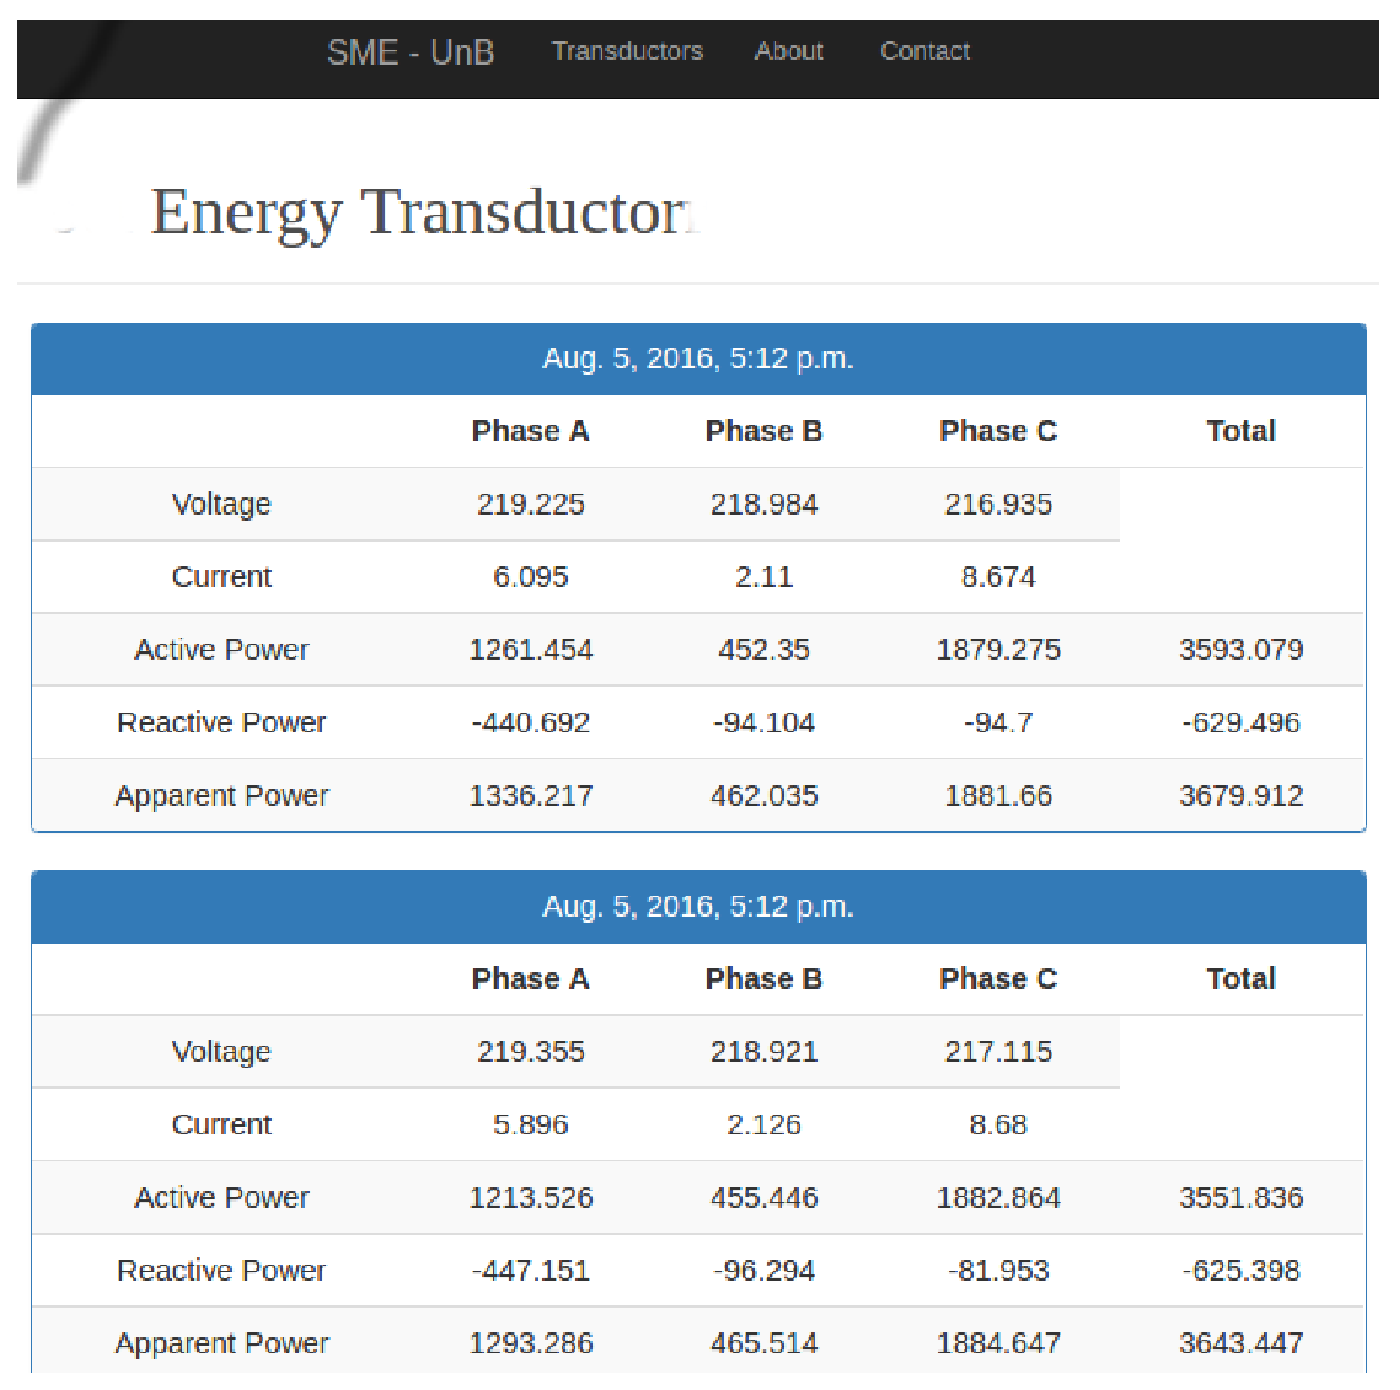
\includegraphics[keepaspectratio=true,scale=0.5]{figuras/coleta_dados_01.eps}
    \caption{Página apresentação medições de energia.}
    \label{dados01}
\end{figure}

\vfill
\pagebreak

\section{Sprint 02 (08/08/2016 à 19/08/2016) - Refatorações de \textit{Urls}/\textit{Templates} e Guia de Instalação}
Após analisadas as \textit{urls} e \textit{templates} do projeto verificou-se que havia muitas rotas desnecessárias e não havia um padrão para os templates, o que estava gerando confusão na hora de criar novas páginas para a aplicação. Tendo em mente tais problemas essa sprint buscou realizar uma refatoração dos mesmos.

Realizou-se um guia de instalação\footnote{\url{https://gitlab.com/brenddongontijo/SME-UnB/wikis/instalation-guide/}} para o ambiente de desenvolvimento utilizando as ferramentas \textit{Vagrant}\footnote{\url{https://www.vagrantup.com/}} e \textit{Chef Solo}\footnote{\url{https://docs.chef.io/chef_solo.html}}, visando auxiliar novos desenvolvedores a contribuirem com o projeto.

\section{Sprint 03 (22/08/2016 à 02/09/2016) - Reestruturação Arquitetura e Primeiros Testes}
Realizou-se uma reunião com o orientador visando reestruturar a arquitetura. Primordialmente, tendo em vista que os tradutores podem possuir diferentes tipos de medições, foram definidas duas classes abstratas: Transductor e Measurements. A partir dessas classes surgiram as especializações de transdutores de energia (EnergyTransductor) e medições de energia (EnergyMeasurements). Além disso, percebeu-se a necessidade de criação de um modelo de transdutor (TransductorModel), o qual possuiria informações específicas do mesmo, como endereço dos registradores importantes, protocolo serial e de transporte utilizados. A figura \ref{sprint03arq} ilustra a evolução da arquitetura realizada nessa sprint.

\begin{figure}[!htpb]
    \centering
    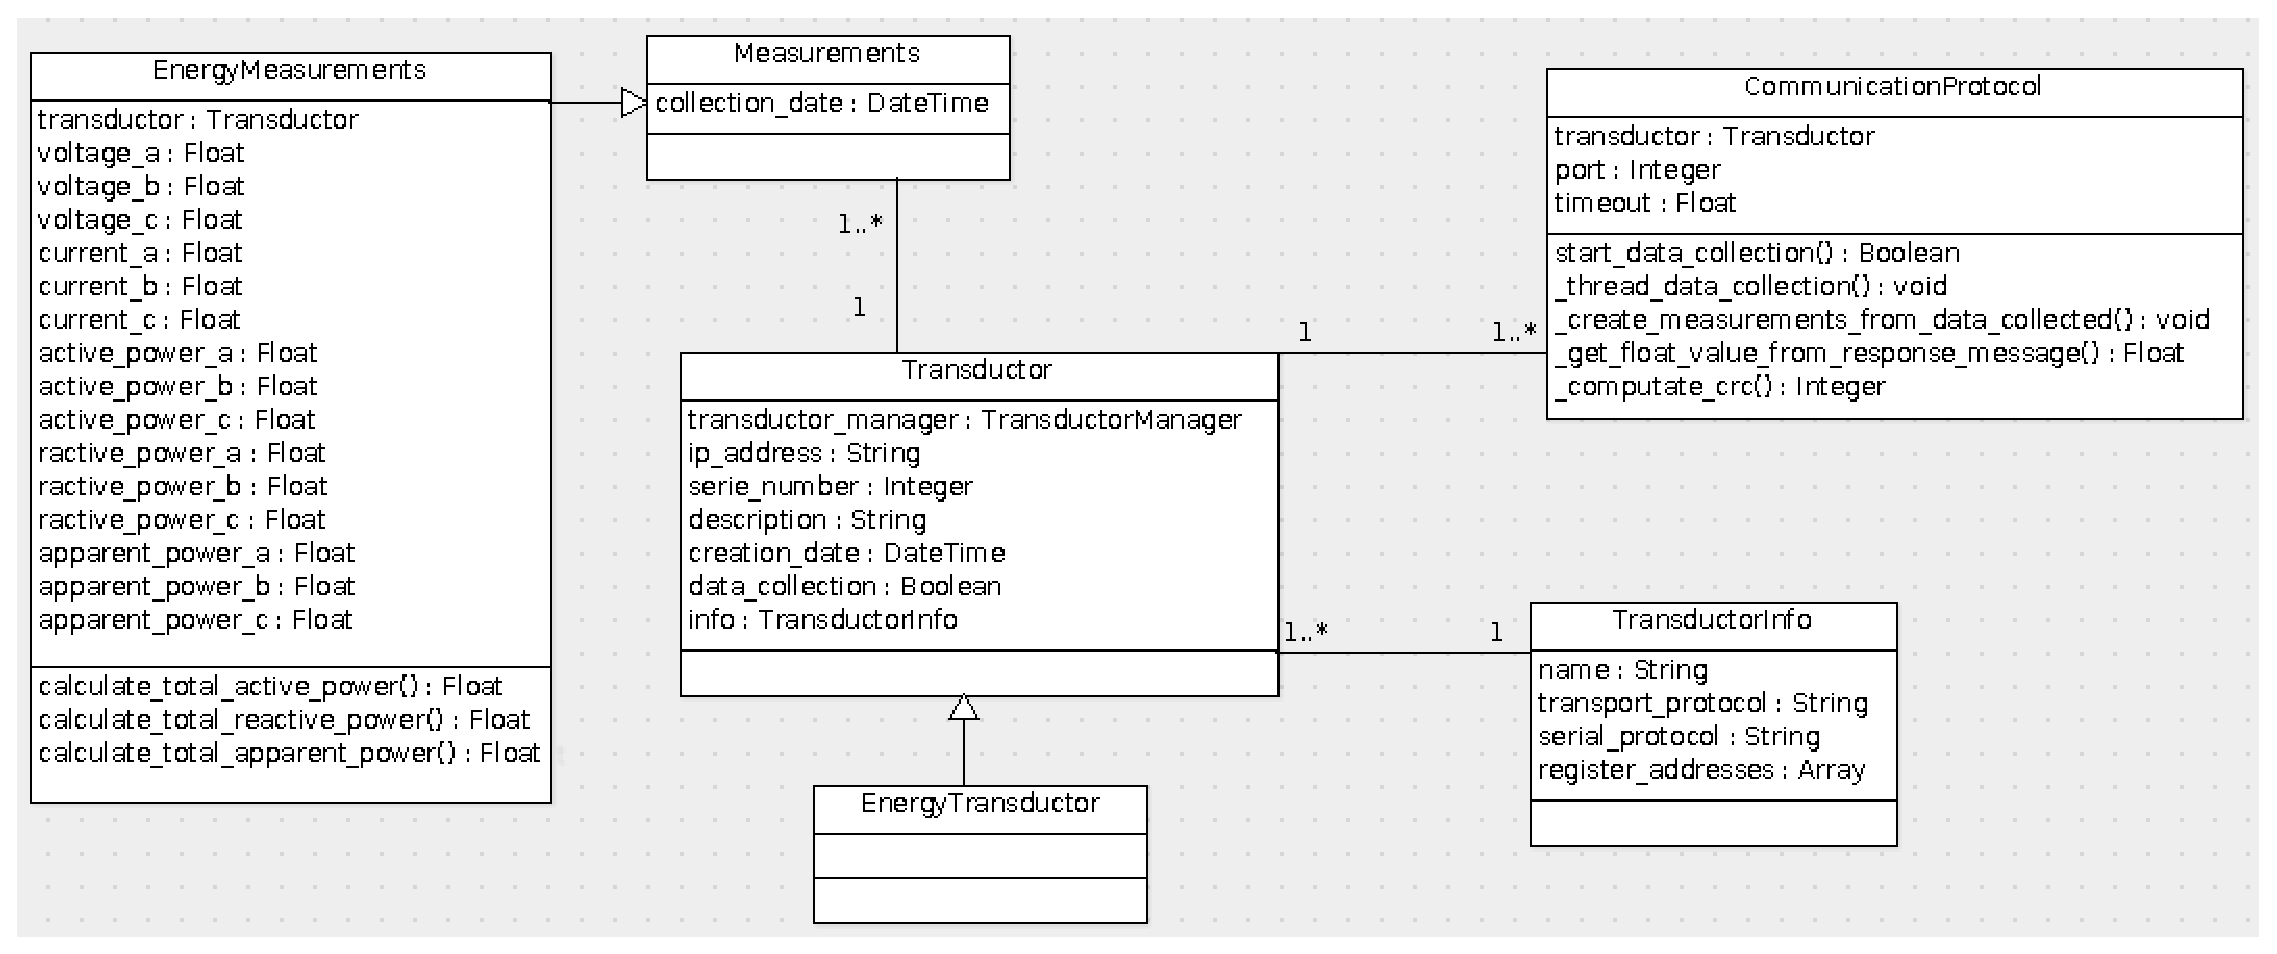
\includegraphics[scale=0.6,angle=90]{figuras/sprint03arq.eps}
    \caption{Arquitetura SME-UnB Sprint 03. }
    \label{sprint03arq}
\end{figure}

\vfill
\pagebreak

Nessa sprint foi realizado um primeiro contato com os testes e ao seu fim obtivo-se uma cobertura de 71\%, conforme a figura \ref{cobertura01}.

\begin{figure}[!htpb]
    \centering
    \includegraphics[keepaspectratio=true,scale=0.5]{figuras/cobertura01.eps}
    \caption{Cobertura Total de Código Sprint 03. }
    \label{cobertura01}
\end{figure}

\section{Sprint 04 (05/09/2016 à 16/09/2016) - Documentação de Código e Estrutura \textit{Boilerplate}}
Buscando deixar o código mais compreensível, realizou-se uma documentação das principais classes do sistema utilizando os padrões de \textit{docstrings}\footnote{\url{https://www.python.org/dev/peps/pep-0257/}} definidos pelo \textit{Google Python Style}\footnote{\url{http://google.github.io/styleguide/pyguide.html}}. A figura \ref{documentacao01} ilustra um exemplo realizado no projeto.

\begin{figure}[!htpb]
    \centering
    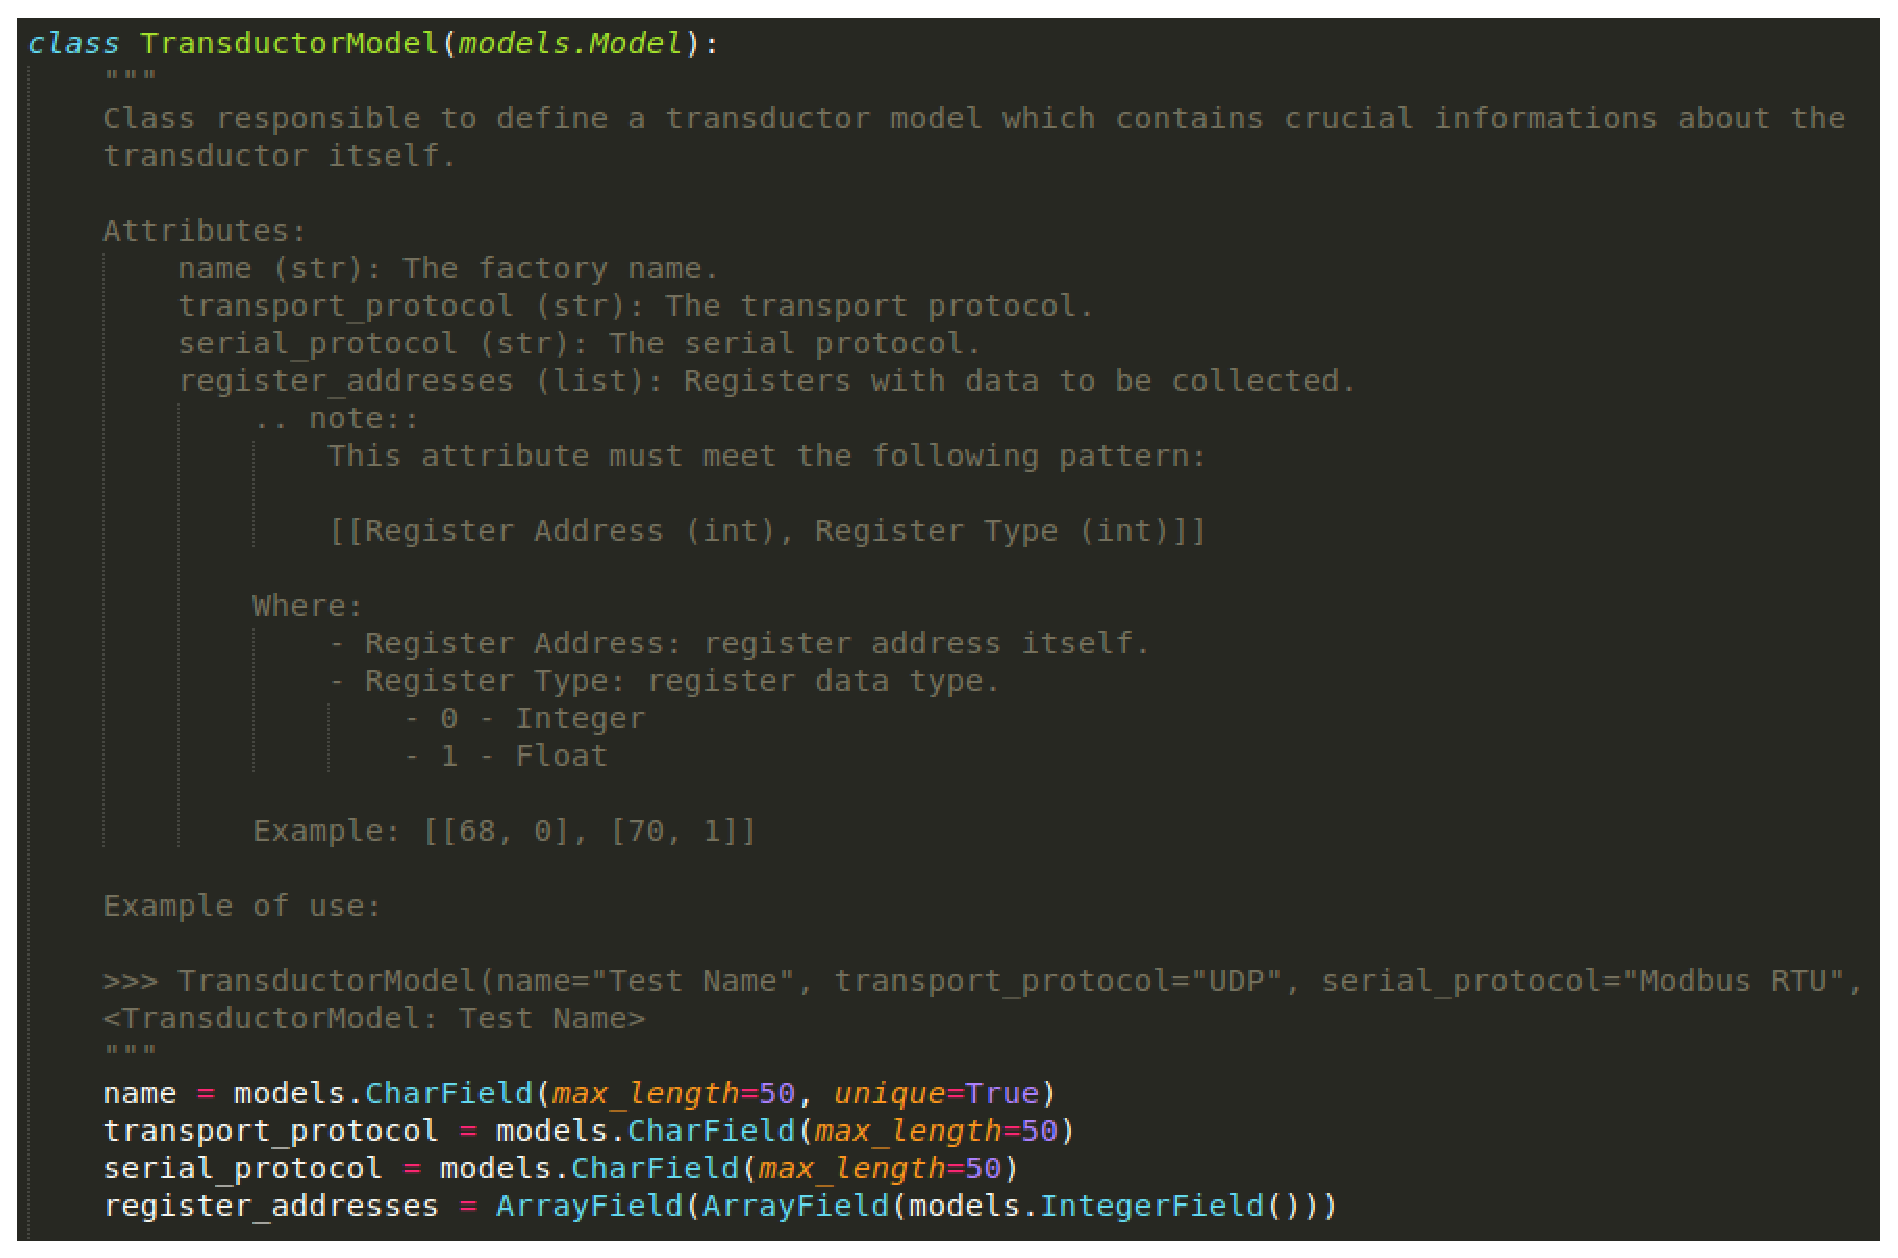
\includegraphics[keepaspectratio=true,scale=0.5]{figuras/documentacao01.eps}
    \caption{Exemplo de Documentação Utilizando \textit{Google Python Style}. }
    \label{documentacao01}
\end{figure}

A estrutura \textit{Boilerplate}\footnote{\url{https://github.com/fabiommendes/python-boilerplate}} foi adicionada ao projeto com o objetivo de realizar uma melhor estruturação dos módulos e realizar pré-configurações para ambientes de desenvolvimendo/produção, assim como no auxílio para utilização das ferramentas \textit{Sphinx} e \textit{Coverage}.

\section{Sprint 05 (19/09/2016 à 30/09/2016) - Refatoração Arquitetural e Protocolo Serial}
Tendo em vista o acúmulo de responsabilidades dentro da classe CommunicationProtocol, realizou-se uma fatoração buscando separá-la em duas classes abstratas: TransportProtocol e SerialProtocol. A partir dessas classes definiram-se as especializações referentes ao protocolo UDP (UdpProtol) e \textit{Modbus} em modo RTU (ModbusRTU), os quais são utilizados especificamente pelo modelo de transdutor instalado na Universidade. Além dessas mudanças criou-se uma nova classe chamada EnergyOperations, responsável por realizar cálculos matemáticos com os dados de energia coletados.

Além das mudanças arquiteturais, foram implementadas e testadas as classes SerialProtocol, ModbusRTU e EnergyOperations. Obteve-se uma cobertura de 96\% ao fim da sprint.

\section{Sprint 06 (03/10/2016 à 14/10/2016) - Protocolo de Transporte e Testes com \textit{Mock}}
Após implementado o protocolo serial, realizou-se o desenvolvimento do protocolo de transporte. Sua principal função é comunicar-se com o transdutor e tratar as questões referentes a \textit{timeouts} e tentativas consecutivas de envio de requisições. Além disso, foram refatorados os testes do sistema utilizando \textit{Mocks}\footnote{\url{https://docs.python.org/3/library/unittest.mock.html}}, objetivando maior desempenho e unitariedade dos métodos. A figura \ref{exemplo_mock} ilustra um exemplo de teste da classe UdpProtocol utilizando \textit{Mock}.

\begin{figure}[!htpb]
    \centering
    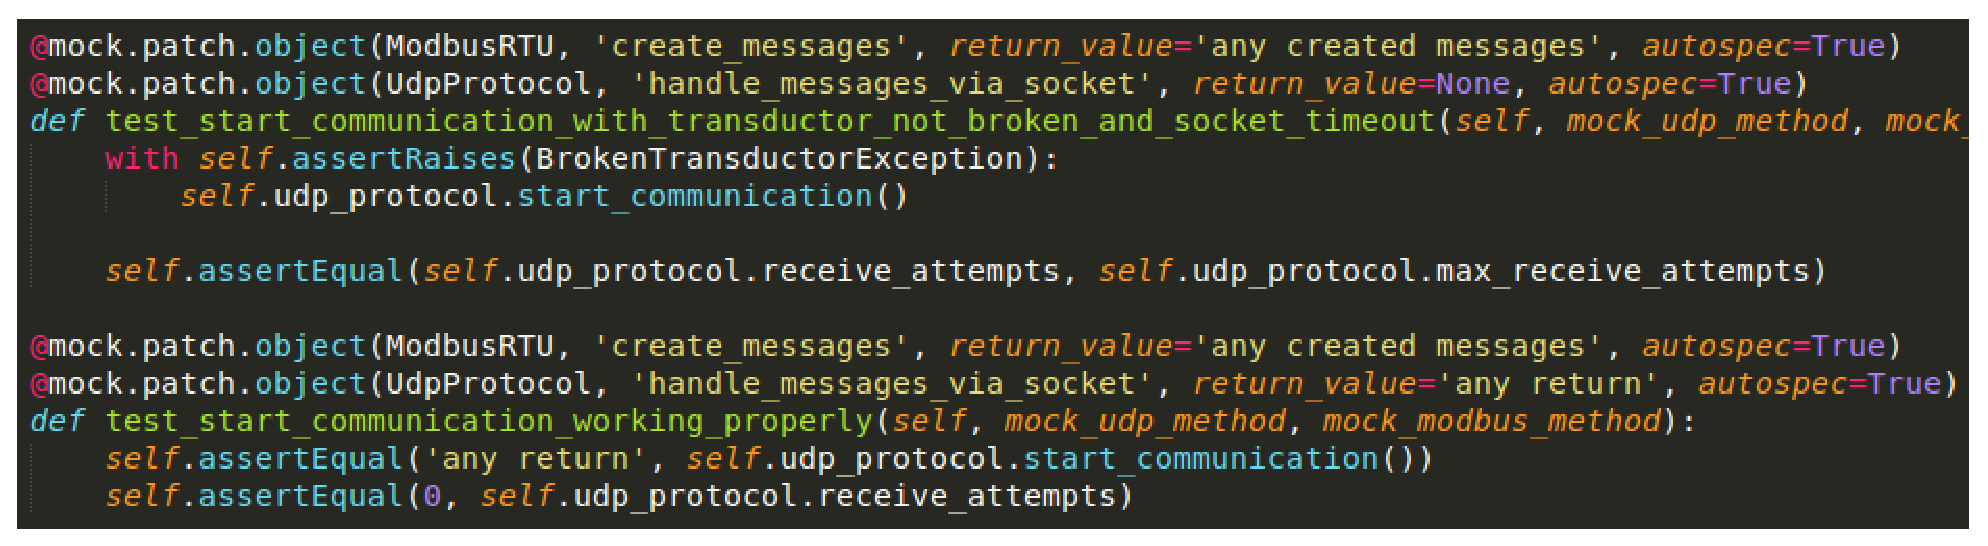
\includegraphics[keepaspectratio=true,scale=0.5]{figuras/exemplo_mock.eps}
    \caption{Exemplo de Teste utilizando \textit{Mock}. }
    \label{exemplo_mock}
\end{figure}

\section{Sprint 07 (17/10/2016 à 28/10/2016) - Gerenciador para Coleta de Dados}
Após implementar os protocolos de transporte e serial verificou-se a necessidade de uma classe que realizasse toda a comunicação dos mesmos, ou seja, desempenhasse a coleta das medições de cada transdutor. Essa classe foi definida como DataCollector e utiliza os princípios de \textit{threads}\footnote{\url{https://docs.python.org/2/library/threading.html}} para inicar simultaneamente a coleta de dados de todos os transdutores.

A cobertura total de código obtida ao fim da sprint foi de 95\%.

\section{Sprint 08 - \textit{Cron Job} e Integração Contínua}
Objetivando executar a coleta de dados de maneira temporizada, realizou-se a classe DataCollectCronJob, a qual foi programada para ser executada a cada 1 minuto. Além disso, configurou-se o serviço de integração contínua do \textit{Gitlab CI}, figura \ref{gitlabci}, que basicamente cria um ambiente do zero, instala as dependências do projeto, realiza a suíte de testes e verifica se o código está devidamente de acordo com as normas da PEP 8.
\begin{figure}[!htpb]
    \centering
    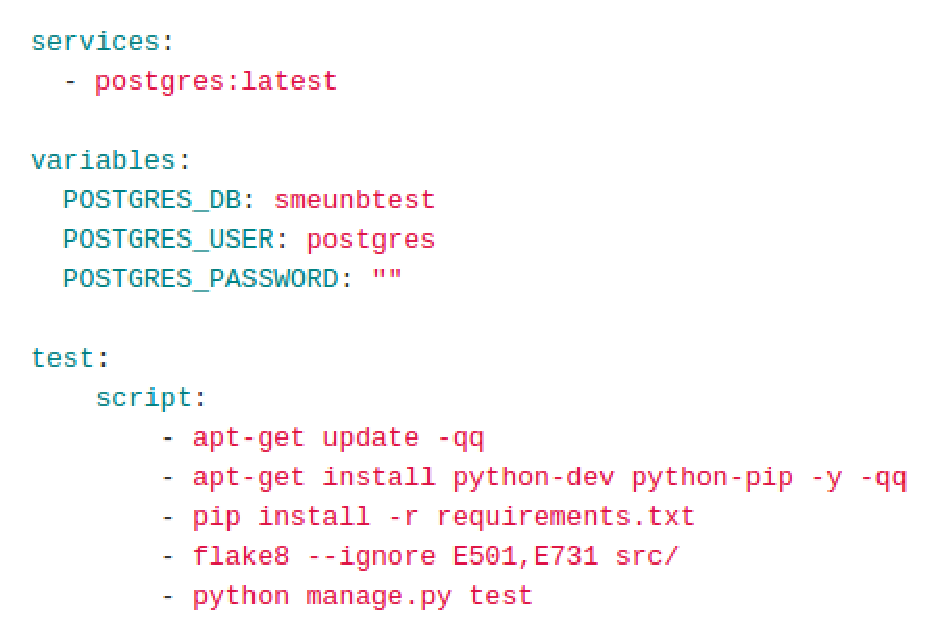
\includegraphics[keepaspectratio=true,scale=0.6]{figuras/gitlabci.eps}
    \caption{\textit{Script} de Integração Contínua. }
    \label{gitlabci}
\end{figure}

\begin{figure}[!htpb]
    \centering
    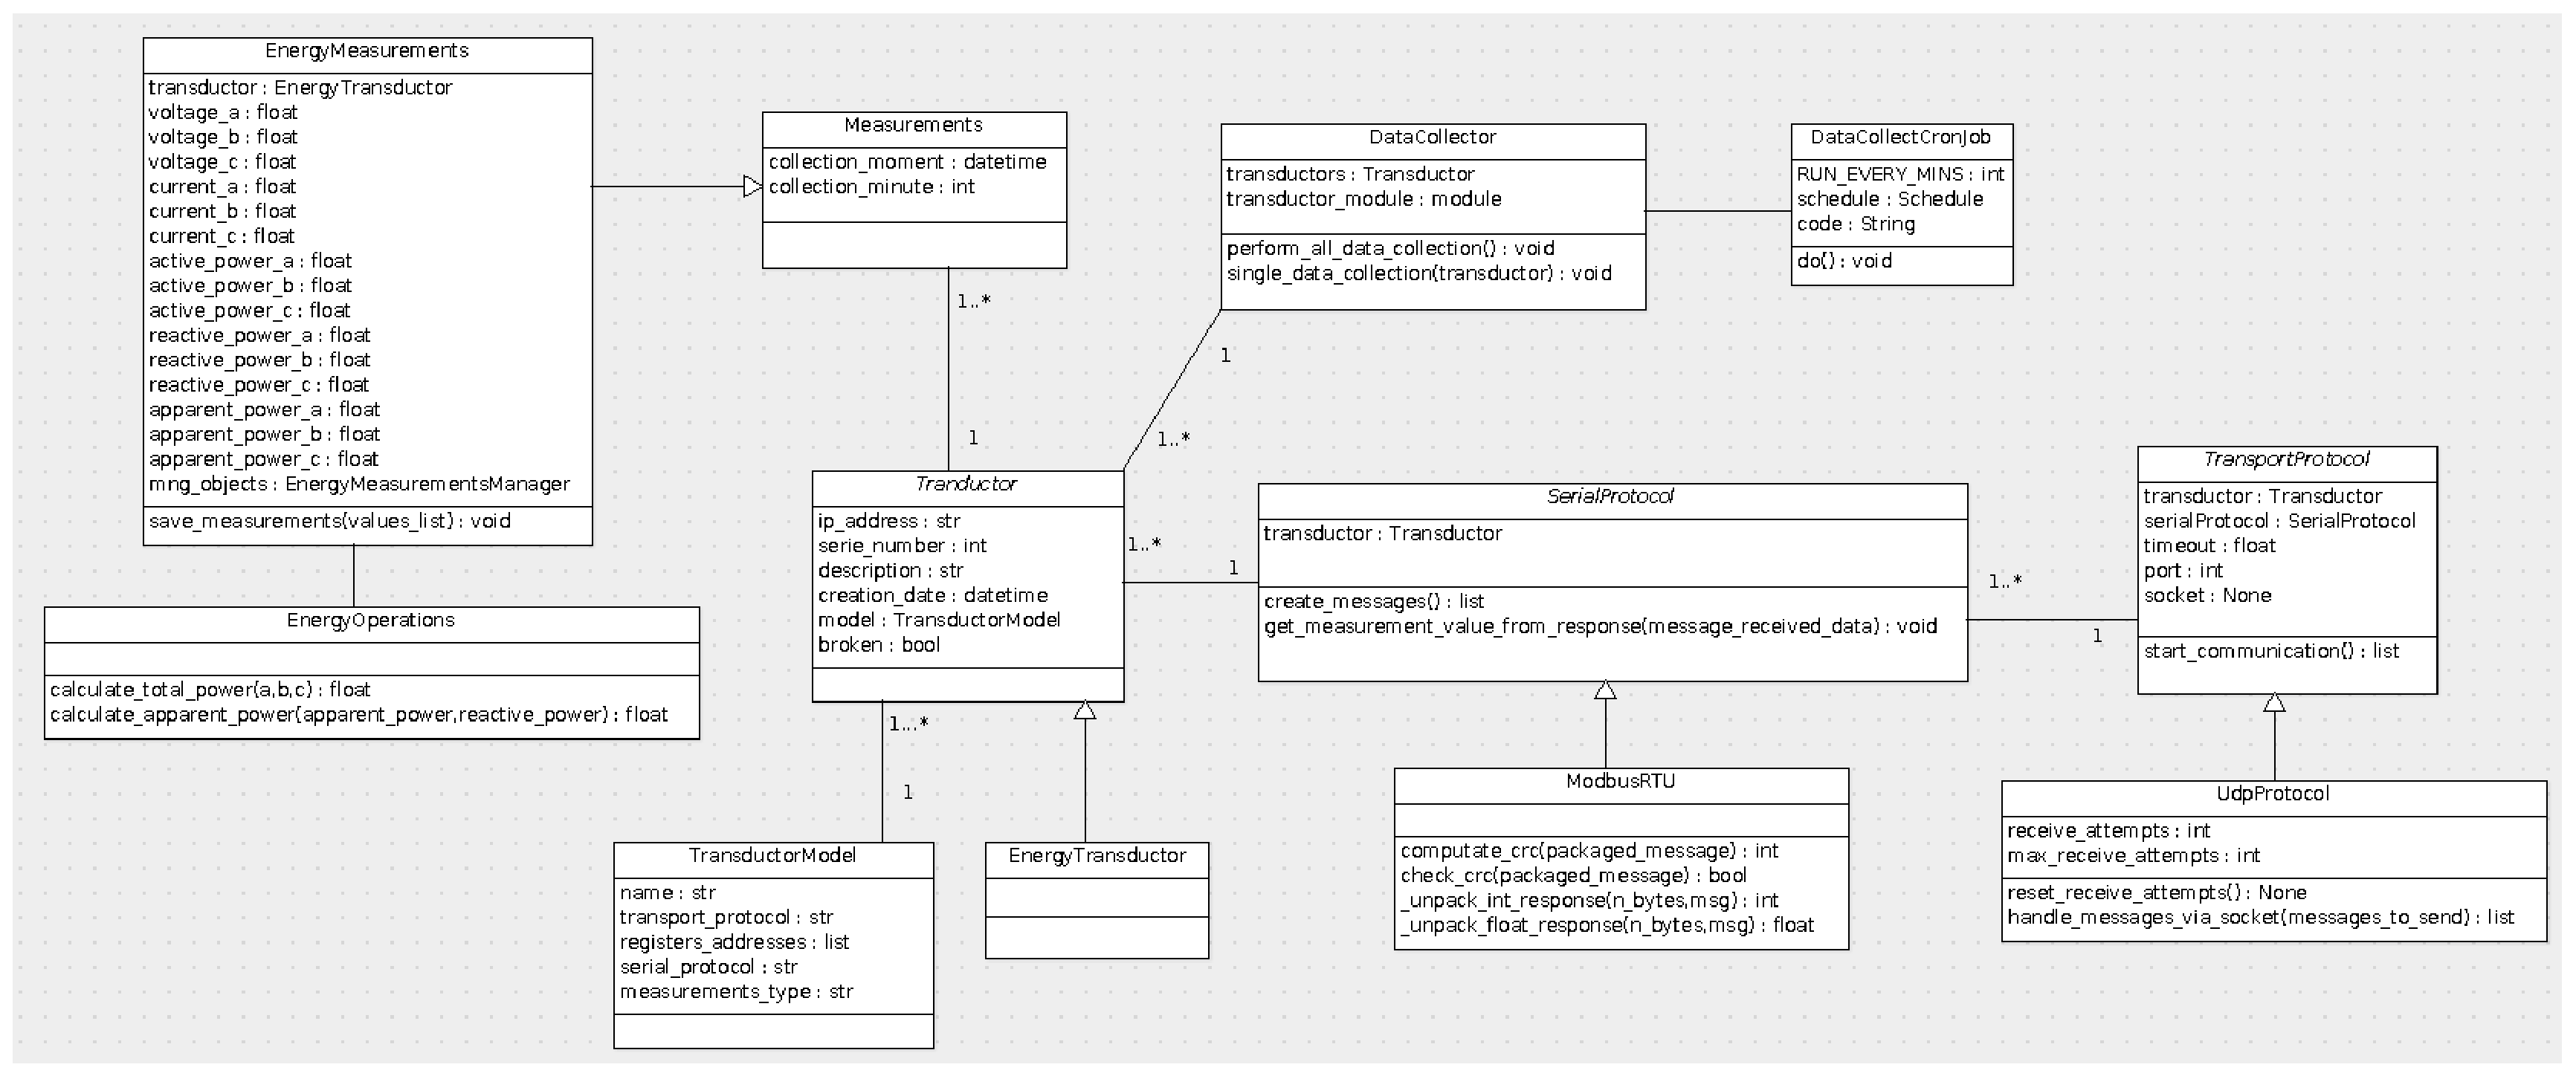
\includegraphics[scale=0.4,angle=90]{figuras/sprint08arq.eps}
    \caption{Arquitetura Final SME-UnB. }
    \label{sprint08arq}
\end{figure}

\begin{figure}[!htpb]
    \centering
    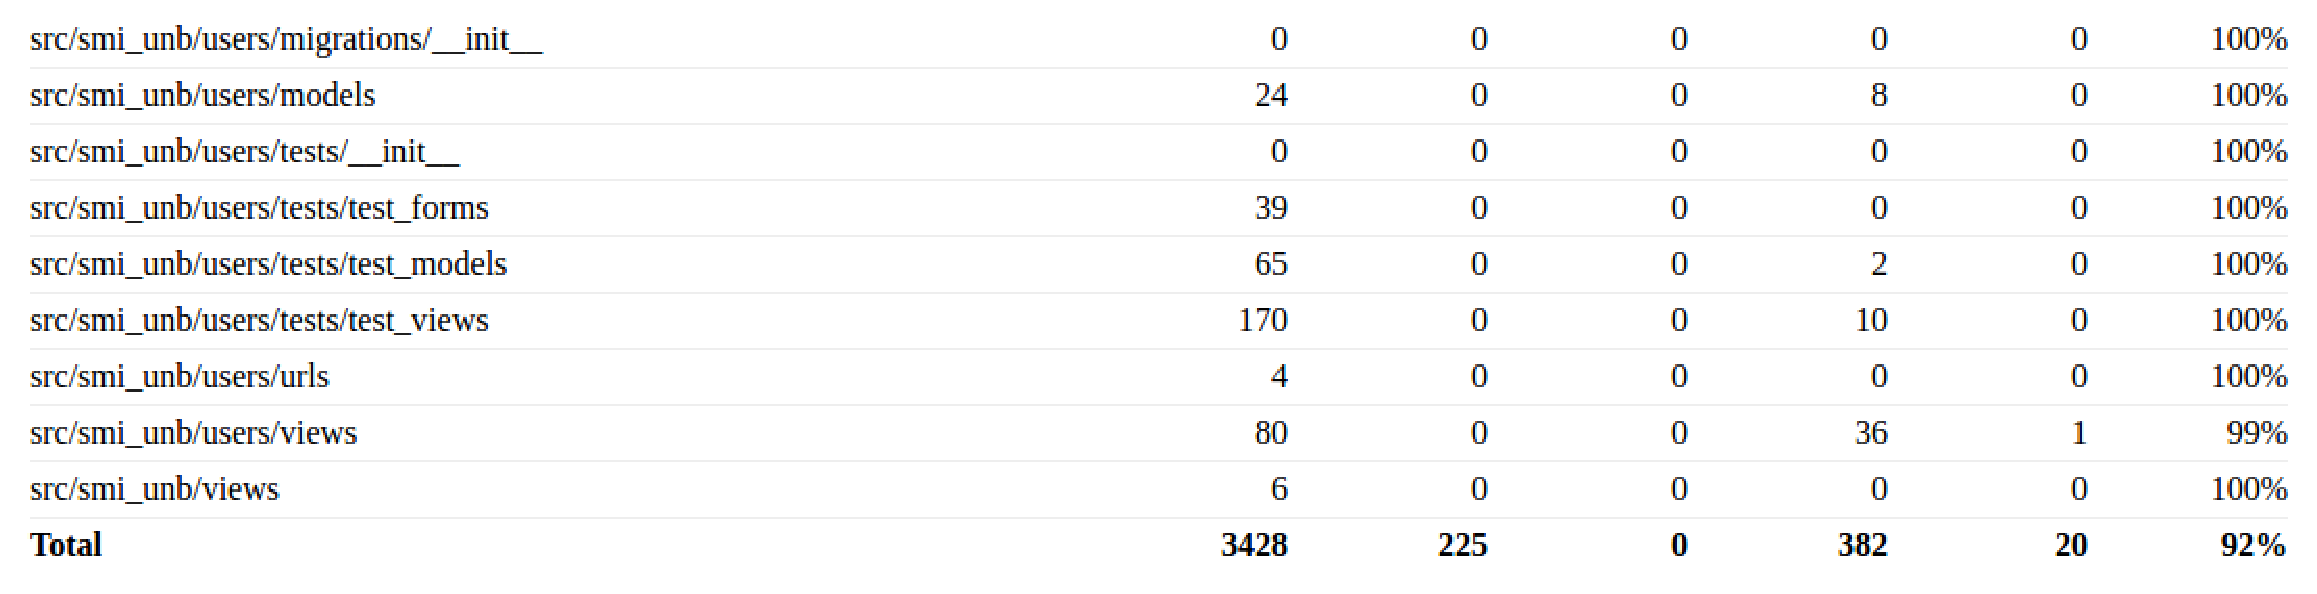
\includegraphics[keepaspectratio=true,scale=0.5]{figuras/cobertura05.eps}
    \caption{Cobertura Final de Código Obtida. }
    \label{cobertura05}
\end{figure}

\bookmarksetup{startatroot}

\postextual

\bibliography{bibliografia}
%\begin{apendicesenv}

\partapendices

\chapter{Integração Contínua}
\begin{python}[caption={\textit{Log} de integração contínua do SMI-UnB}, captionpos=b, label={integracao_cont}]
Running with gitlab-ci-multi-runner 9.3.0-rc.2 (110d530)
  on docker-auto-scale (e11ae361)
Using Docker executor with image python:3.5 ...
Starting service postgres:latest ...
Pulling docker image postgres:latest ...
Using docker image postgres:latest for postgres service...
Waiting for services to be up and running...
Using docker image sha256 for predefined container...
Pulling docker image python:3.5 ...
Using docker image python:3.5 for build container...
Running on runner-e11ae361-project-1216906...
Cloning repository...
Cloning into '/builds/brenddongontijo/SMI-UnB'...
Checking out e70a256f as master...
Skipping Git submodules setup
$ apt-get update -qq
$ apt-get install python3-pip -y -qq
# Installing packages...
$ flake8 src/ --exclude migrations
$ coverage run manage.py test \
smi_unb --settings=smi_unb.settings_runner
# Running tests...
----------------------------------------------
Ran 192 tests in 17.081s
OK
Creating a new SECRET_KEY at security/secret_key.dat
Running server in DEBUG mode. Plese do *not* go to production!
Documentation files not found: disabling tests!
Creating test database for alias 'default'...
Destroying test database for alias 'default'...
$ coverage report
# Coverage report...
Job succeeded
\end{python}

\chapter{Cobertura Total de Código}
\begin{figure}[!htpb]
    \centering
    \includegraphics[keepaspectratio=true,scale=0.45]{figuras/cobertura01.eps}
    \caption{Primeira parte da cobertura do SMI-UnB.}
    \label{cobertura01}
\end{figure}

\begin{figure}[!htpb]
    \centering
    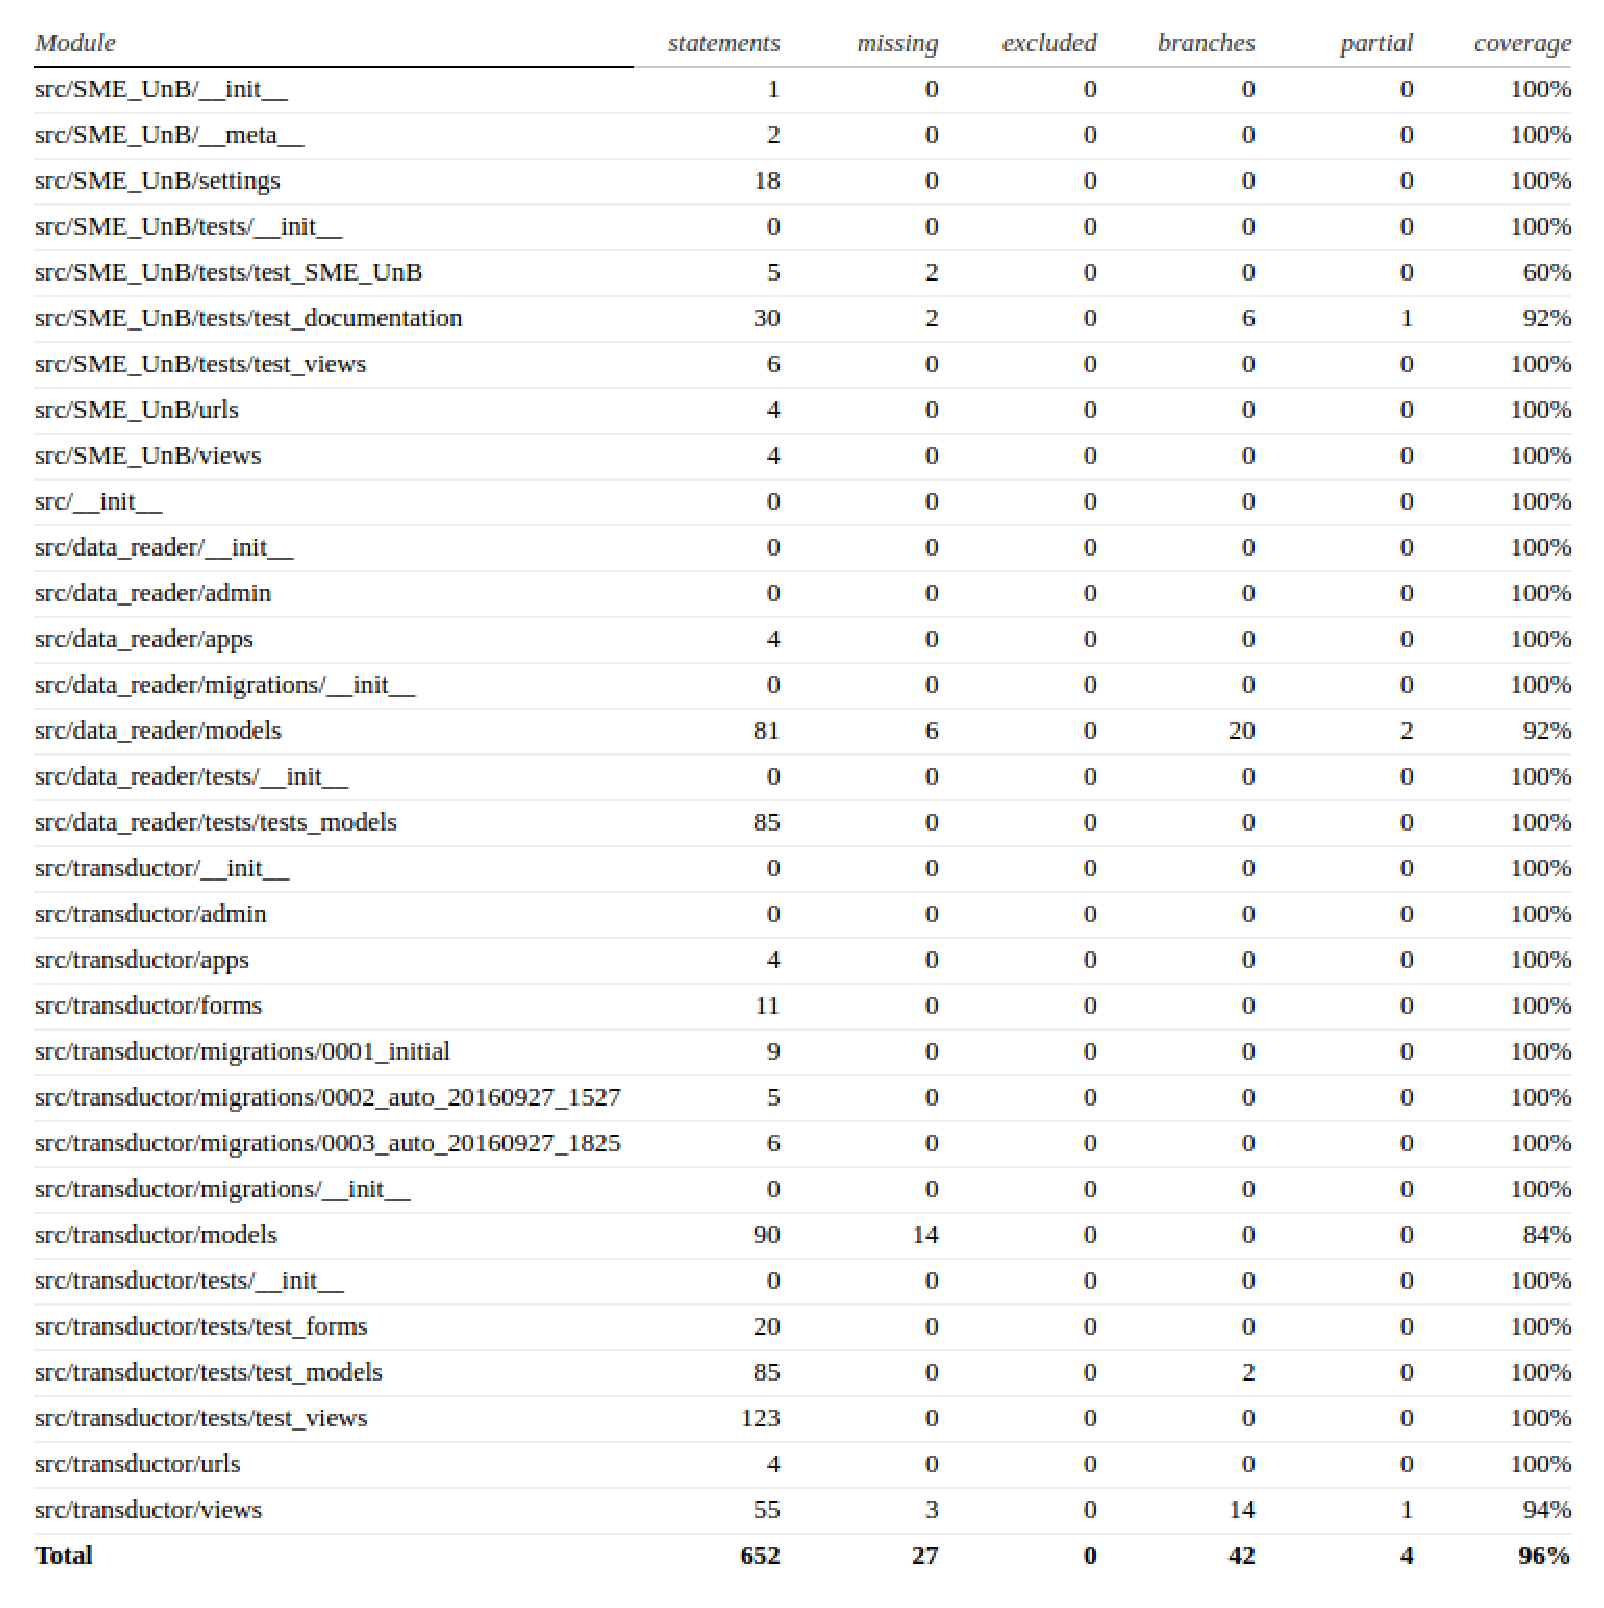
\includegraphics[keepaspectratio=true,scale=0.45]{figuras/cobertura02.eps}
    \caption{Segunda parte da cobertura do SMI-UnB.}
    \label{cobertura02}
\end{figure}

\chapter{Imagens da Aplicação}
\begin{figure}[!htpb]
    \centering
    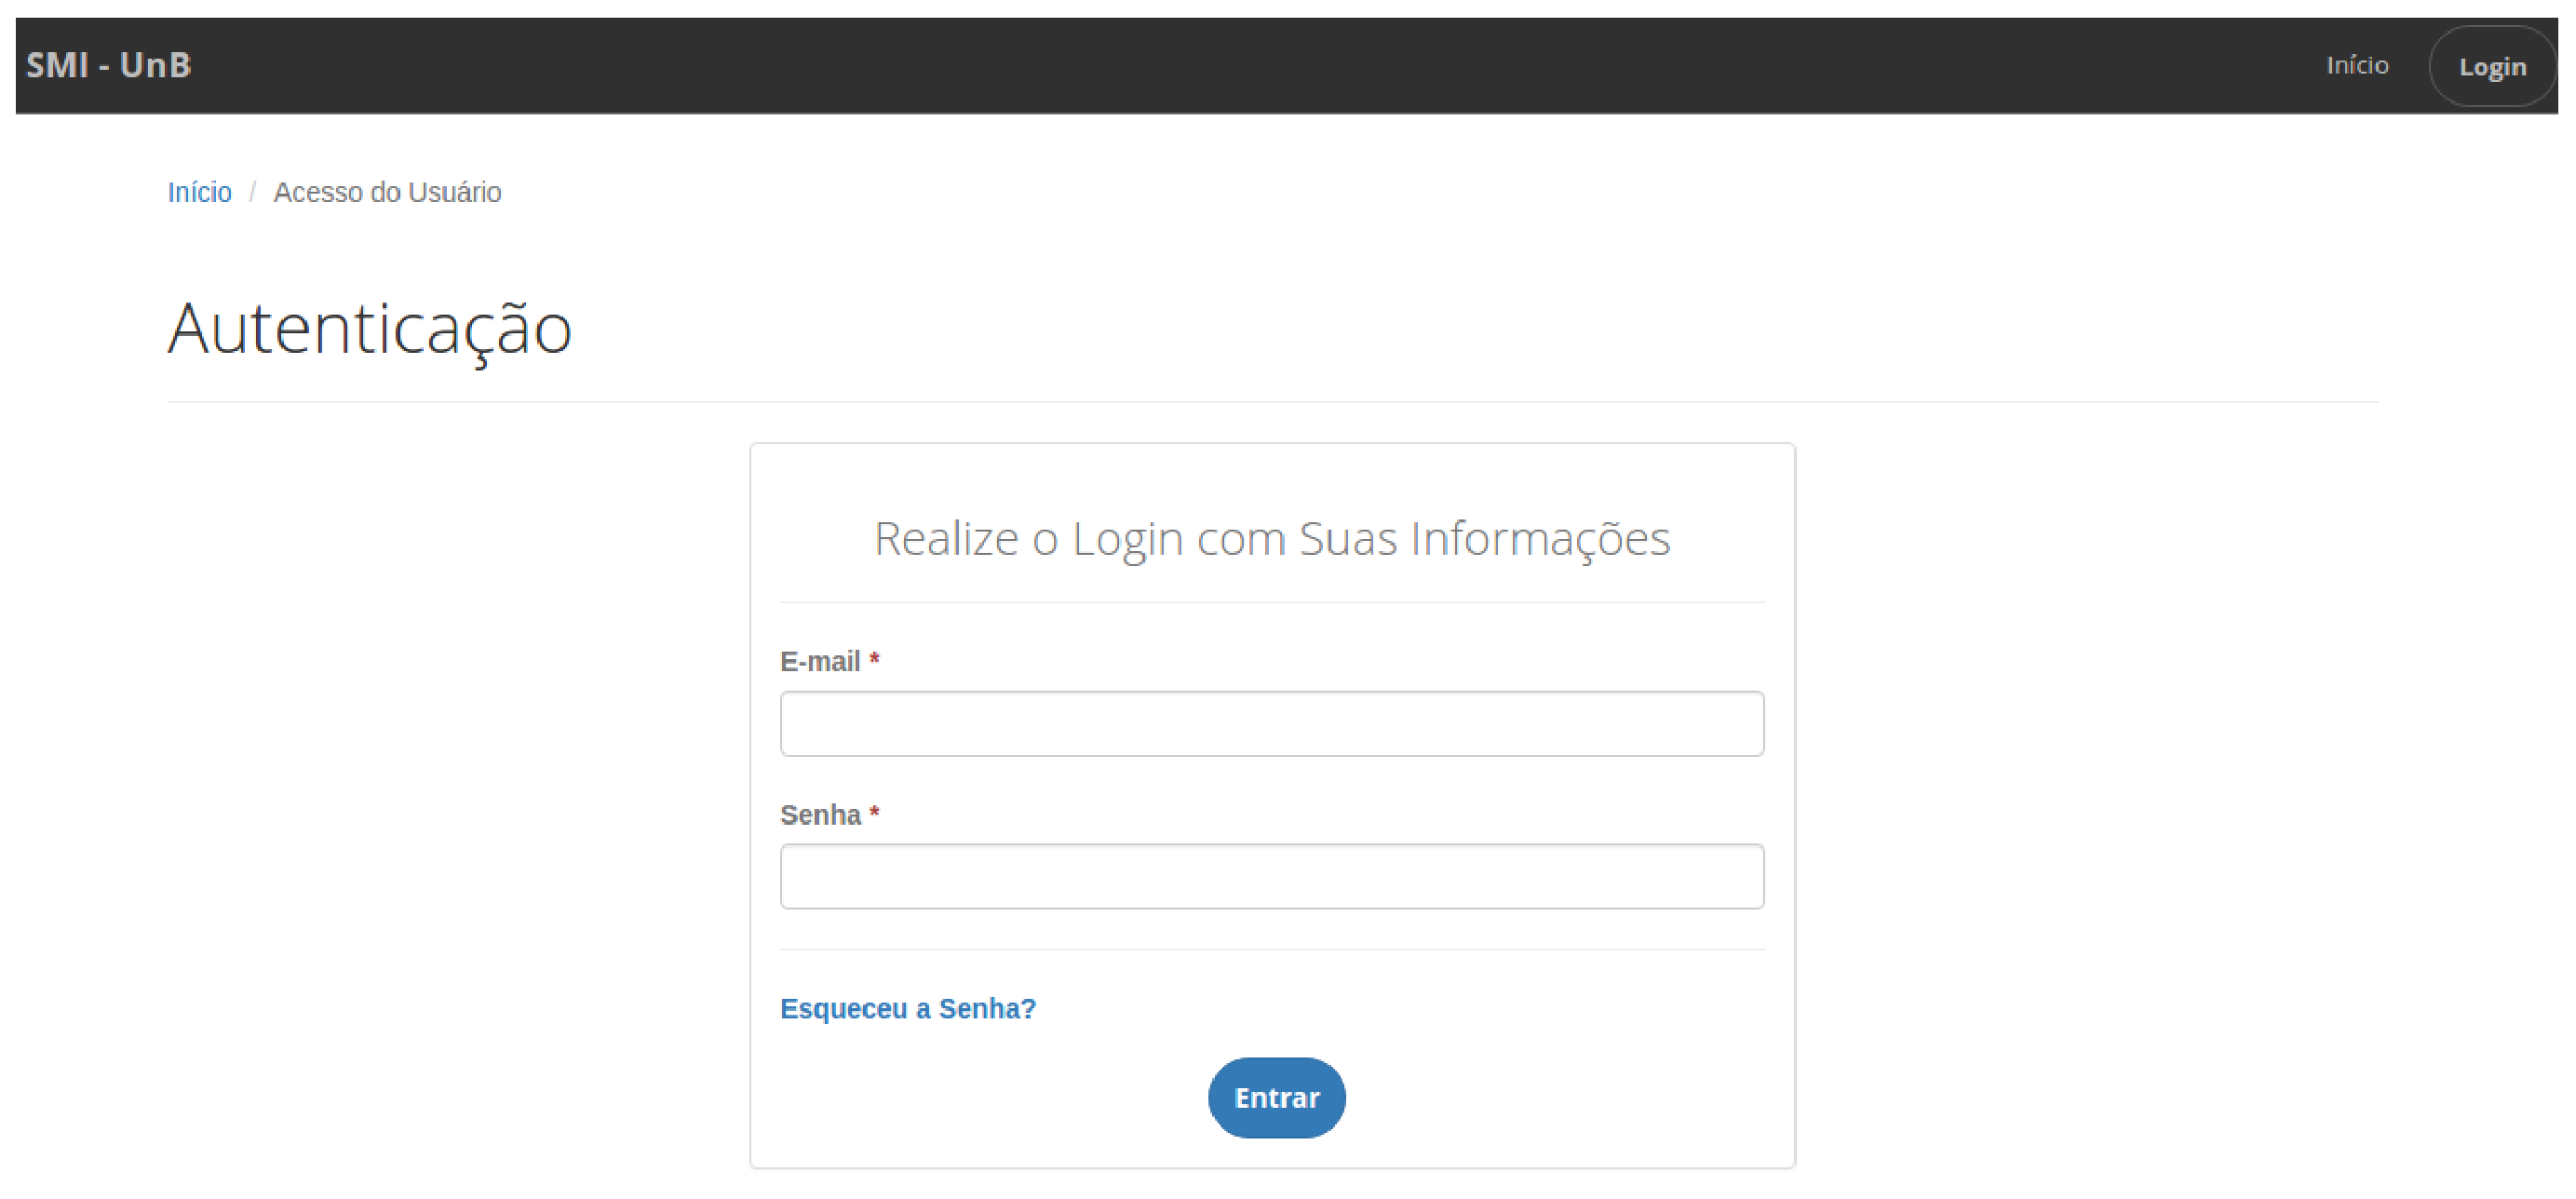
\includegraphics[keepaspectratio=true,scale=0.35]{figuras/img1.eps}
    \caption{Página de autenticação.}
    \label{img1}
\end{figure}

\begin{figure}[!htpb]
    \centering
    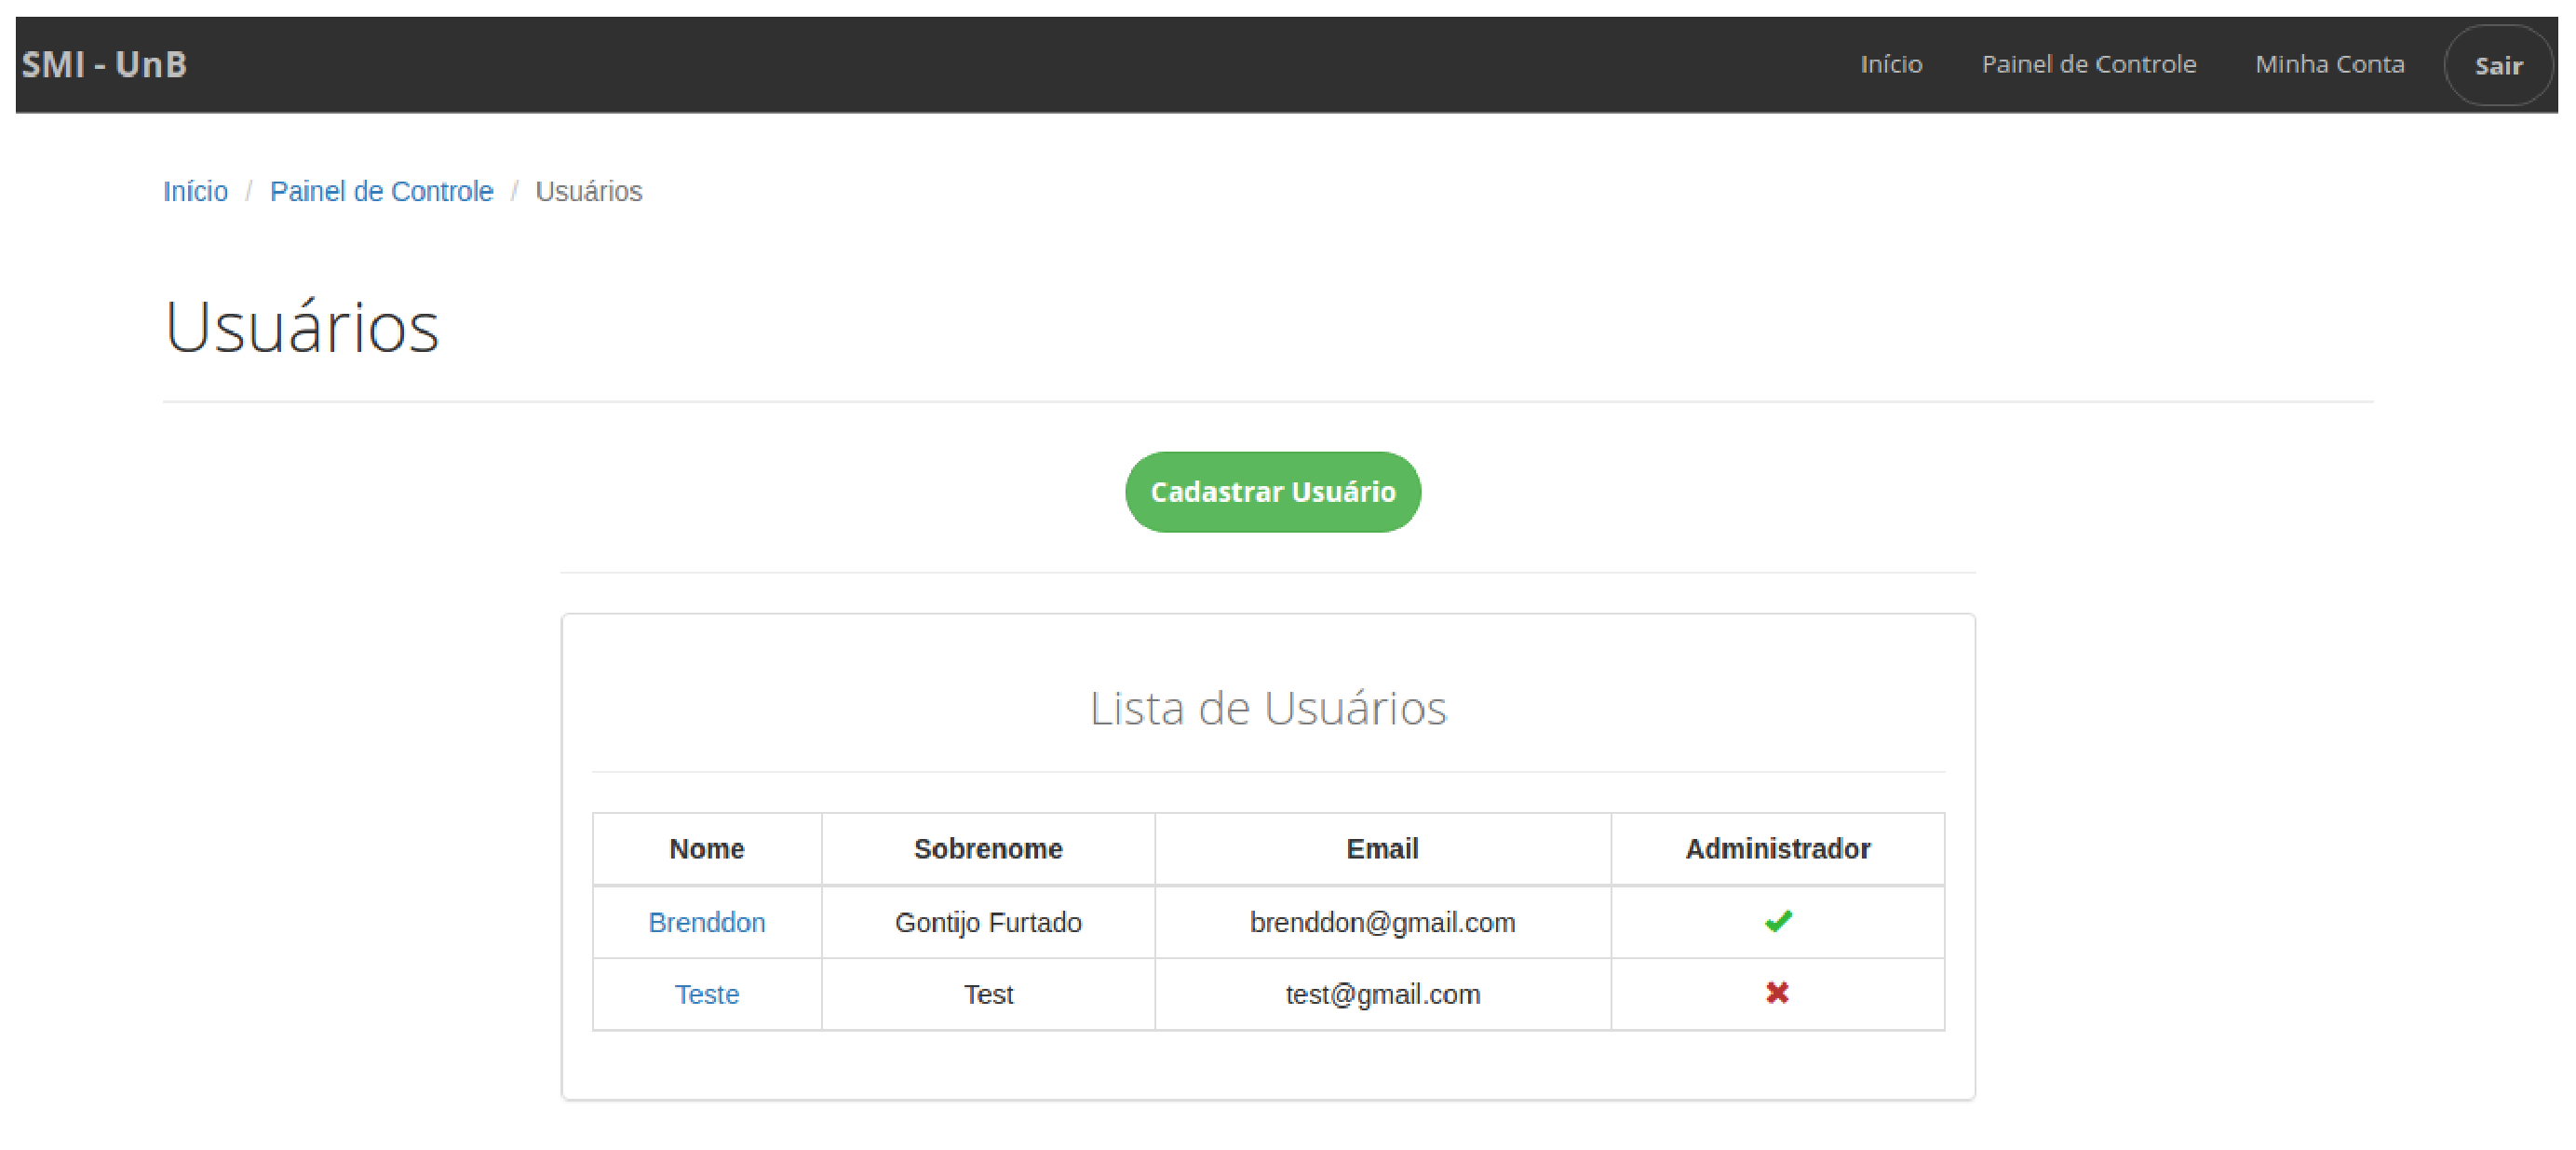
\includegraphics[keepaspectratio=true,scale=0.35]{figuras/img2.eps}
    \caption{Página de usuários.}
    \label{img2}
\end{figure}

\begin{figure}[!htpb]
    \centering
    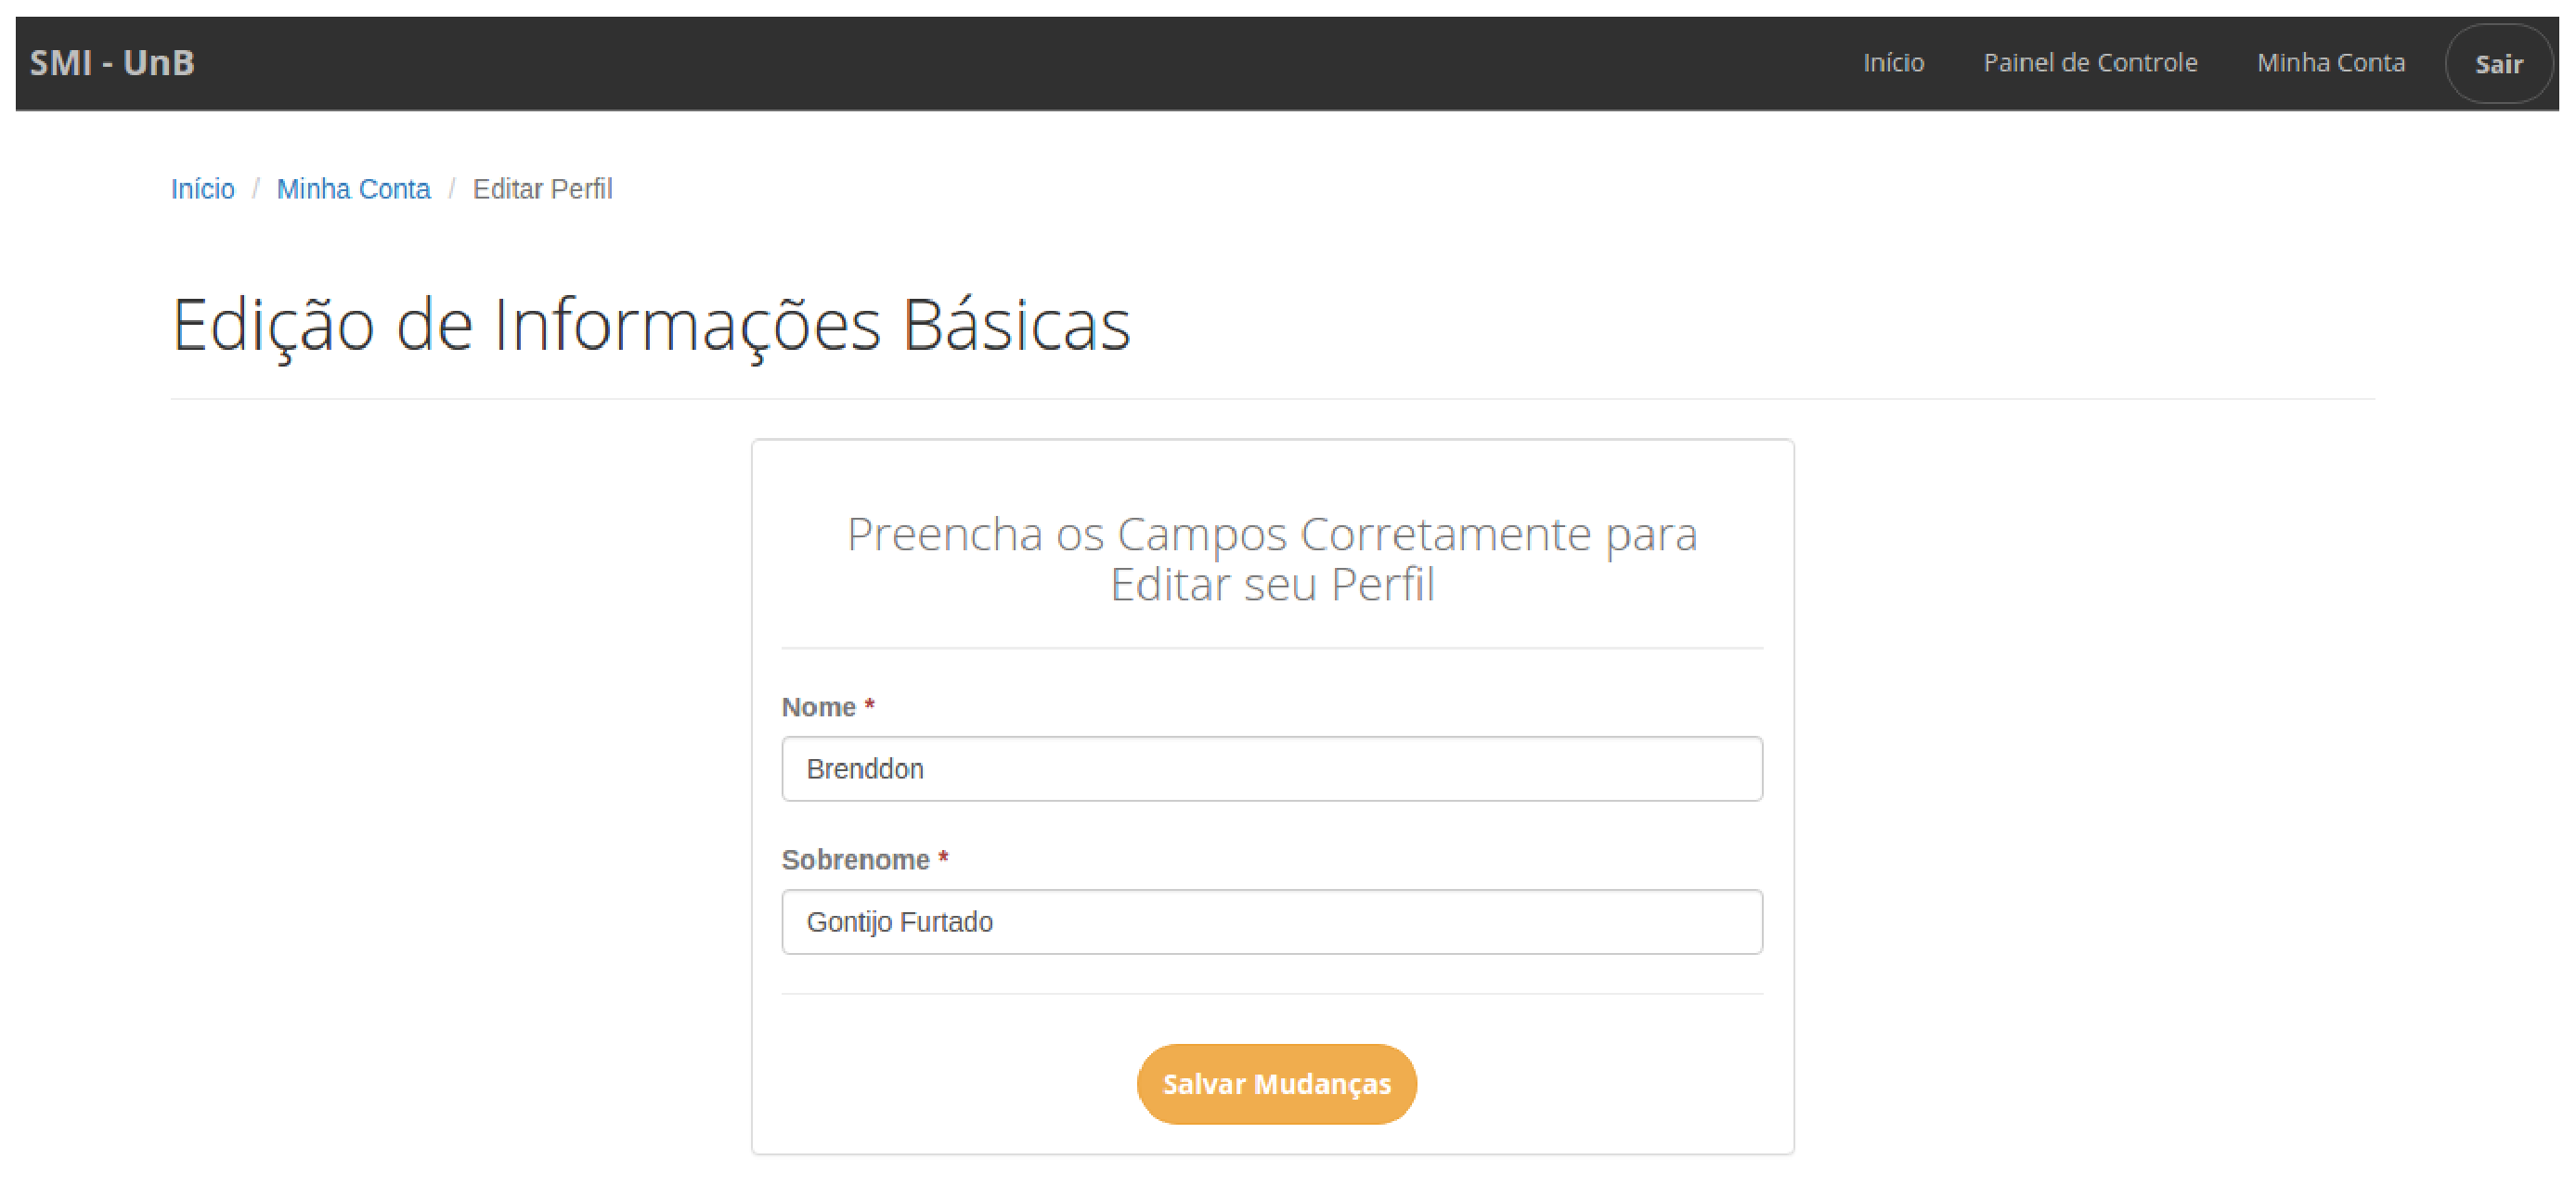
\includegraphics[keepaspectratio=true,scale=0.35]{figuras/img5.eps}
    \caption{Página de edição das informações básicas da conta.}
    \label{img5}
\end{figure}

\begin{figure}[!htpb]
    \centering
    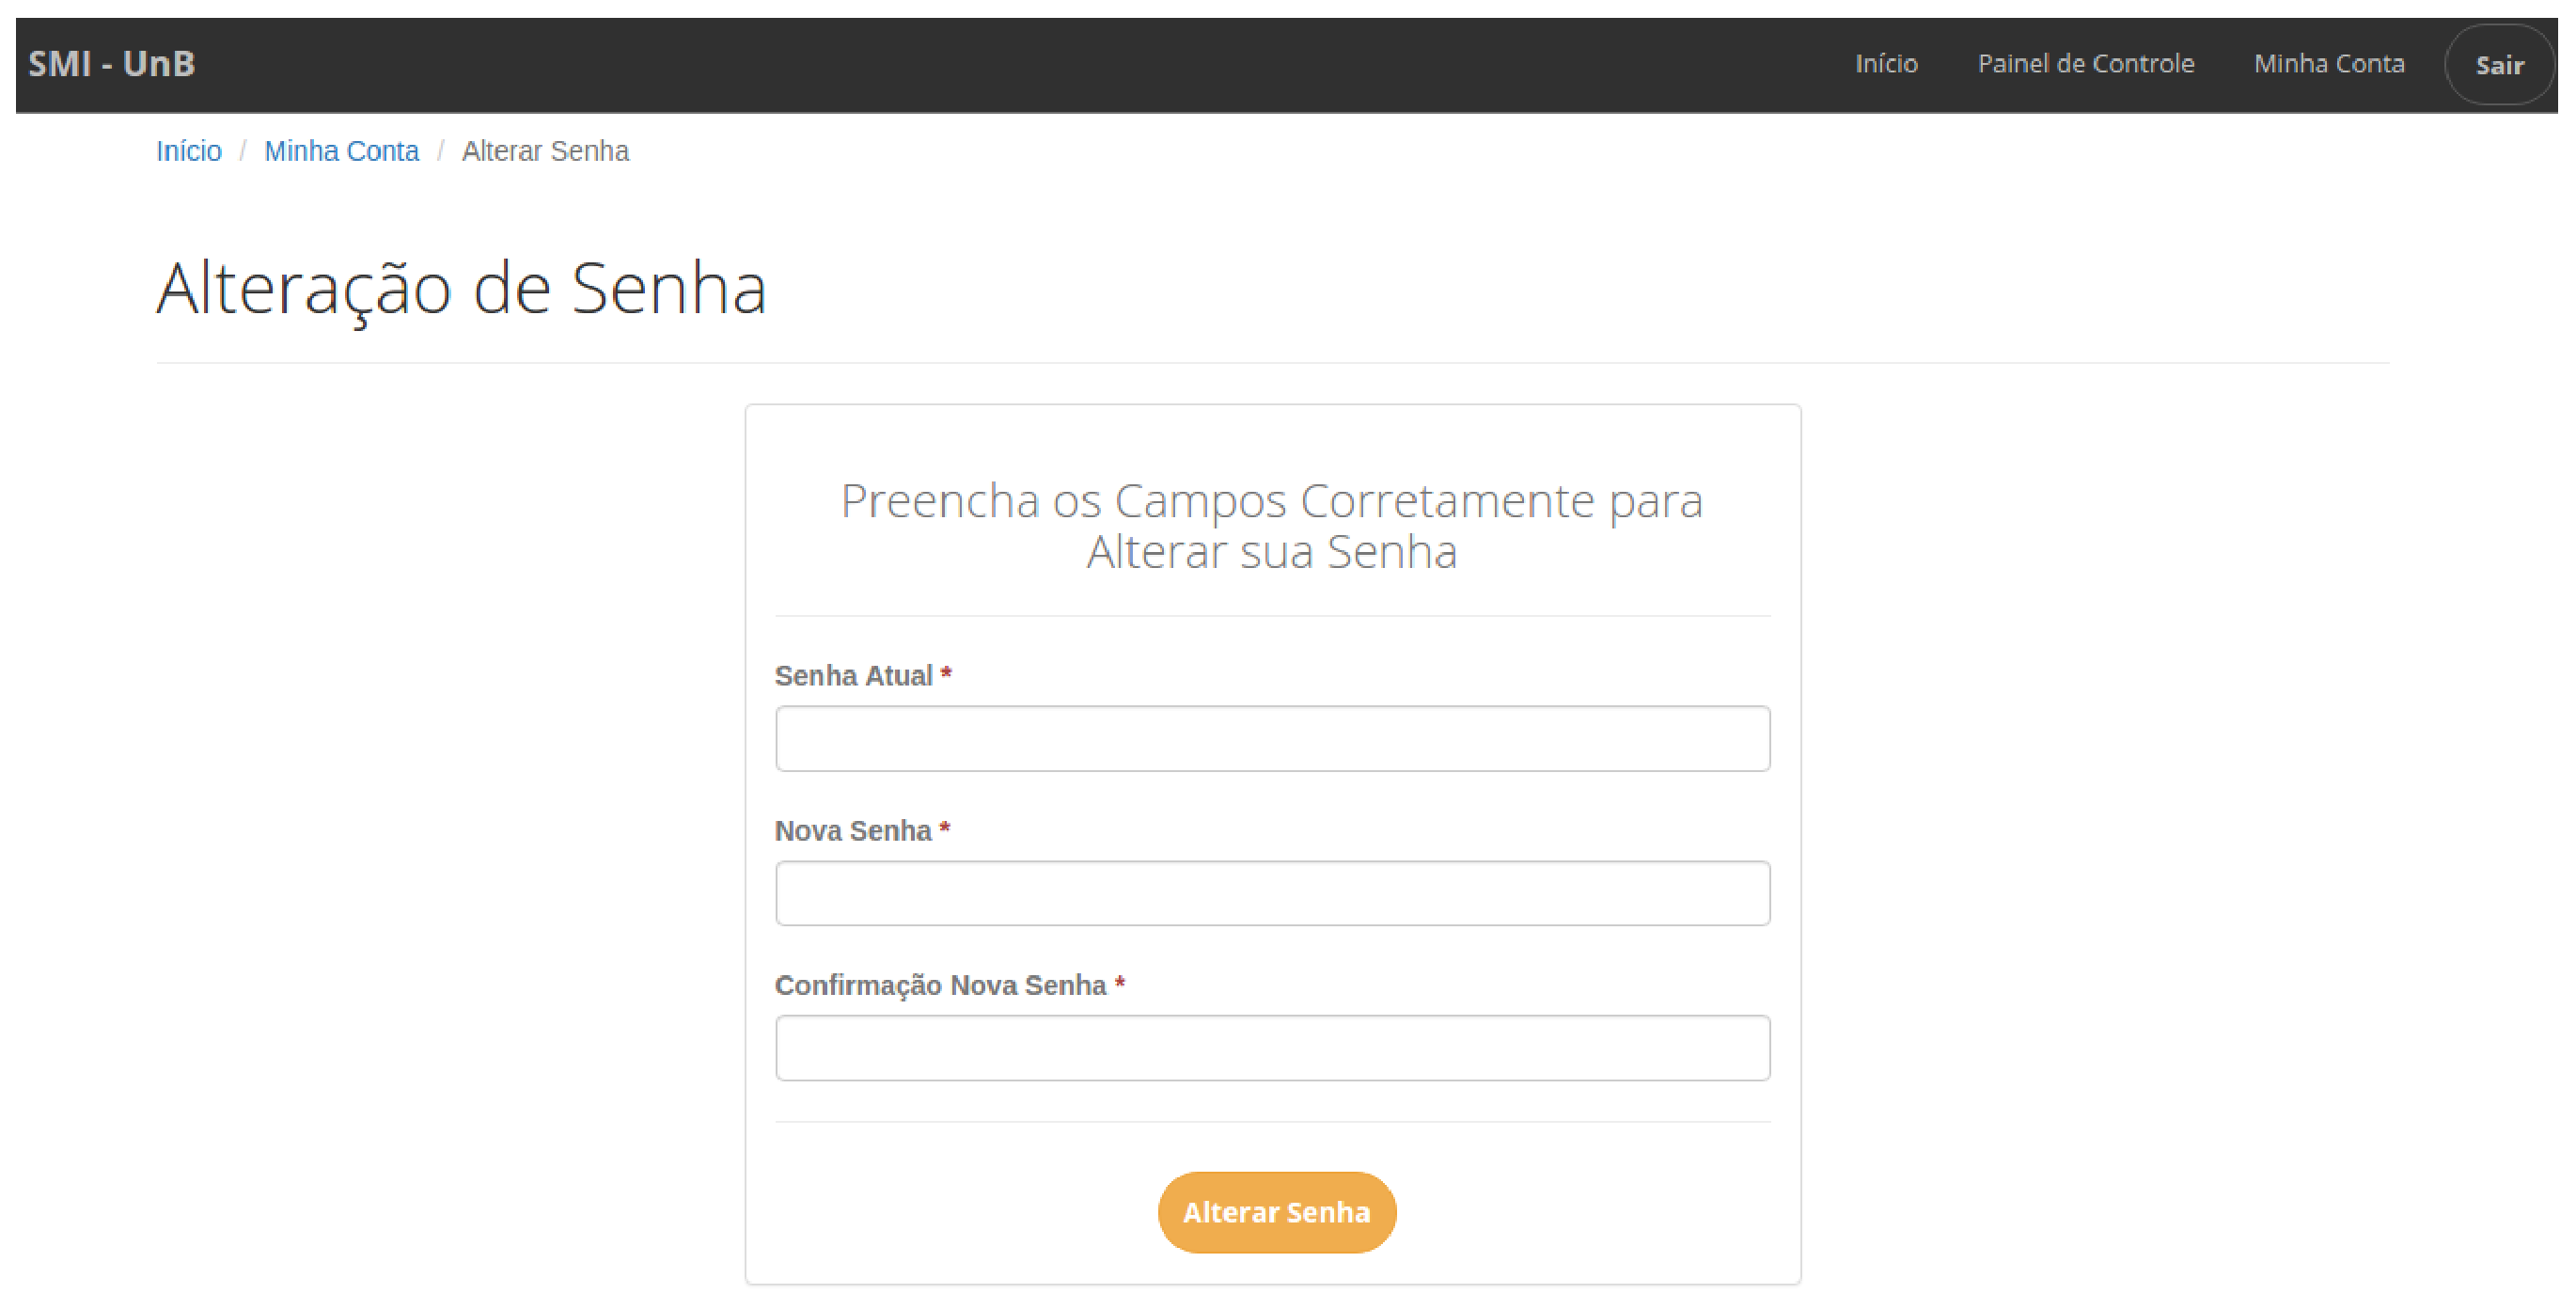
\includegraphics[keepaspectratio=true,scale=0.35]{figuras/img6.eps}
    \caption{Página de alteração de senha.}
    \label{img6}
\end{figure}

\begin{figure}[!htpb]
    \centering
    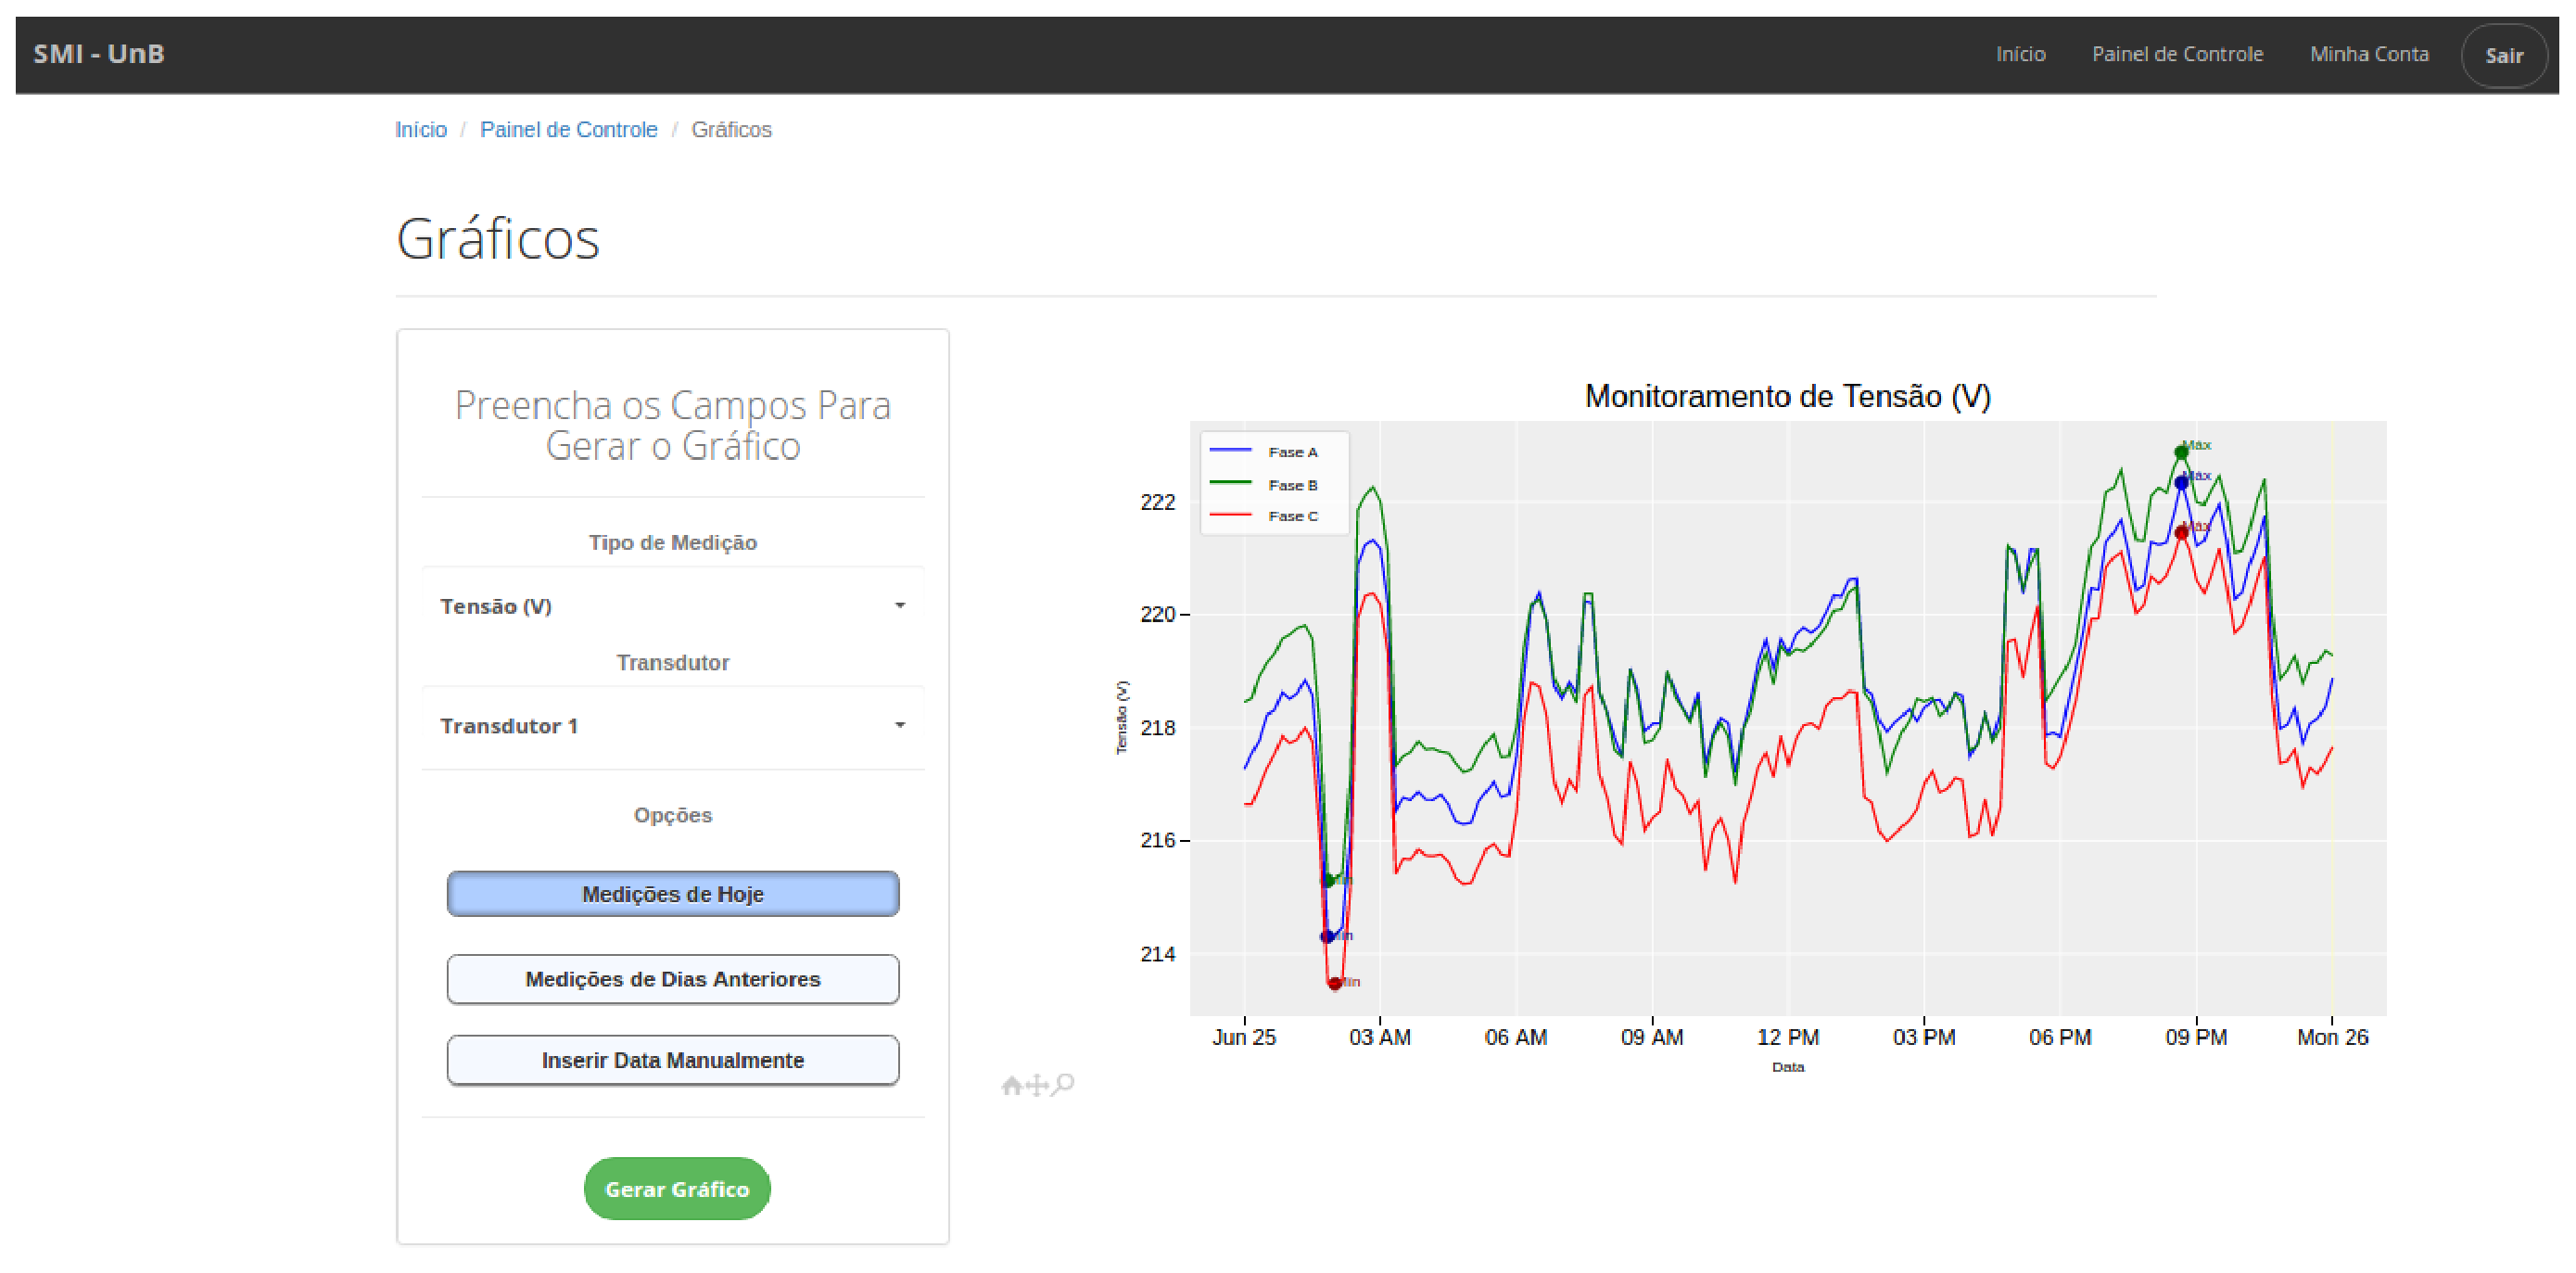
\includegraphics[keepaspectratio=true,scale=0.35]{figuras/img15.eps}
    \caption{Página de gráficos.}
    \label{img15}
\end{figure}

\begin{figure}[!htpb]
    \centering
    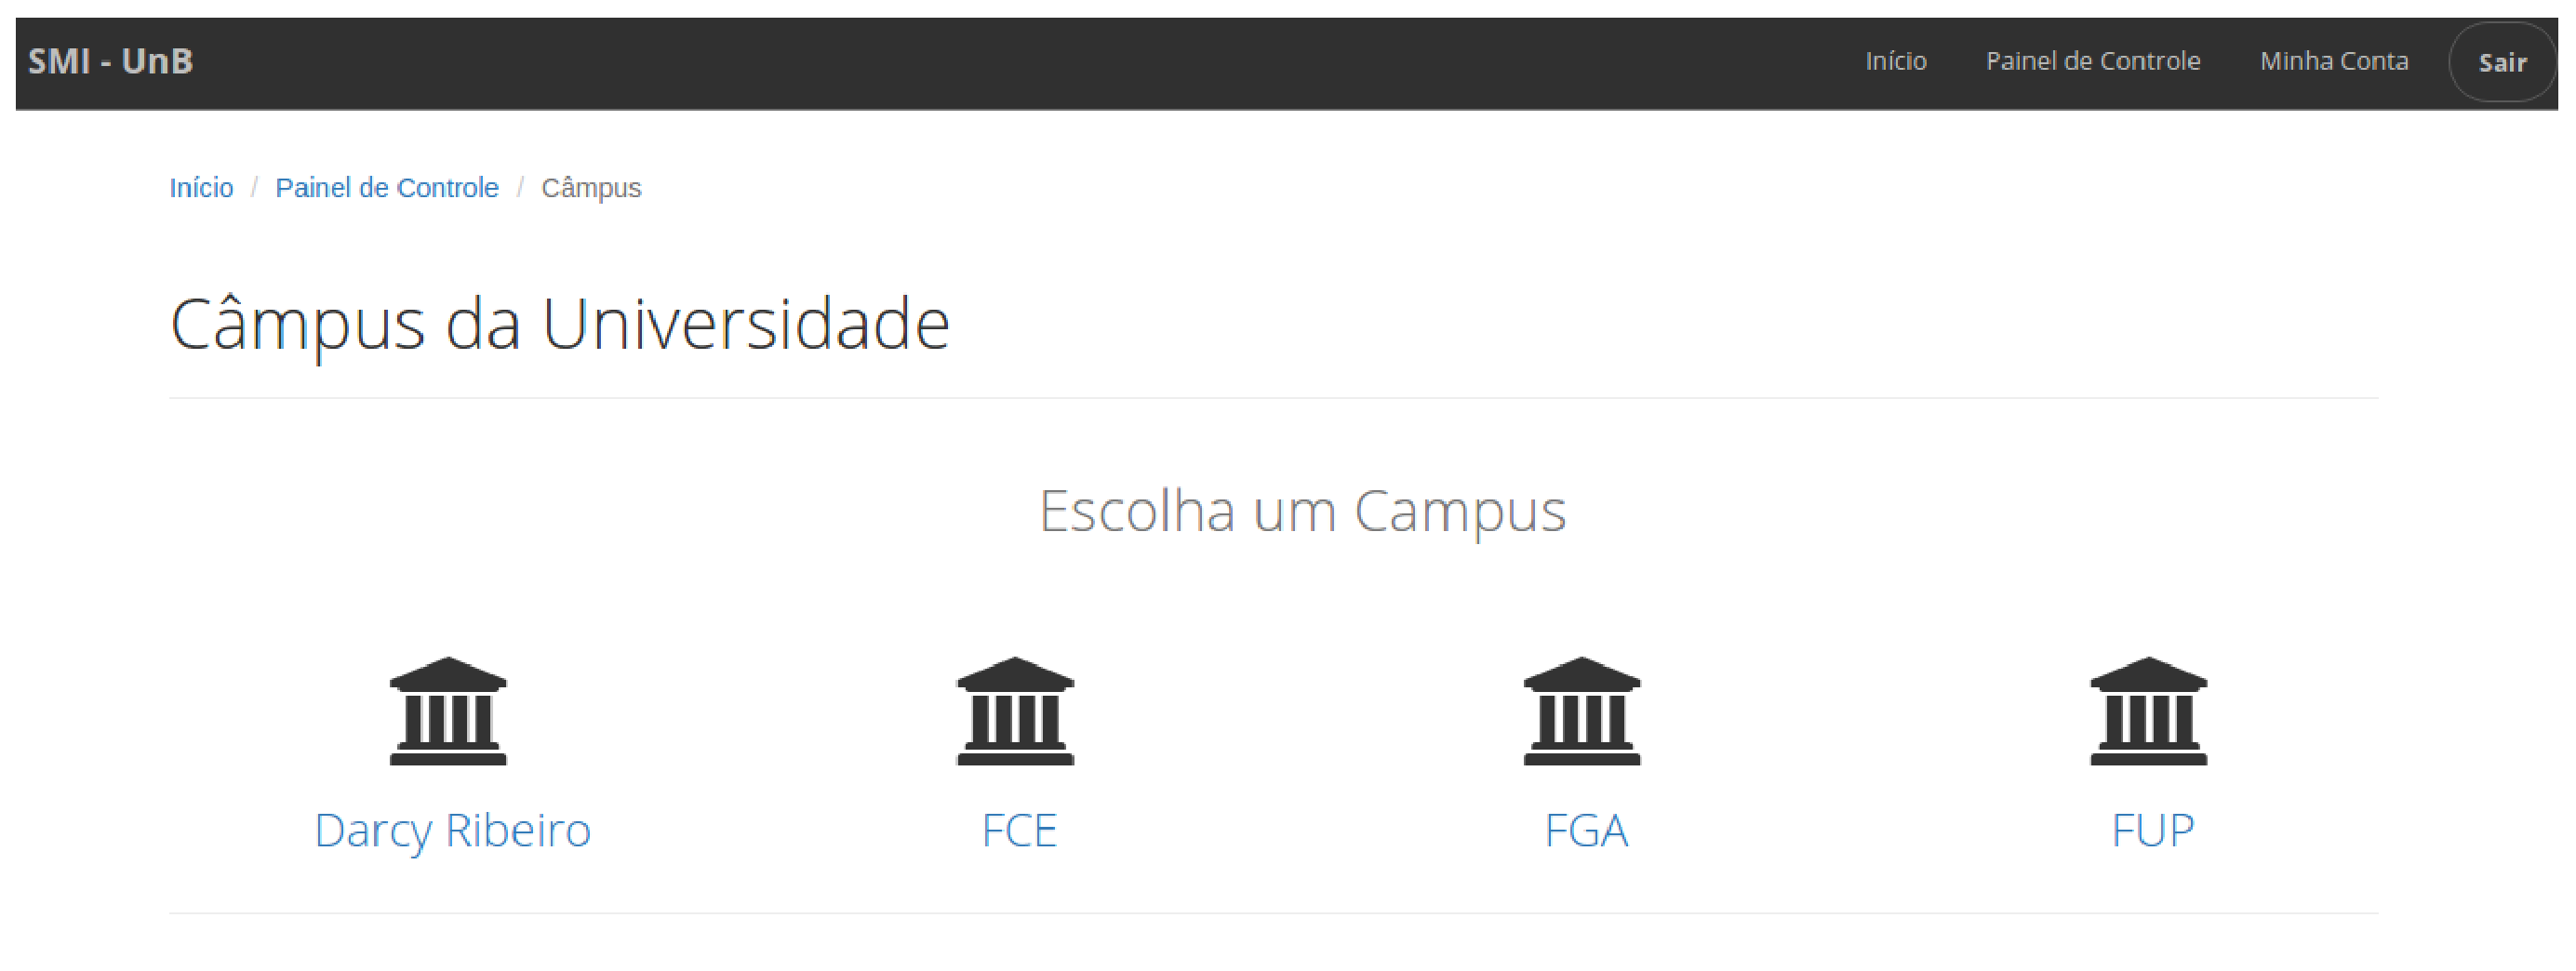
\includegraphics[keepaspectratio=true,scale=0.35]{figuras/img7.eps}
    \caption{Página dos \textit{campi} da UnB.}
    \label{img7}
\end{figure}

\begin{figure}[!htpb]
    \centering
    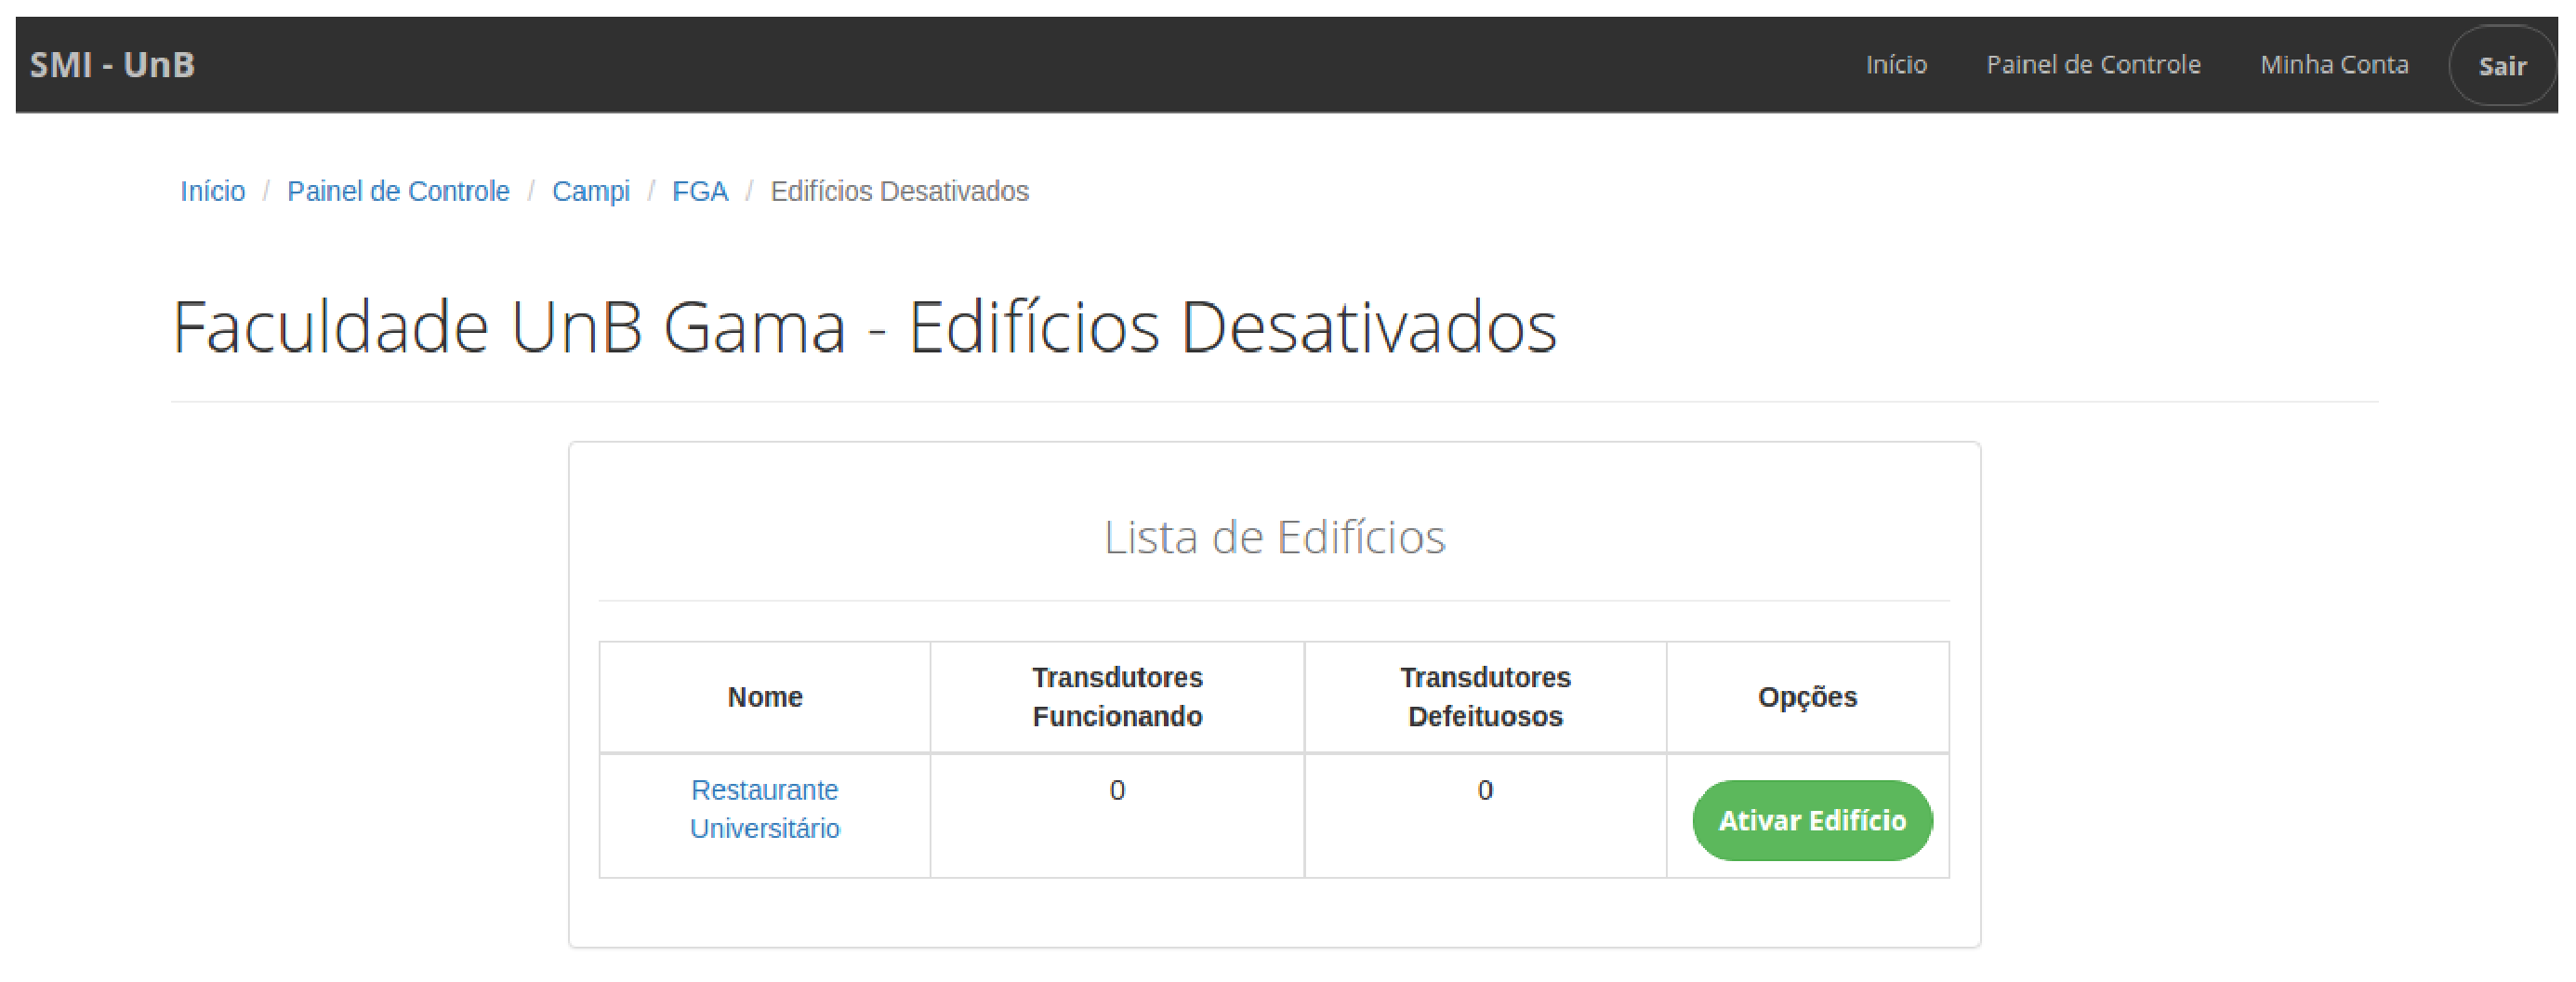
\includegraphics[keepaspectratio=true,scale=0.35]{figuras/img8.eps}
    \caption{Página de edifícios desativados em um campus.}
    \label{img8}
\end{figure}

\begin{figure}[!htpb]
    \centering
    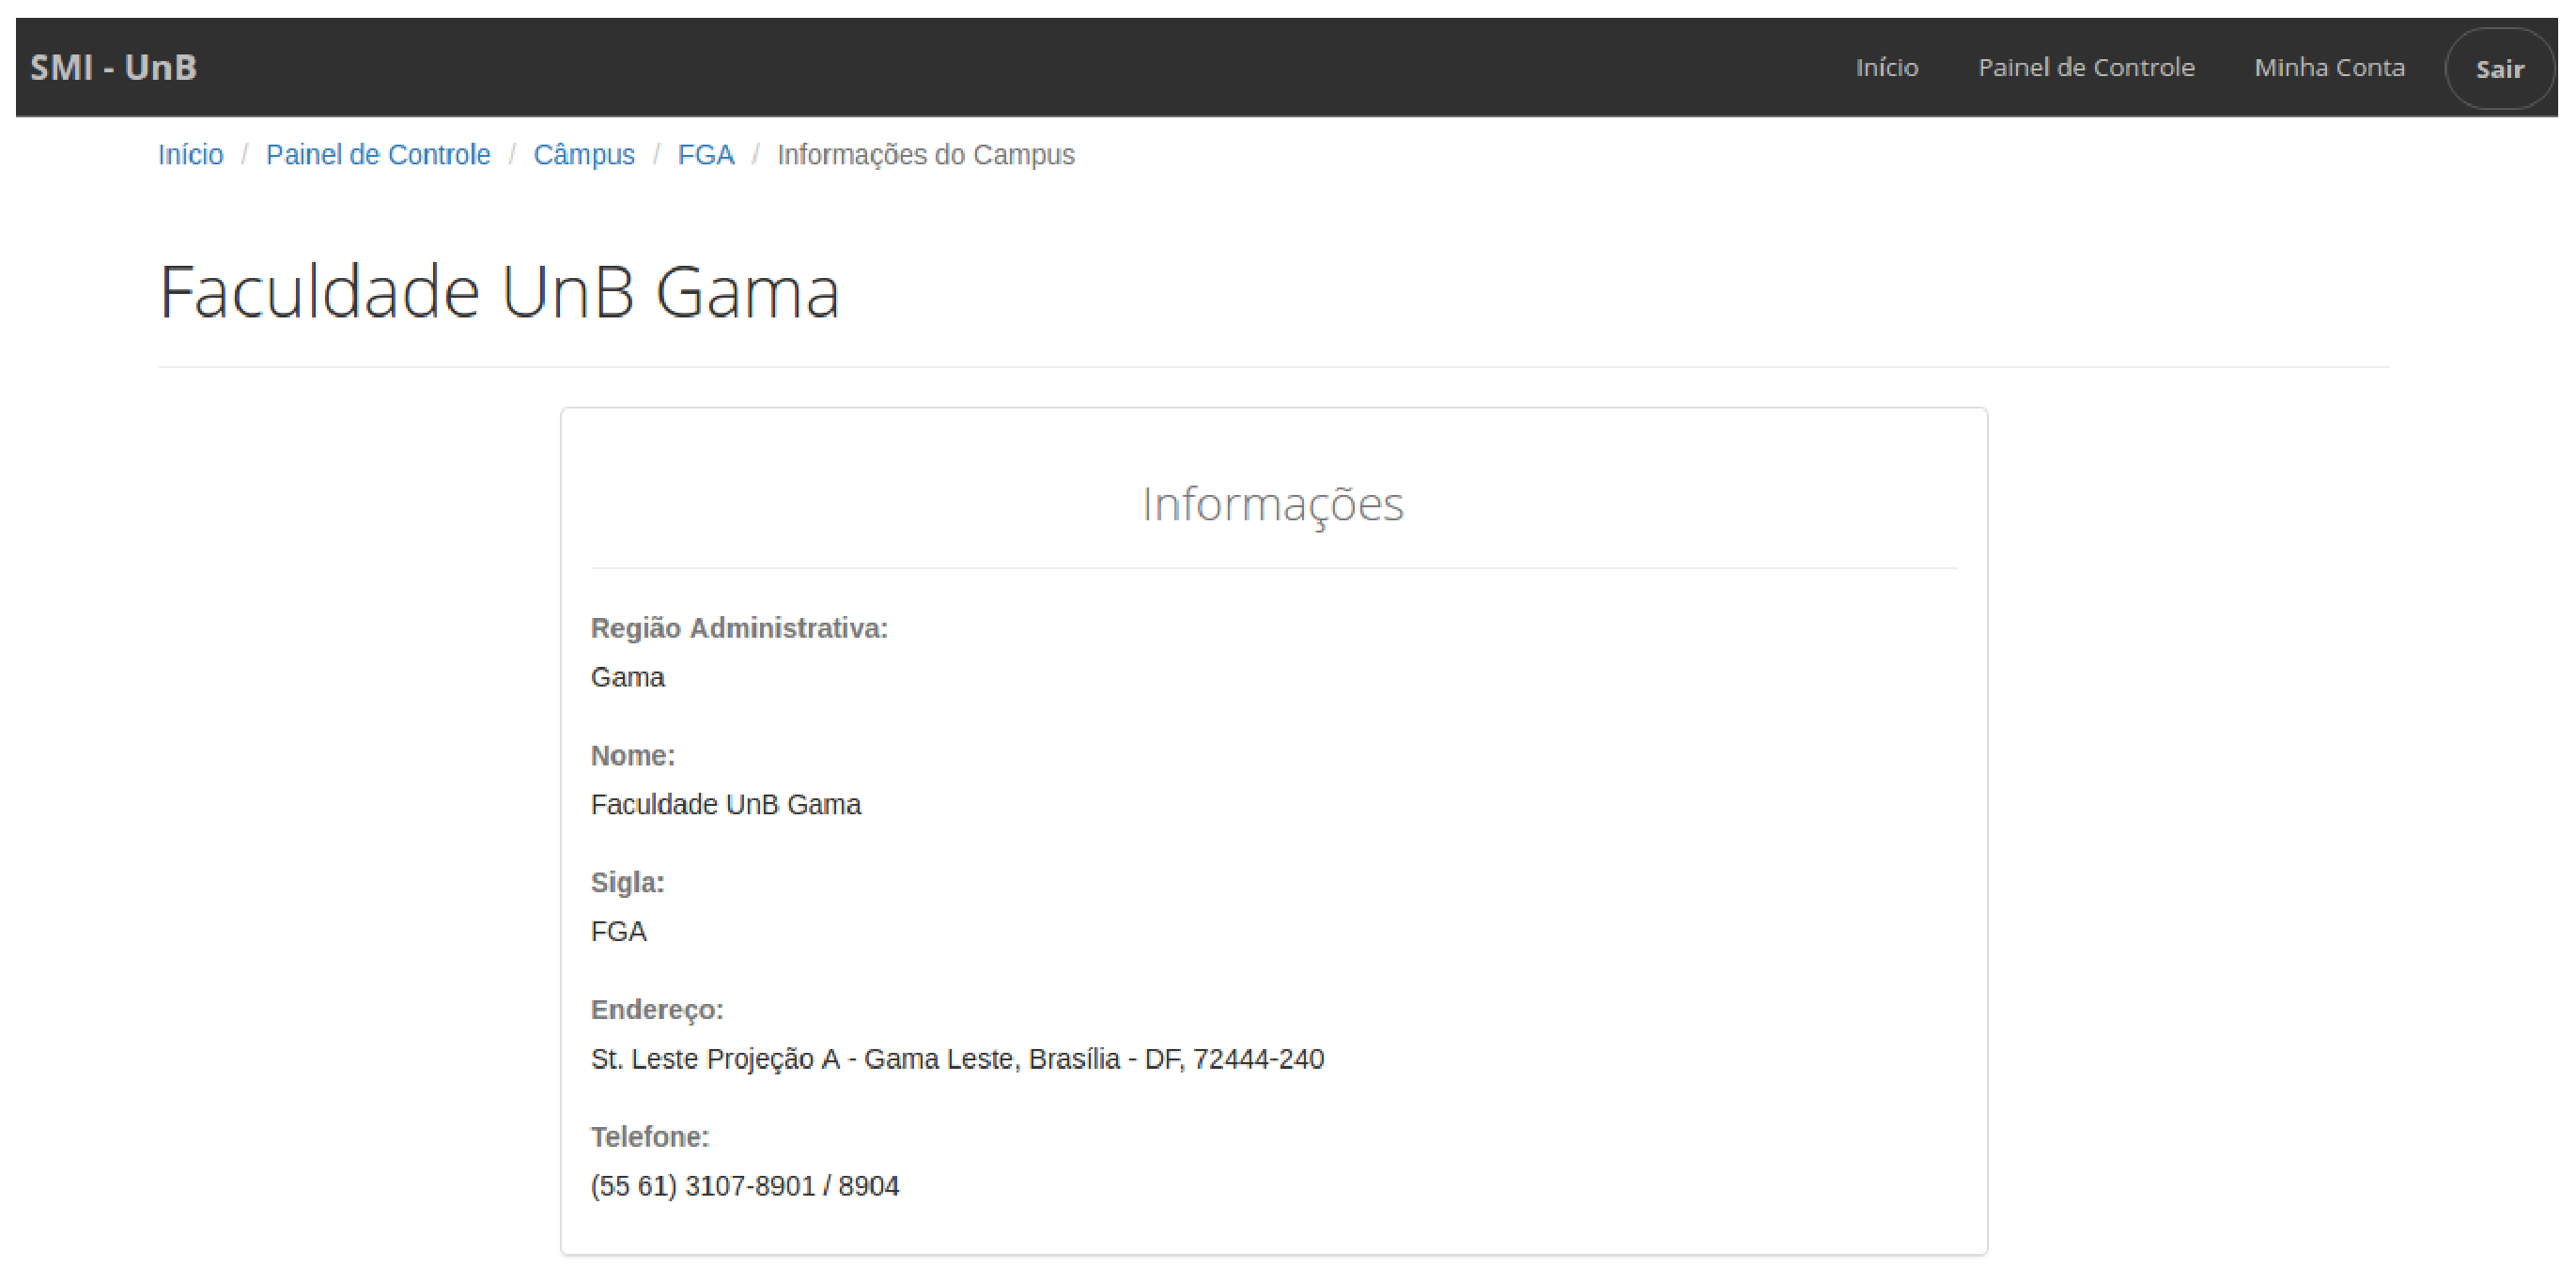
\includegraphics[keepaspectratio=true,scale=0.35]{figuras/img9.eps}
    \caption{Página de informações de em um campus.}
    \label{img9}
\end{figure}

\begin{figure}[!htpb]
    \centering
    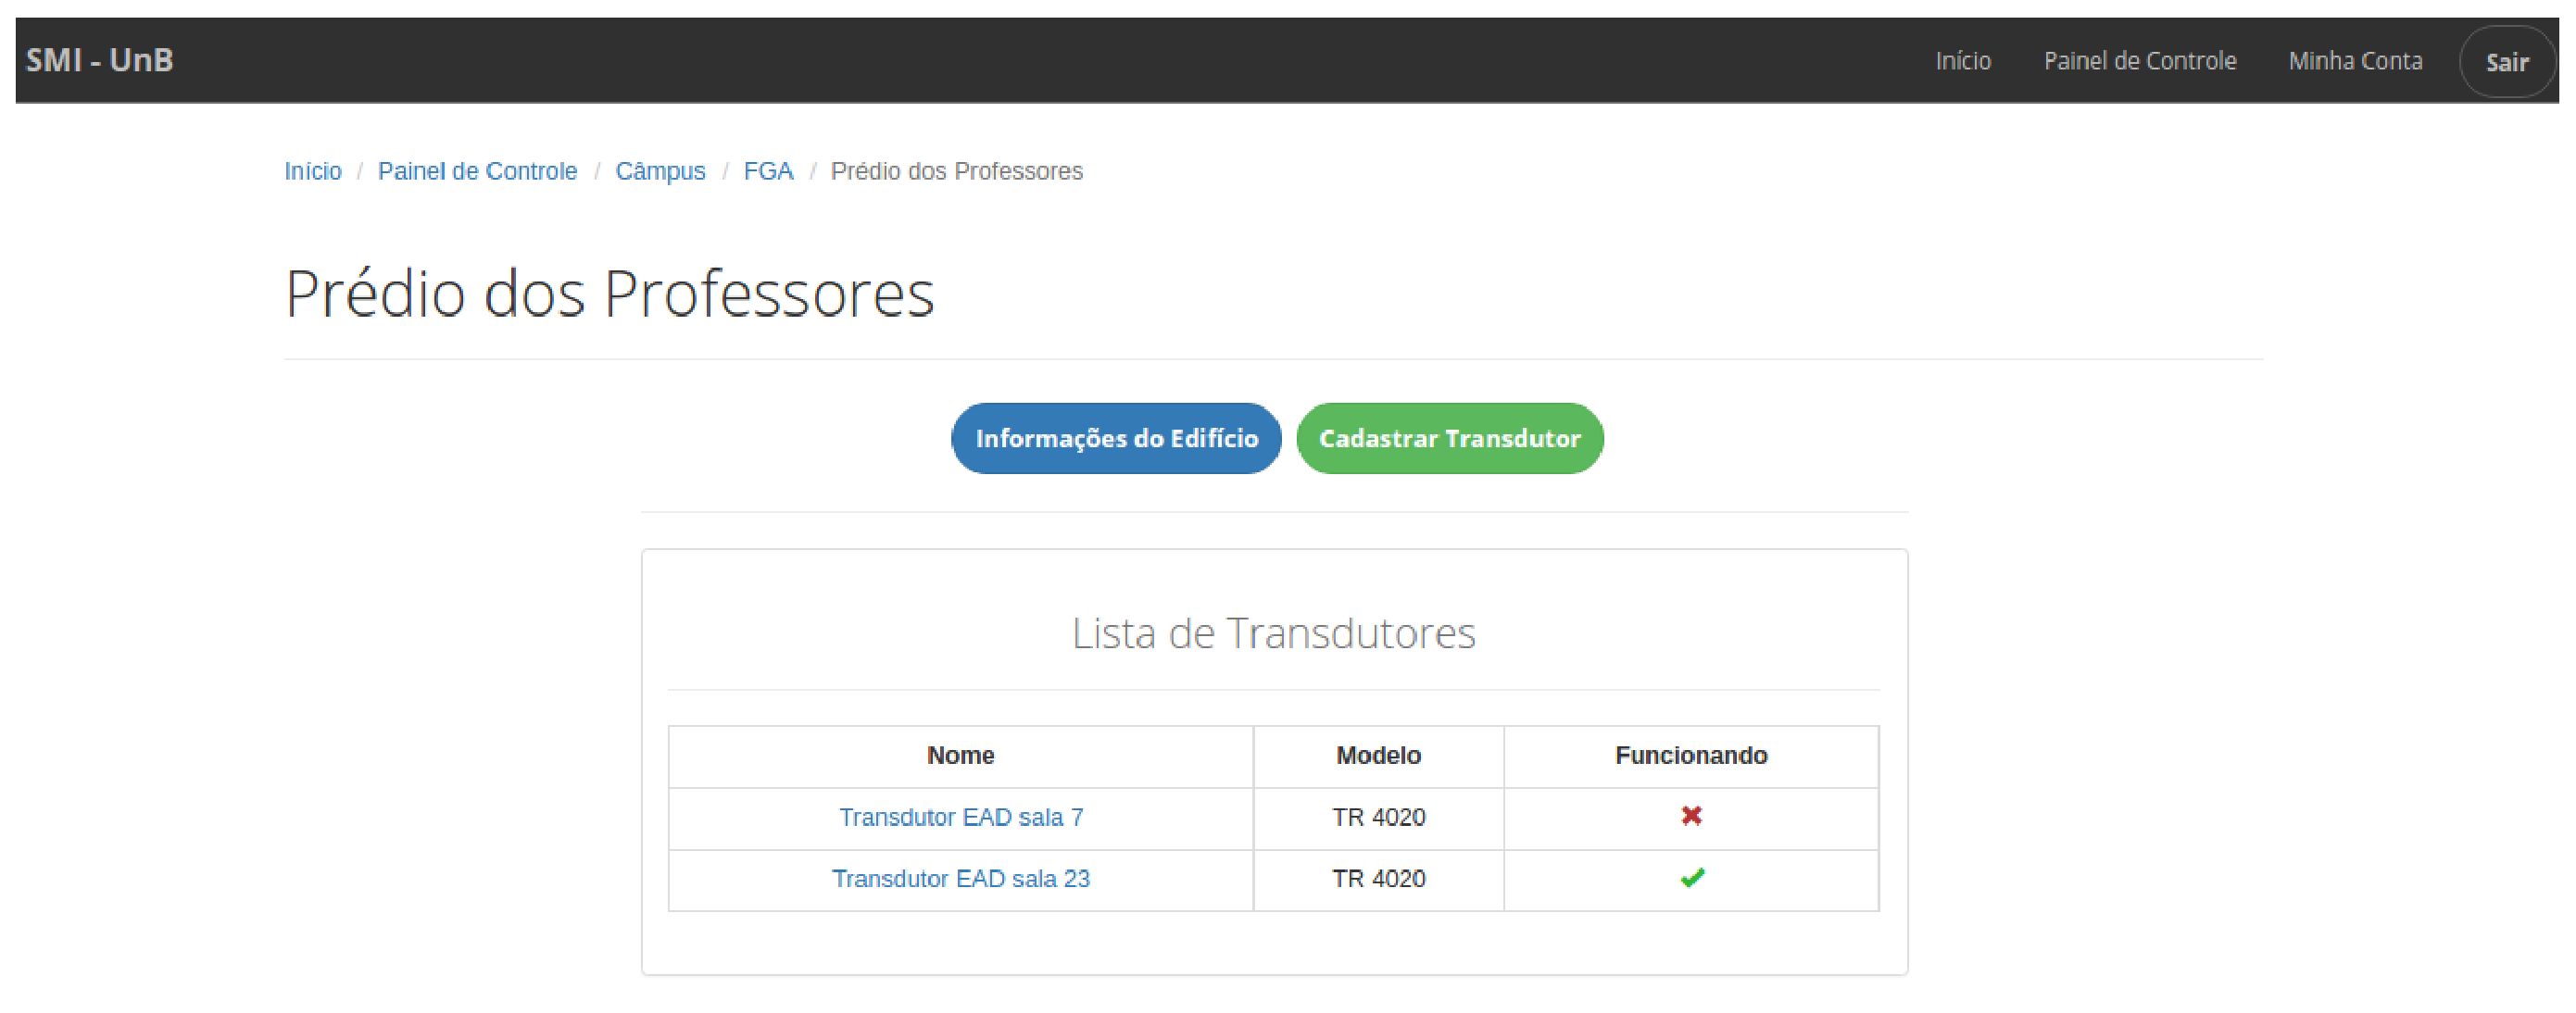
\includegraphics[keepaspectratio=true,scale=0.35]{figuras/img11.eps}
    \caption{Página principal de um edifício.}
    \label{img11}
\end{figure}

\begin{figure}[!htpb]
    \centering
    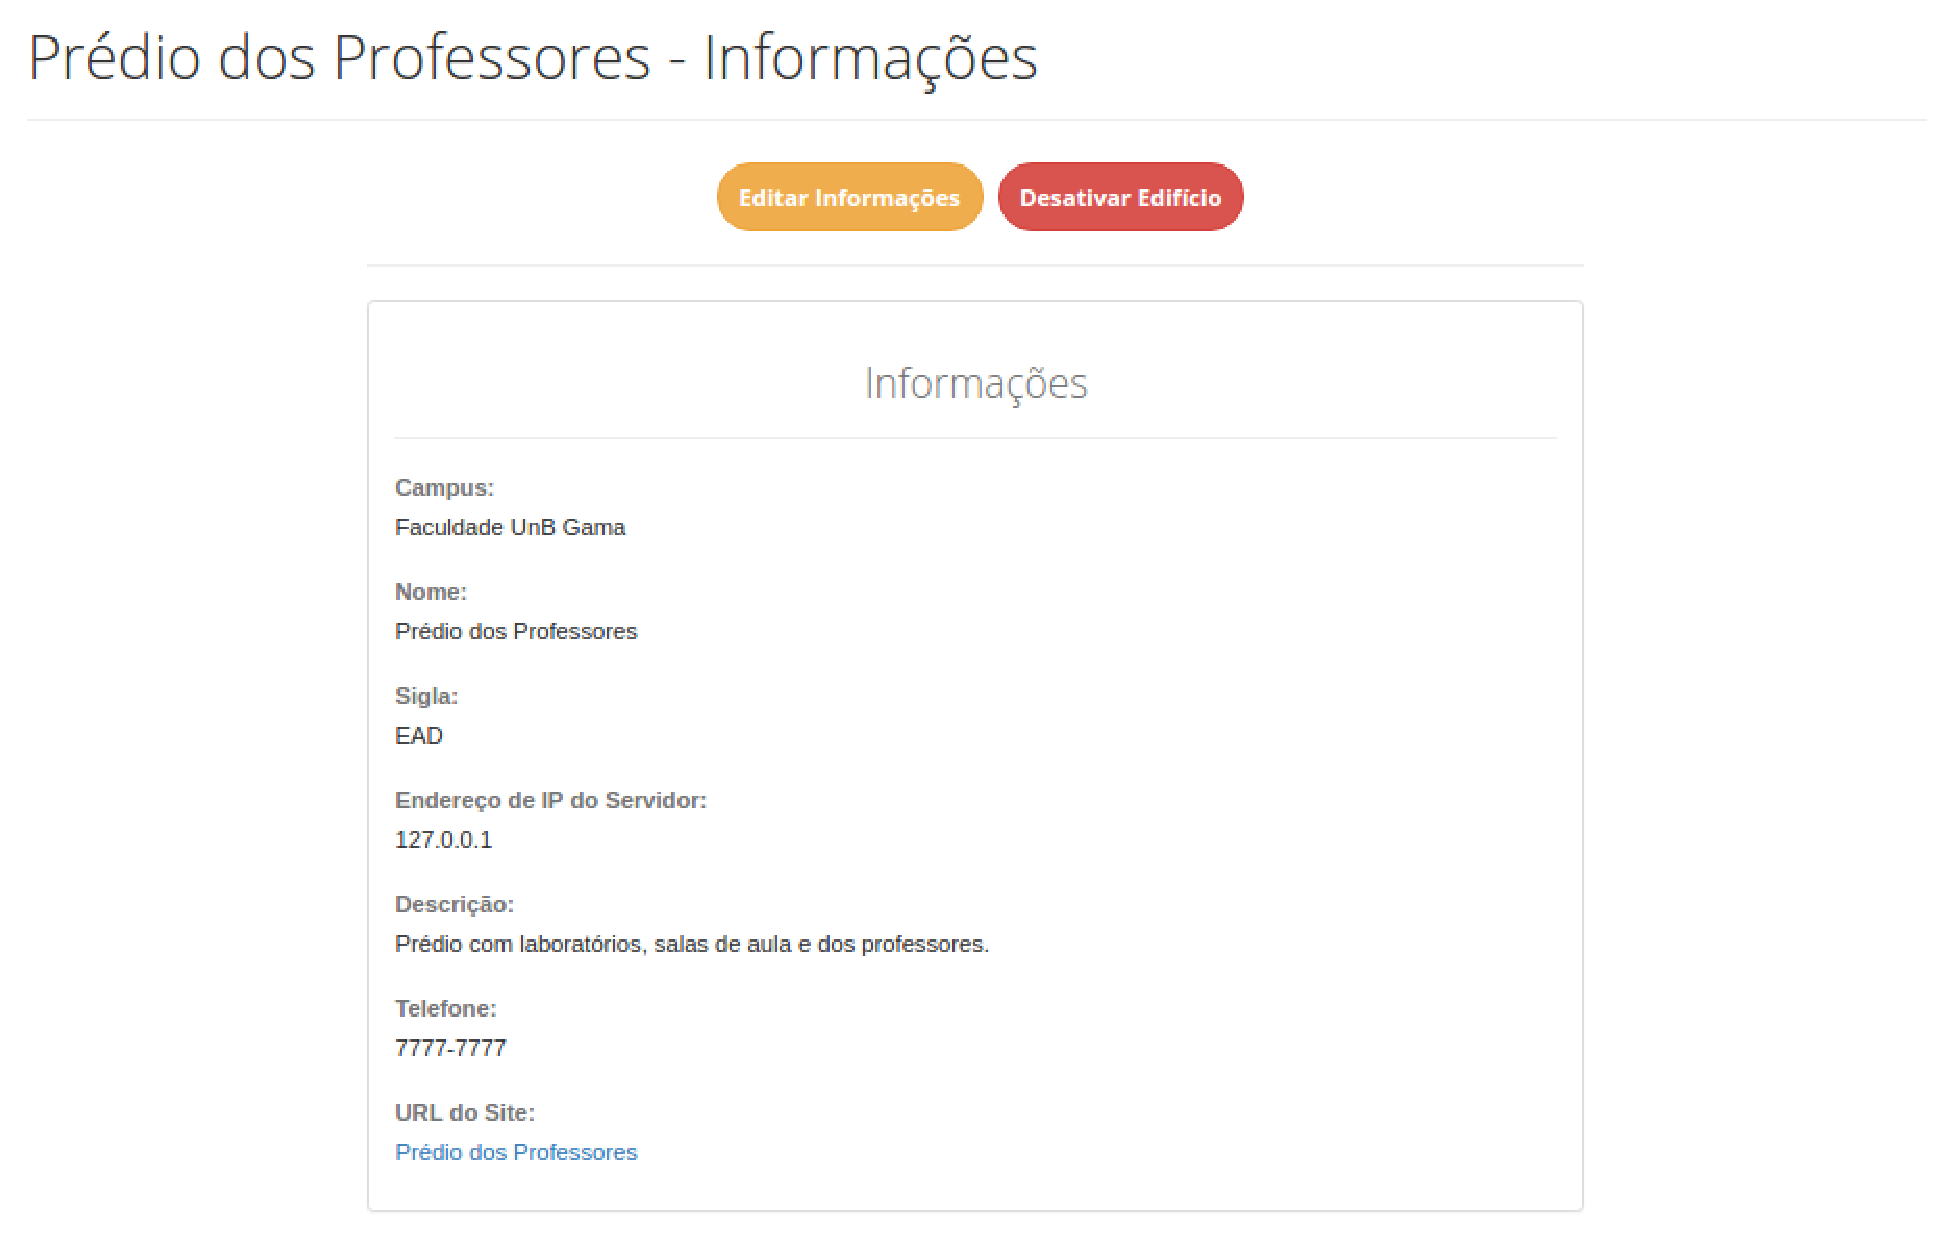
\includegraphics[keepaspectratio=true,scale=0.55]{figuras/img12.eps}
    \caption{Informações de um edifício.}
    \label{img12}
\end{figure}

\begin{figure}[!htpb]
    \centering
    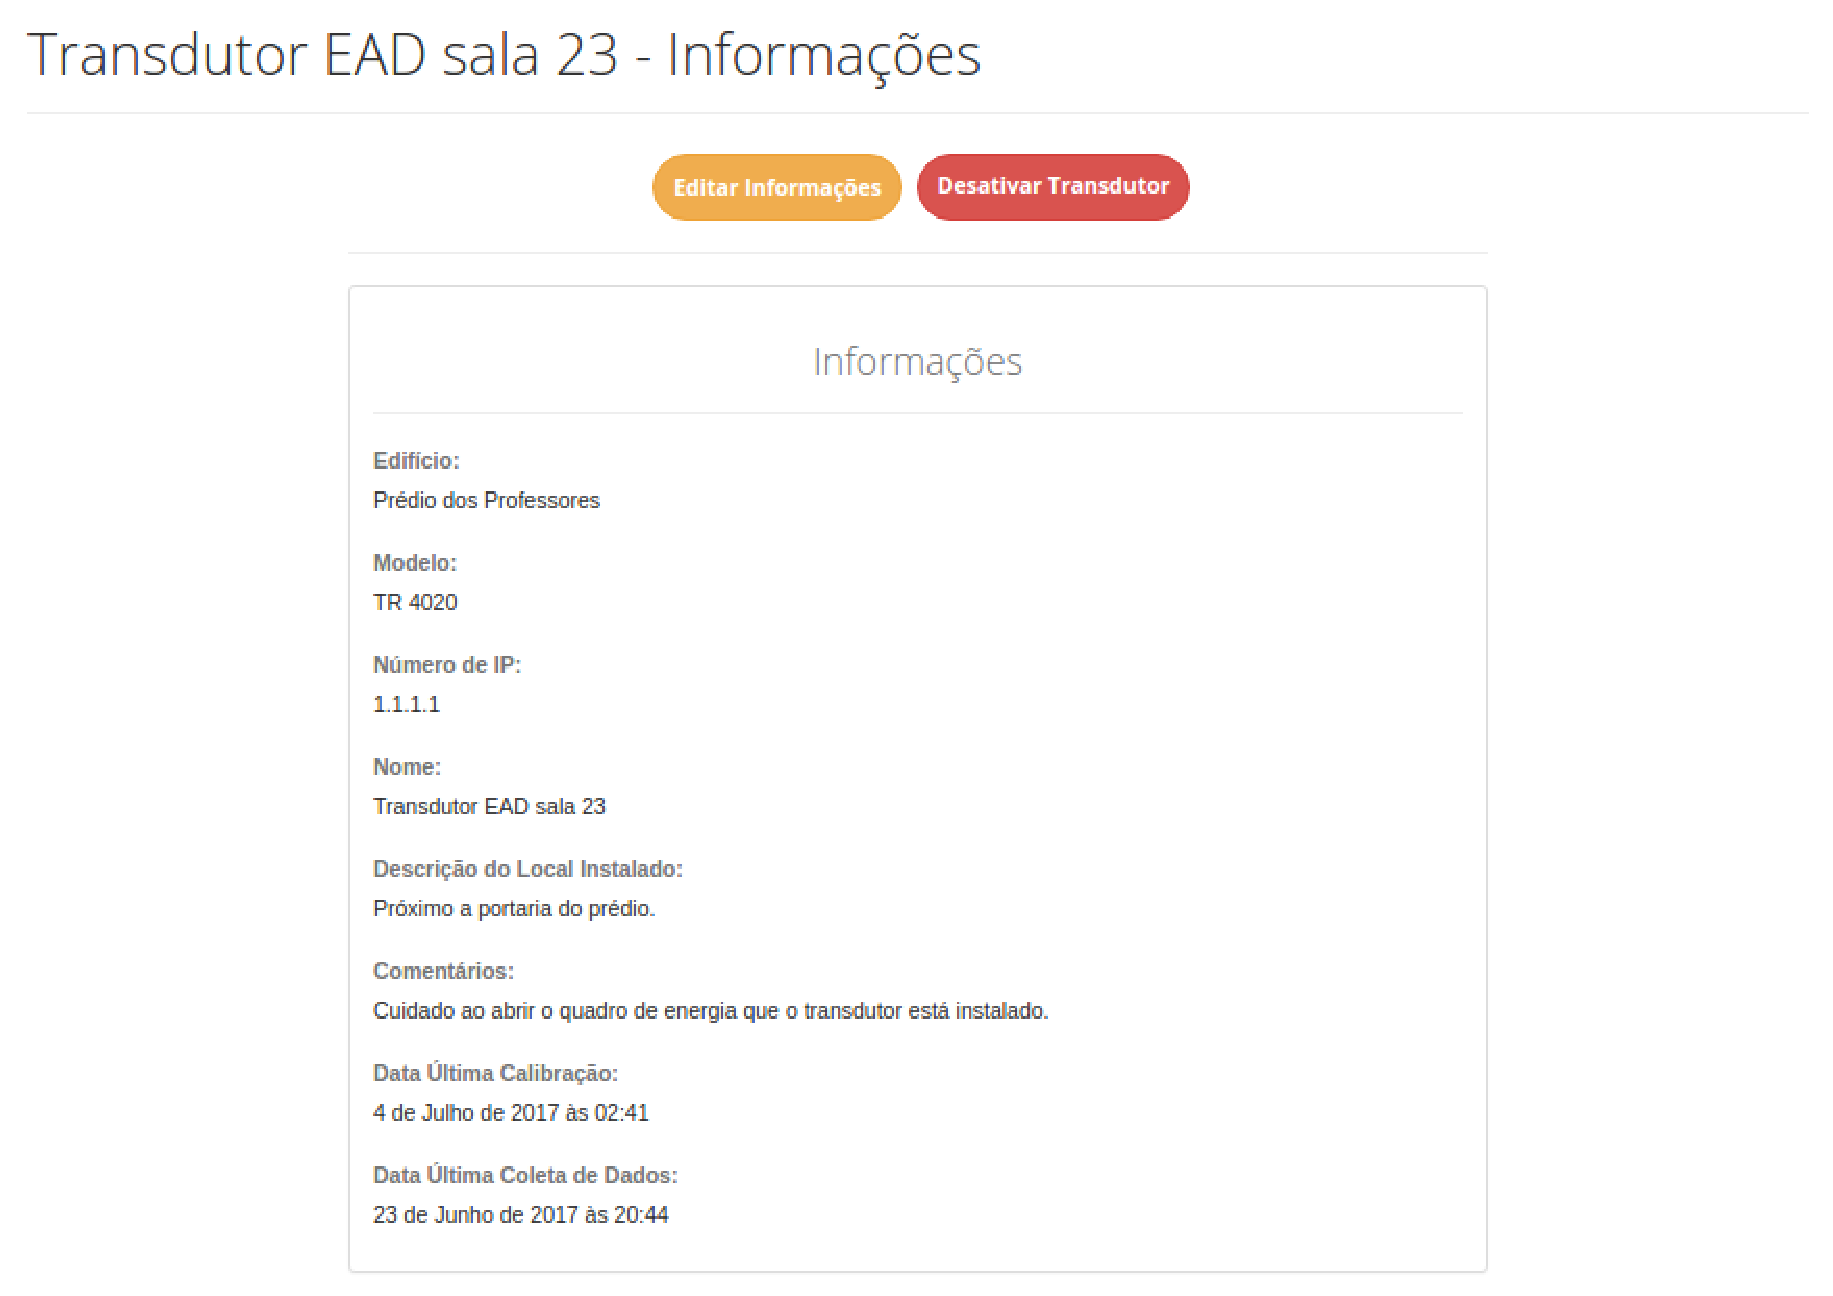
\includegraphics[keepaspectratio=true,scale=0.6]{figuras/img13.eps}
    \caption{Informações de um transdutor.}
    \label{img13}
\end{figure}

\begin{figure}[!htpb]
    \centering
    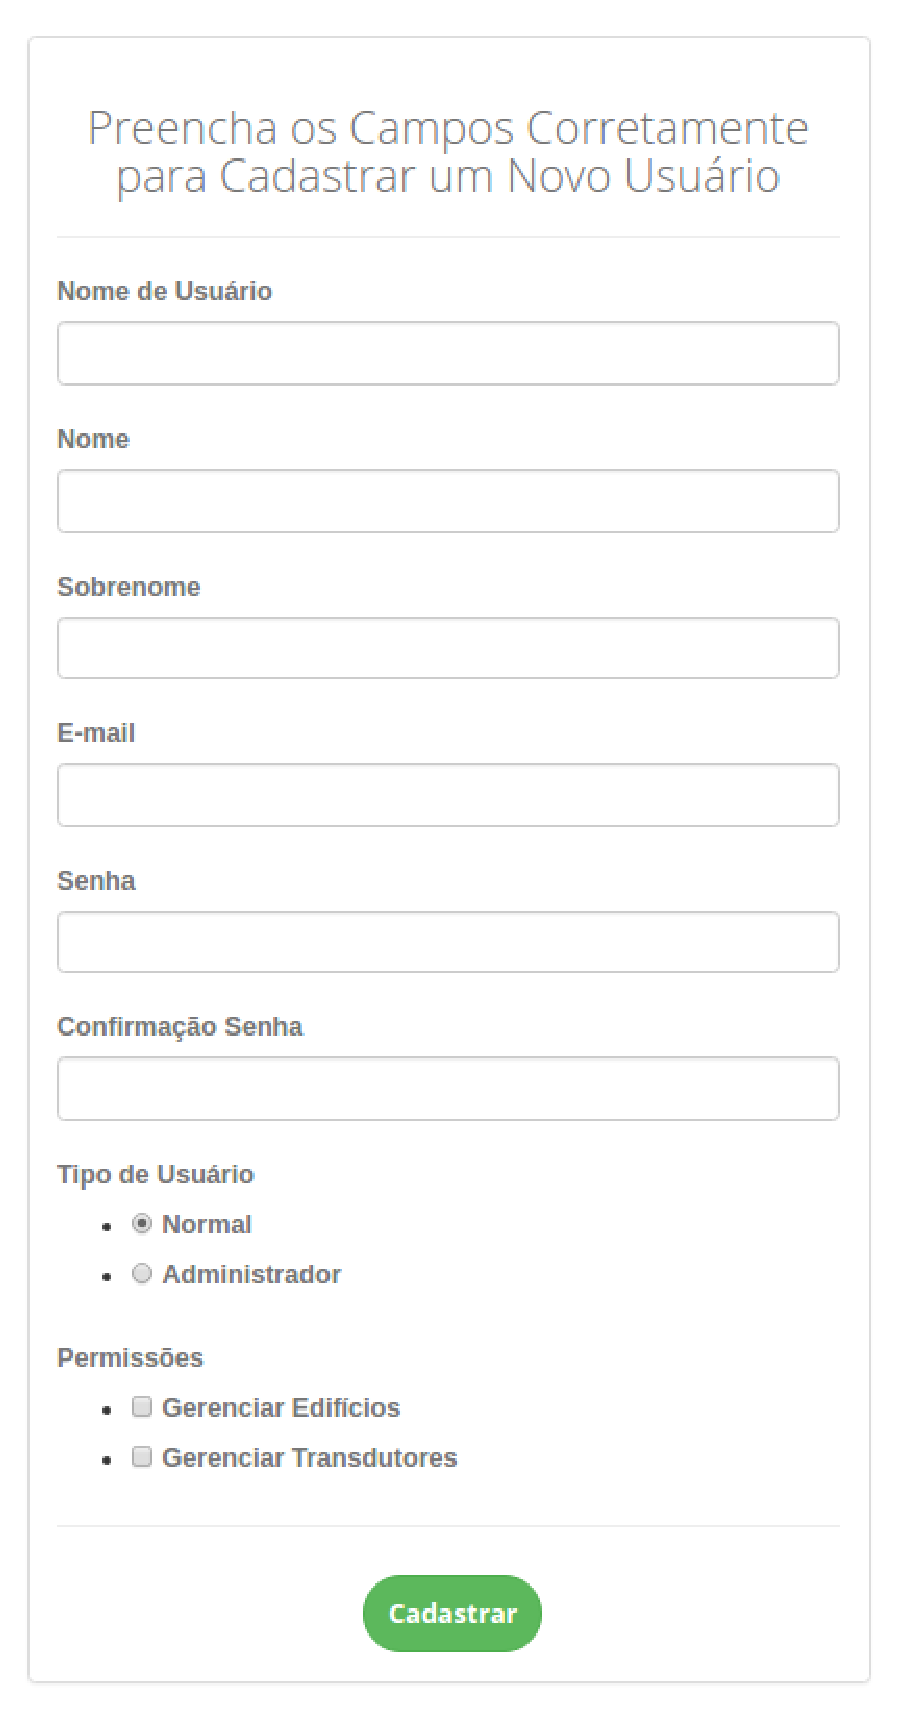
\includegraphics[keepaspectratio=true,scale=0.8]{figuras/img3.eps}
    \caption{Formulário para cadastro de um usuário.}
    \label{img3}
\end{figure}

\begin{figure}[!htpb]
    \centering
    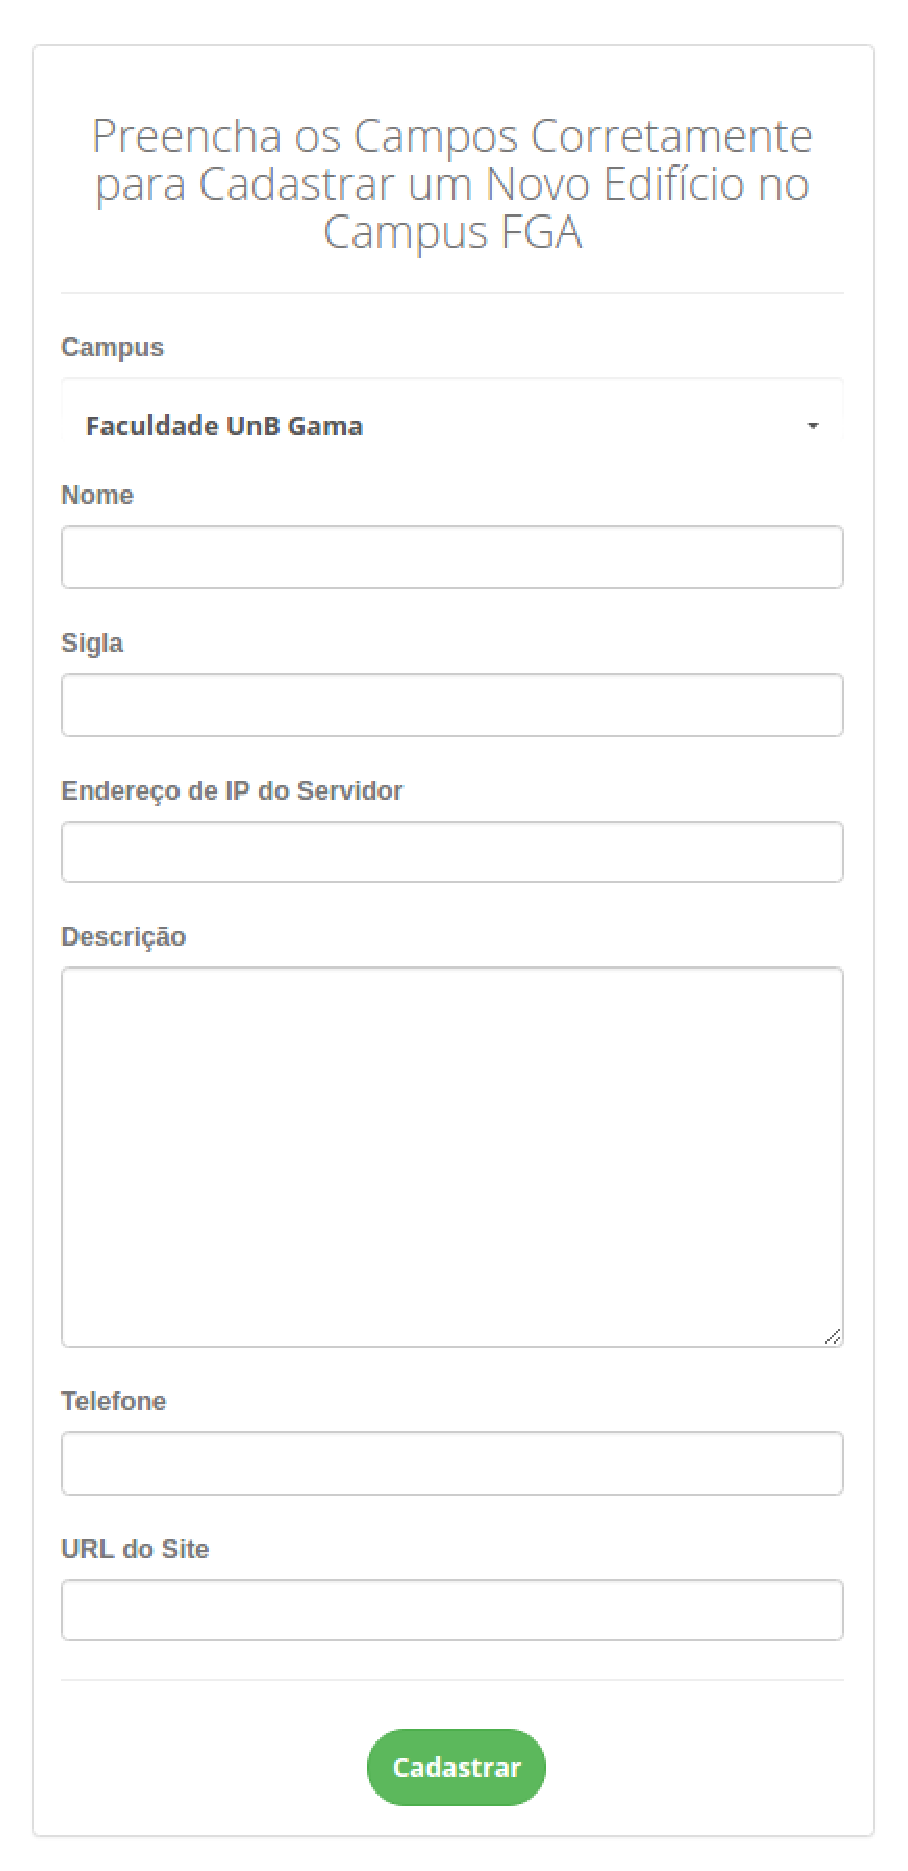
\includegraphics[keepaspectratio=true,scale=0.65]{figuras/img10.eps}
    \caption{Formulário para cadastro de um edifício.}
    \label{img10}
\end{figure}

\begin{figure}[!htpb]
    \centering
    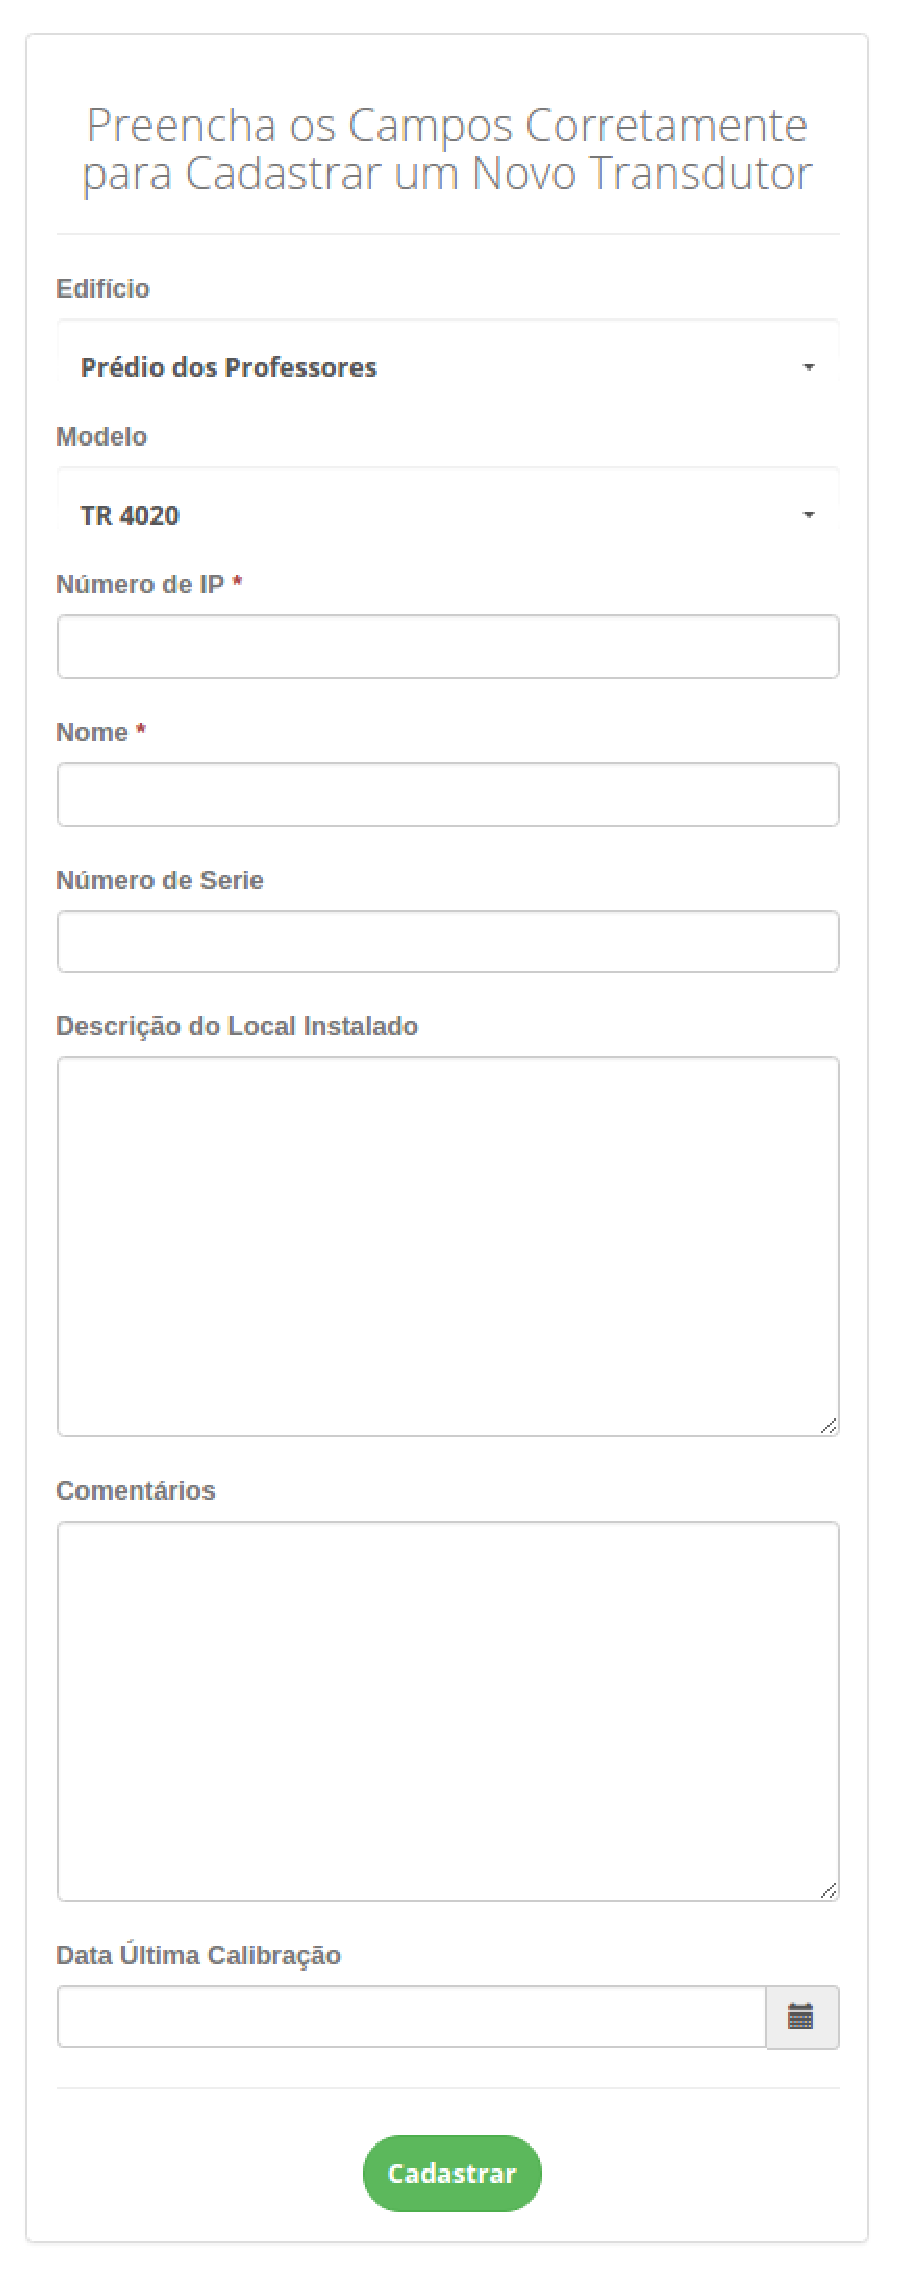
\includegraphics[keepaspectratio=true,scale=0.65]{figuras/img14.eps}
    \caption{Formulário para cadastro de um transdutor.}
    \label{img14}
\end{figure}

\end{apendicesenv}

\begin{anexosenv}

\partanexos

\chapter{Primeiro Anexo}
\begin{figure}[!h]
    \centering
    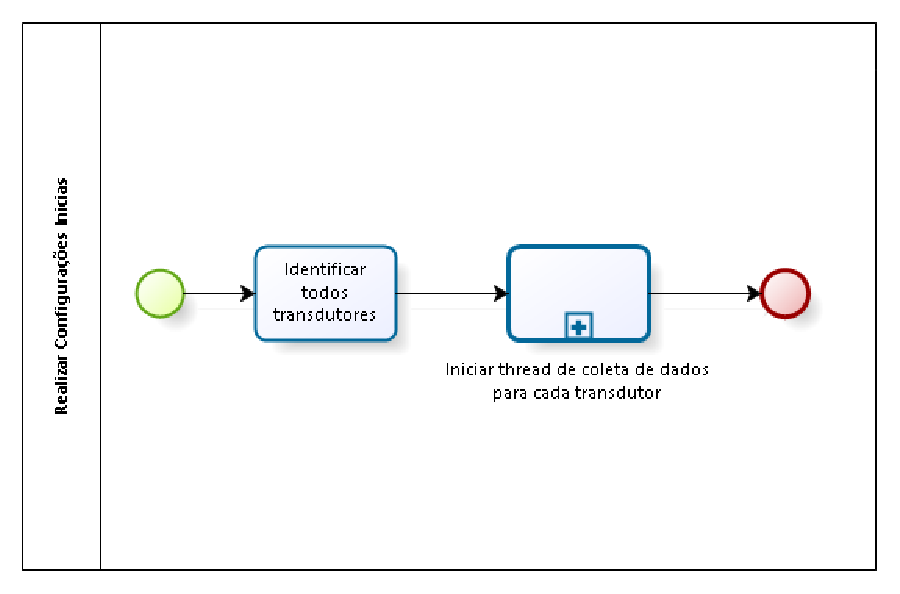
\includegraphics[keepaspectratio=true,scale=1.0]{figuras/process_2.eps}
    \caption{}
    \label{process_2}
\end{figure}

\begin{figure}[!h]
    \centering
    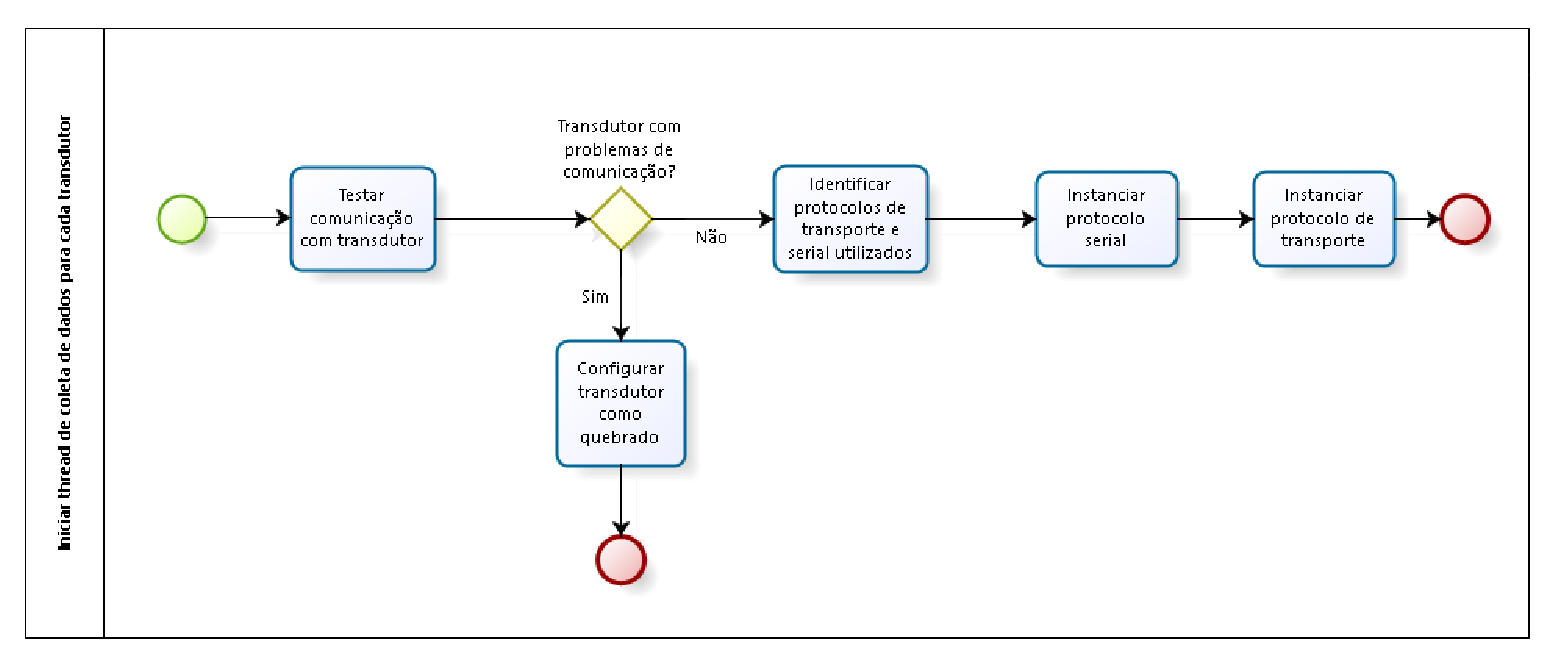
\includegraphics[keepaspectratio=true,scale=0.7,angle=90]{figuras/process_3.eps}
    \caption{}
    \label{process_3}
\end{figure}

\begin{figure}[!h]
    \centering
    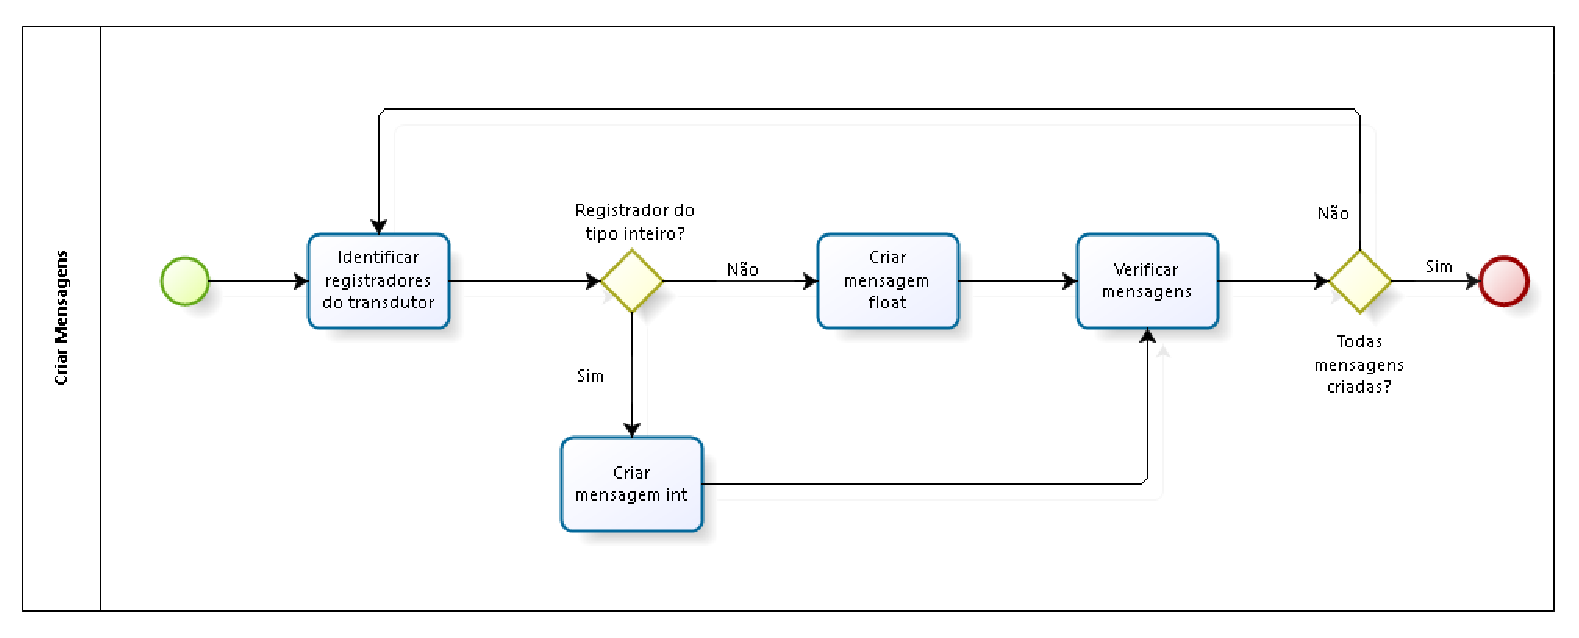
\includegraphics[keepaspectratio=true,scale=0.7,angle=90]{figuras/process_4.eps}
    \caption{}
    \label{process_4}
\end{figure}

\begin{figure}[!h]
    \centering
    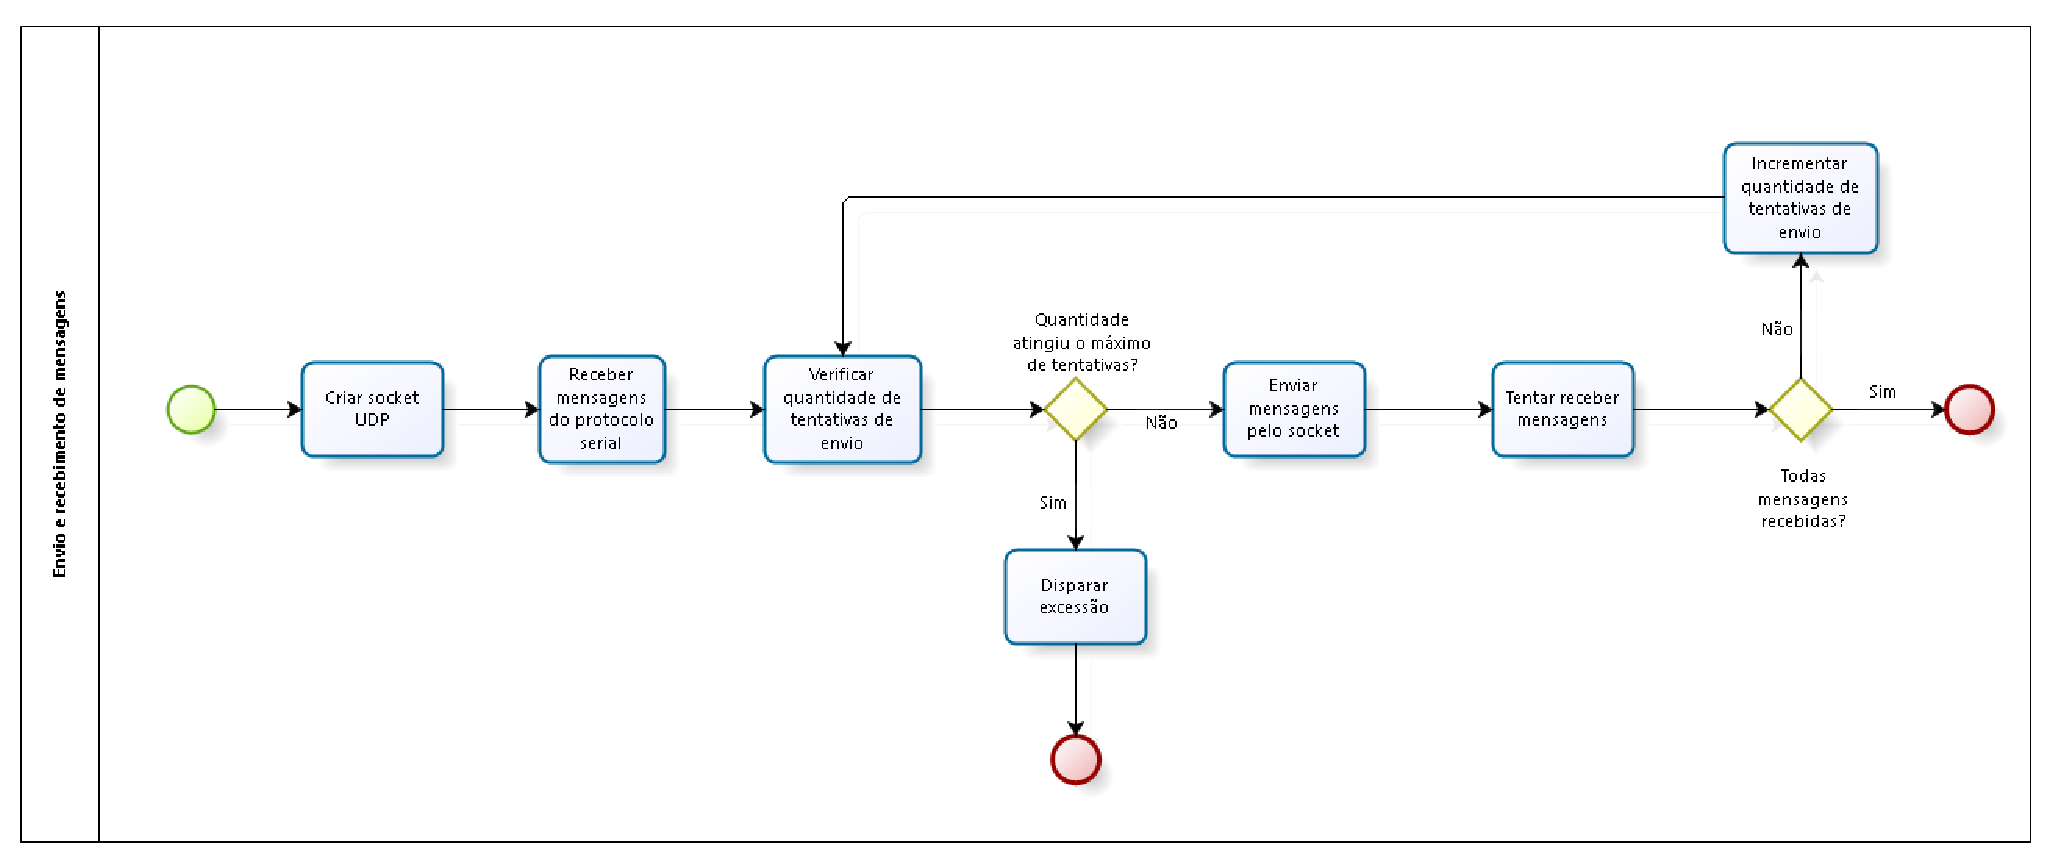
\includegraphics[keepaspectratio=true,scale=0.7,angle=90]{figuras/process_5.eps}
    \caption{}
    \label{process_5}
\end{figure}

\begin{figure}[!h]
    \centering
    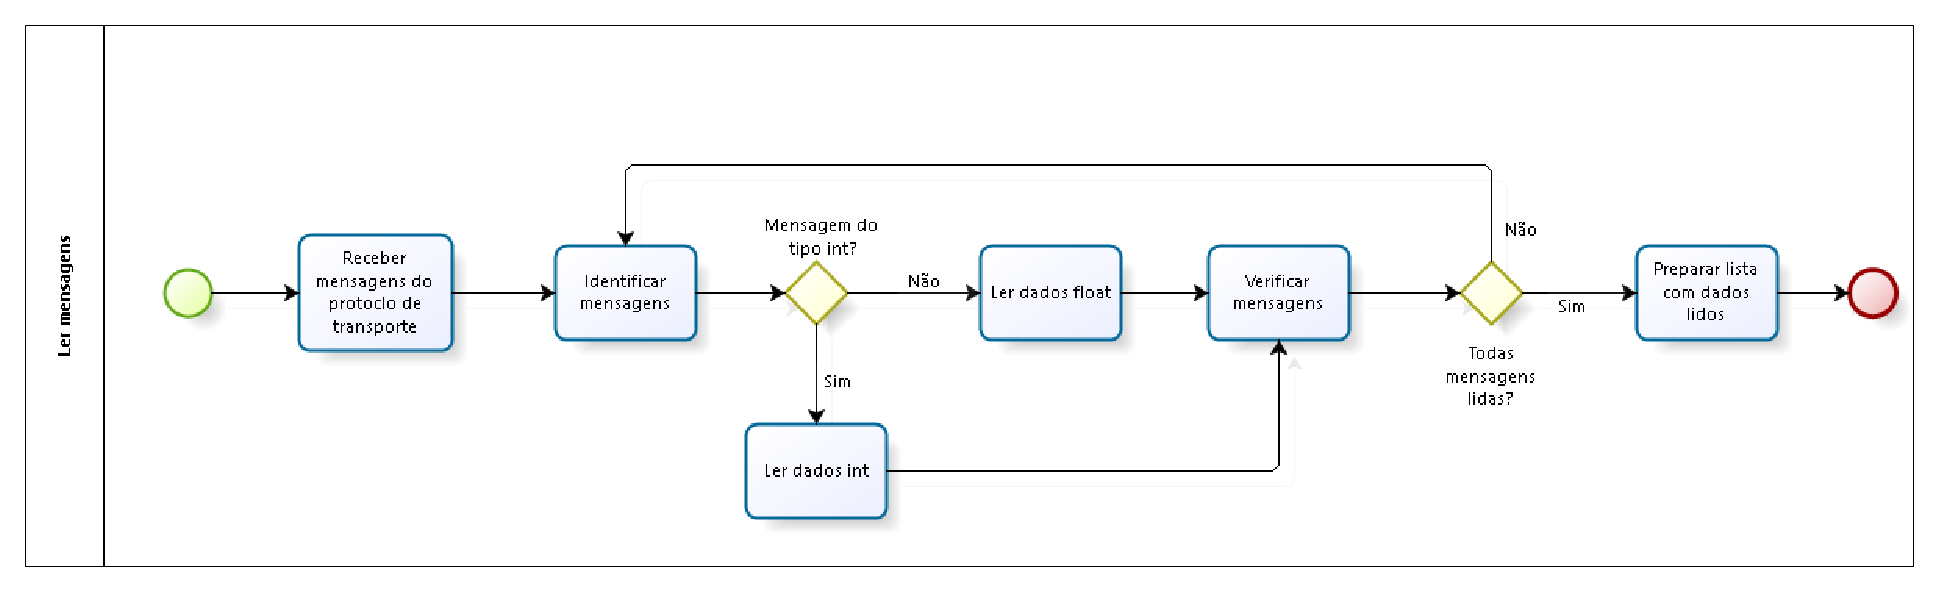
\includegraphics[keepaspectratio=true,scale=0.7,angle=90]{figuras/process_6.eps}
    \caption{}
    \label{process_6}
\end{figure}

\begin{figure}[!h]
    \centering
    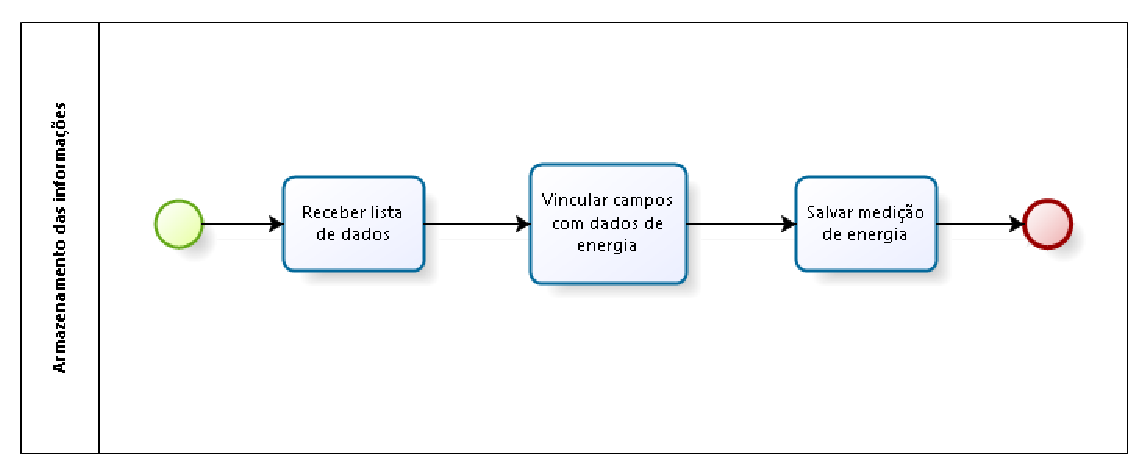
\includegraphics[keepaspectratio=true,scale=1.0]{figuras/process_7.eps}
    \caption{}
    \label{process_7}
\end{figure}

\chapter{Segundo Anexo}

Texto do segundo anexo.

\end{anexosenv}


\printindex

\end{document}

